\documentclass{fkbook}



% For resolution of that one triangulation
\usetikzlibrary{intersections}

% For the tetrahedron thing
\usetikzlibrary{backgrounds}

% For 3d plots
\usepackage{tikz-3dplot}

\usetikzlibrary{external}
\tikzexternalize
\tikzsetexternalprefix{figures/}

\usepackage{fkthm}
% For music note in subtitle

\usepackage{wasysym}

\begin{document}
\pagestyle{plain}
\frontmatter

\fkauthor{Forest Kobayashi}
\fktitle{Homology Theory}
\fksubtitle{Notes \& Exercises from my Independent Study}
\fkalttitle{(Or: \itshape If I could save Klein in a bottle \eighthnote)}
\fkaffiliation{{Department of Mathematics\\}{\itshape Harvey Mudd College\\}}
\fksupervisor{Francis Su}
\fksupervisoraffiliation{Department of Mathematics, Harvey Mudd College}

\maketitlepage
\tableofcontents

\chapter{Introduction}
\section*{What's this?}\noindent\indent
This document is a compendium of notes, exercises, and other miscellany from my
independent study in Homology Theory. For this, I am working through the second
half of \emph{Topology Through Inquiry} by Michael Starbird and Francis Su
(i.e., chapters 11-20), under supervision from Prof.\ Su himself. Rough topic
coverage should be discernable from the table of contents, as I've tried to
name each section identically to the corresponding title in the book.

\section*{Notation}
Most notation I use is fairly standard. Here's a (by no means exhaustive) list
of some stuff I do.
\begin{itemize}
  \item ``WTS'' stands for ``want to show,'' $\st$ for ``such that.'' WLOG, as
    usual, is without loss of generality.
  \item End-of-proof things: $\blacksquare$ is QED for exercises and theorems.
    $\square$ is used in recursive proofs (e.g., proving a Lemma within a
    theorem proof). If doing a proof with casework, $\cmark$ will be used to
    denote the end of each case.
  \item $\contra$ means contradiction
  \item $\mathscr{T}(U)$ will denote the topology of a topological space $U$.
  \item $\mc P(A)$ is the powerset of $A$. I don't like using $2^A$.
  \item $\onto$ denotes surjection.
  \item $\into$ denotes injection.
  \item Thus, $\bij$ denotes bijection.
  \item \textbf{Important:} I use $f\fim[A]$ for the image of $A$ under $f$, and
    $f\fpre[B]$ for the inverse image of $B$ under $f$.
  \item $\sim$ and $\equiv$ are used for equivalence relations. $\cong$ is used
    to denote homeomorphism and isomorphism of groups. $\simeq$ is for Homotopy
    equivalence.
  \item $\epsilon$ is for trivial elements (e.g., the trivial path), while
    $\varepsilon$ is for small positive quantities.
  \item $\ol{U}$ denotes the closure of $U$, $\interior{U}$ is the interior of
    $U$.
  \item $A^c$ is $A$ complement.
  \item $\simp{k}$ denotes a simplex on $k+1$ vertices (that is, a $k$-simplex).
    $\simpdel{i}{k}$ is the same simplex with the $i$\textsuperscript{th} vertex
    deleted.
  \item $[n] = \set{i \MID i = 0,1,\ldots, n}$.
\end{itemize}

\mainmatter

\pagestyle{main}

\chapter[Homological Prereqs]{Manifolds, Simplexes Complexes, and Triangulability: Building Blocks}

\section{Manifolds}
We define some basic Euclidean sets for use in homeomorphisms.
\begin{definition}[$n$-cube]
  The \emph{$n$-dimensional cube}, denoted $\DD^n$, is defined as
  \begin{align*}
    \DD^n
    &= \set{\pn{x_1, \ldots, x_n} \in \RR^n \MID 0 \leq x_i \leq 1 \text{ for } i = 1, \ldots, n} \\
    &= \overbrace{[0,1] \times [0,1] \times \cdots \times [0,1]}_{n \text{ times}} \subset \RR^n.
  \end{align*}
\end{definition}
\begin{definition}[$n$-ball]
  The \emph{standard $n$-ball}, denoted $B^n$, is
  \[
    B^n = \set{\pn{x_1, \ldots, x_n} \in \RR^n \MID x_1^2 + \cdots + x^2_n \leq
      1}.
  \]
\end{definition}
\begin{definition}[$n$-sphere]
  The \emph{standard $n$-sphere}, denoted $\sS^n$, is
  \[
    \sS^n = \set{(x_0, \ldots, x_n) \in \RR^{n+1} \MID x^2_0 + \cdots + x^2_n =
      1}.
  \]
  note that here, our indices start at $0$.
\end{definition}
\begin{definition}[$n$-manifold]
  An \emph{$n$-dimensional manifold} or \emph{$n$-manifold} is a separable
  metric space $M$ such that $\forall p \in M$, $\exists U \in \ms T(M) \st p
  \in U$ and $U \cong V \subset \RR^n$.
\end{definition}
\begin{problem}[15.8]
  If $M$ is an $n$-manifold and $U$ is an open subset of $M$, then $U$ is also
  an $n$-manifold.
\end{problem}
\begin{problem}[15.9]
  If $M$ is an $m$-manifold and $N$ is an $n$-manifold, then $M \times N$ is an
  $(m+n)$-manifold.
\end{problem}
\begin{problem}[15.10]
  Let $M^n$ be an $n$-dimensional manifold with boundary. Then $\partial M^n$ is
  an $(n-1)$-manifold.
\end{problem}
\section{Simplicial Complexes}~
\begin{definition}[Affine Independence]
  Let $X = \set{v_0, \ldots, v_k} \subset \RR^n$. We say $X$ is \emph{affinely
    independent} if $\set{v_1 - v_i, \ldots, v_k - v_i}$ is linearly
  independent for all $v_i$.
\end{definition}
\begin{example}
  $X = \set{(0,1), (-\sqrt{3}/2, -1/2), (\sqrt{3}/2, -1/2)}$ is affinely
  independent.
\end{example}
\begin{definition}[Convex combination]
  A \emph{convex combination} of $v_0, \ldots, v_k$ is a linear combination
  of these points whose coefficients are nonnegative and sum to 1.
\end{definition}
\begin{definition}[$k$-simplex]
  A \emph{$k$-simplex} is the set of all convex combinations of $k+1$ affinely
  independent points in $\RR^n$. For affinely independent points $v_0, \ldots,
  v_k$ in $\RR^n$, $\set{v_0\cdots v_k}$ denotes the $k$-simplex
  \[
    \set{\lambda_0 v_0 + \lambda_1v_1 + \cdots + \lambda_kv_k \MID \forall i =0,
      1, \ldots, k;\ 0 \leq \lambda_i \leq 1 \text{ and } \sum_{i=0}^k \lambda_i
    = 1}
  \]
  each $v_i$ is called a \emph{vertex} of $\set{v_0 \cdots v_k}$. Any point $x$
  in the $k$-simplex is specified uniquely by the $k+1$ coefficients
  $(\lambda_i)$; these coefficients are called the \emph{barycentric coordinates
    of $x$.} The \emph{barycentric coordinate of $x$ with respect to vertex
    $v_i$} is the coefficient $\lambda_i$.
\end{definition}
\begin{definition}[Face and dimension]
  Any simplex $\tau$ whose vertices are a nonempty subset of the vertices of a
  $k$-simplex $\sigma$ is called a \emph{face} of $\sigma$. If the number of
  vertices is $i+1$, then $\tau$ has \emph{dimension} $i$ and is called an
  $i$-face of $\sigma$ and $\tau$ has \emph{codimension} $k-i$, the number of
  dimensions below the top dimension.
\end{definition}
\textbf{Notational Note:} if $\sigma = \simp k$, the $(k-1)$-dimensional face of
$\sigma$ obtained by deleting the vertex $v_j$ from the list of vertices of
$\sigma$ is denoted by $\simpdel{i}{k}$.
\begin{problem}[15.11]
  Show that if $\sigma$ is a simplex and $\tau$ is one of its faces, then $\tau
  \subset \sigma$.
\end{problem}
\begin{solution}
  This is fairly trivial, so we offer just a sketch. Suppose $\mb v \in \tau$.
  Then write $\mb v$ as an element of $\sigma$ by taking $\lambda_i = 0$ for all
  those $v_i \not \in \tau$.
\end{solution}
\begin{definition}[Simplicial complex]
  A \emph{simplicial complex} $K$ (in $\RR^n$) is a collection of simplicies in
  $\RR^n$ satisfying the following conditions.
  \begin{enumerate}[label=\arabic*.]
    \item If a simplex $\sigma$ is in $K$, then each face of $\sigma$ is also in
      $K$.
    \item Any two simplices in $K$ are either disjoint or their intersection is
      a face of each.
  \end{enumerate}
\end{definition}
\begin{problem}[15.13]
  Exhibit a collection of simplices that satisfies condition (1) but not
  condition (2) in the definition of a simplicial complex.
\end{problem}
\begin{solution}
  Consider the following diagram, where the interior of each simplex is taken to
  be in the complex.
  \begin{figure}[H]
    \centering
    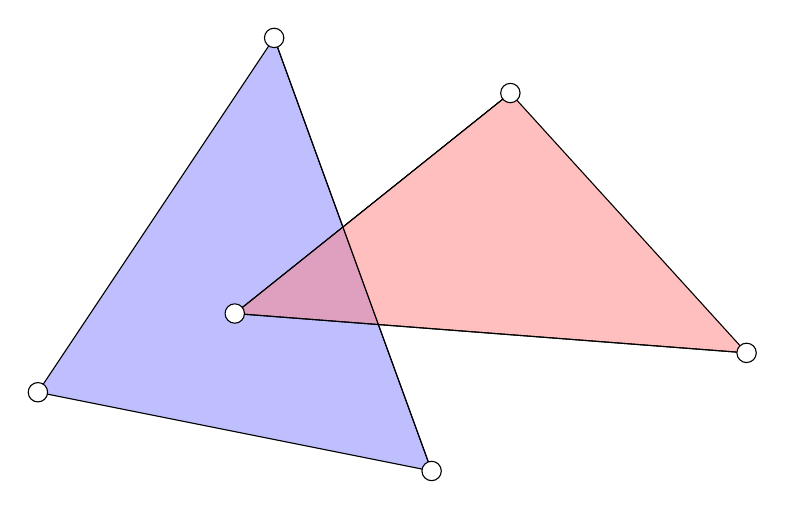
\begin{tikzpicture}[every node/.style={circle,draw=black, fill=white, inner sep=0pt,minimum size=7pt}]
      % Simplex 1
      \coordinate (A) at (0,0);
      \coordinate (B) at (3,4.5);
      \coordinate (C) at (5,-1);

      % Simplex 2
      \coordinate (D) at (2.5,1);
      \coordinate (E) at (6,3.8);
      \coordinate (F) at (9,.5);

      \draw[fill=blue!50!white, fill opacity=.5] (A) -- (B) -- (C) -- (A);
      \draw[fill=red!50!white, fill opacity=.5] (D) -- (E) -- (F) -- (D);

      \draw[name path=B--C] (B) -- (C);
      \draw[name path=D--E] (D) -- (E);
      \draw[name path=D--F] (D) -- (F);

      \path[name intersections={of=B--C and D--E, by=G}];
      \path[name intersections={of=B--C and D--F, by=H}];

      % nodes for simplex (1)
      \node (a) at (A) {};
      \node (b) at (B) {};
      \node (c) at (C) {};

      % nodes for simplex (2)
      \node (d) at (D) {};
      \node (e) at (E) {};
      \node (f) at (F) {};
    \end{tikzpicture}
    \caption{An unfortunate collision}
    \label{fig:non-simplicial-complex}
  \end{figure}
  Note that to fix this sorry situation, we can't just add two vertices at the
  points of intersections of the lines above (then the intersection of the
  resulting simplex with the two shone above would be non-trivial, but still not
  a face of the larger ones). We'd actually need something much more
  complicated.
  \begin{figure}[H]
    \centering
    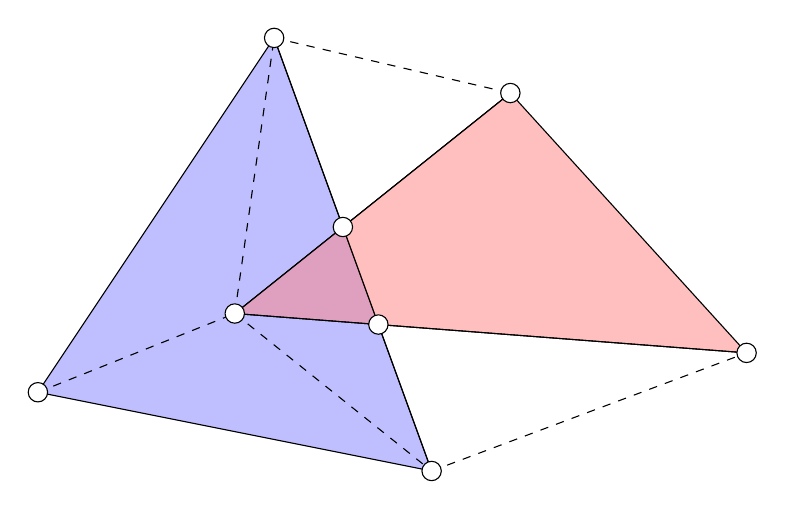
\begin{tikzpicture}[every node/.style={circle,draw=black, fill=white, inner sep=0pt,minimum size=7pt}]
      % Simplex 1
      \coordinate (A) at (0,0);
      \coordinate (B) at (3,4.5);
      \coordinate (C) at (5,-1);

      % Simplex 2
      \coordinate (D) at (2.5,1);
      \coordinate (E) at (6,3.8);
      \coordinate (F) at (9,.5);

      \draw[fill=blue!50!white, fill opacity=.5] (A) -- (B) -- (C) -- (A);
      \draw[fill=red!50!white, fill opacity=.5] (D) -- (E) -- (F) -- (D);

      \draw[name path=B--C] (B) -- (C);
      \draw[name path=D--E] (D) -- (E);
      \draw[name path=D--F] (D) -- (F);

      \path[name intersections={of=B--C and D--E, by=G}];
      \path[name intersections={of=B--C and D--F, by=H}];

      \draw[dashed] (B) -- (E);
      \draw[dashed] (C) -- (F);
      \draw[dashed] (A) -- (D);
      \draw[dashed] (D) -- (B);
      \draw[dashed] (D) -- (C);

      \node (g) at (G) {};
      \node (h) at (H) {};

      % nodes for simplex (1)
      \node (a) at (A) {};
      \node (b) at (B) {};
      \node (c) at (C) {};

      % nodes for simplex (2)
      \node (d) at (D) {};
      \node (e) at (E) {};
      \node (f) at (F) {};
    \end{tikzpicture}
    \caption{Constructing a resolution}
    \label{fig:constructing-a-resolution}
  \end{figure}
  \begin{figure}[H]
    \centering
    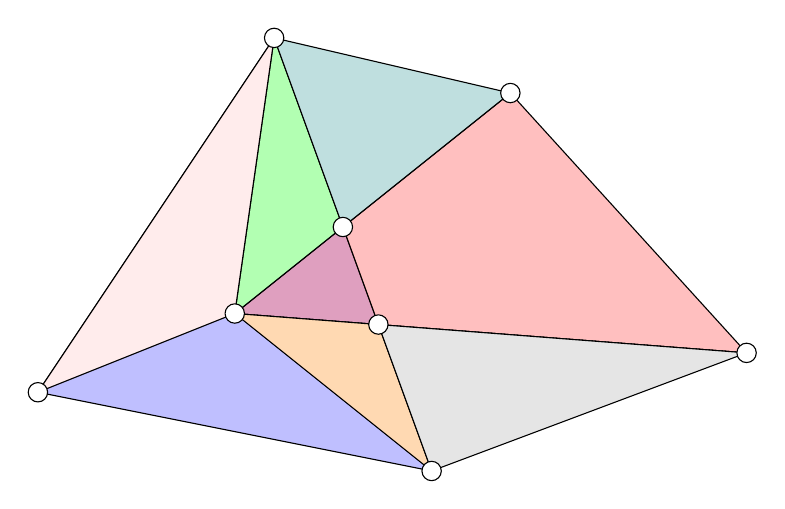
\begin{tikzpicture}[every node/.style={circle,draw=black, fill=white, inner sep=0pt,minimum size=7pt}]
      % Simplex 1
      \coordinate (A) at (0,0);
      \coordinate (B) at (3,4.5);
      \coordinate (C) at (5,-1);

      % Simplex 2
      \coordinate (D) at (2.5,1);
      \coordinate (E) at (6,3.8);
      \coordinate (F) at (9,.5);

      \draw[fill=blue!50!white, fill opacity=.5] (A) -- (B) -- (C) -- (A);
      \draw[fill=red!50!white, fill opacity=.5] (D) -- (E) -- (F) -- (D);

      \draw[name path=B--C] (B) -- (C);
      \draw[name path=D--E] (D) -- (E);
      \draw[name path=D--F] (D) -- (F);

      \path[name intersections={of=B--C and D--E, by=G}];
      \path[name intersections={of=B--C and D--F, by=H}];

      \draw[fill=green!30!white] (B) -- (G) -- (D) -- (B);
      \draw[fill=orange!30!white] (H) -- (C) -- (D) -- (H);
      \draw[fill=pink!30!white] (A) -- (B) -- (D) -- (A);
      \draw[fill=teal!25!white] (B) -- (E) -- (G) -- (B);
      \draw[fill=black!10!white] (H) -- (F) -- (C) -- (H);

      \node (g) at (G) {};
      \node (h) at (H) {};

      % nodes for simplex (1)
      \node (a) at (A) {};
      \node (b) at (B) {};
      \node (c) at (C) {};

      % nodes for simplex (2)
      \node (d) at (D) {};
      \node (e) at (E) {};
      \node (f) at (F) {};
    \end{tikzpicture}
    \caption{The completed resolution}
    \label{fig:completed-resolution}
  \end{figure}
\end{solution}
\begin{definition}[Underlying space]
  The \emph{underlying space} $\abs{K}$ of a simplicial complex $K$ is the set
  \[
    \abs{K} = \bigcup_{\sigma \in K} \sigma,
  \]
  the union of all simplices in $K$, with a topology consisting of sets whose
  intersection with each simplex $\sigma \in K$ is open in $\sigma$. For finite
  simplicial complexes, this topology is the topology inherited as a subspace of
  $\RR^n$.
\end{definition}
\begin{problem}[15.14]
  Let $K$ be the following simplicial complex:
  \[
    \text{(Omitted because it takes a long time to TeX out)}
  \]
  draw $K$ and its underlying space.
\end{problem}
\begin{solution}
  \begin{figure}[H]
    \centering
    \begin{minipage}{.49\linewidth}
      \centering
      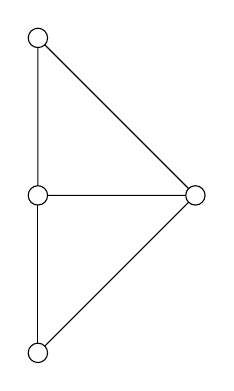
\begin{tikzpicture}[scale=2, every node/.style={circle,draw=black, fill=white, inner sep=0pt,minimum size=7pt}]

        \coordinate (A) at (0,0);
        \coordinate (B) at (0,1);
        \coordinate (C) at (1,0);
        \coordinate (D) at (0,-1);

        \draw (A) -- (B) -- (C) -- (A);
        \draw (A) -- (D);
        \draw (D) -- (C);

        \node (a) at (A) {};
        \node (b) at (B) {};
        \node (c) at (C) {};
        \node (d) at (D) {};

      \end{tikzpicture}
    \end{minipage}
    \begin{minipage}{.49\linewidth}
      \centering
      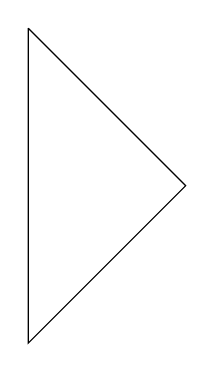
\begin{tikzpicture}[scale=2, every node/.style={circle,draw=black, fill=white, inner sep=0pt,minimum size=7pt}]

        \coordinate (B) at (0,1);
        \coordinate (C) at (1,0);
        \coordinate (D) at (0,-1);

        \draw (B) -- (C) -- (D) -- (B);
      \end{tikzpicture}
    \end{minipage}
    \caption{$K$ (left) and its underlying space (right).}
  \end{figure}
\end{solution}
\begin{definition}[Triangulable]
  A topological space $X$ is said to be \emph{triangulable} if it is
  homeomorphic to the underlying space of a simplicial complex $K$. In that
  case, we say $K$ is a \emph{triangulation} of $X$.
\end{definition}
\begin{problem}[15.15]
  Show that the space shown in Figure 15.2 (not included here) is triangulable
  by exhibiting a simplicial complex whose underlying space it is homeomorphic
  to.
\end{problem}
\begin{solution}
  \begin{figure}[H]
    \centering
    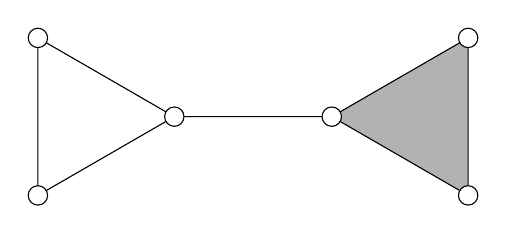
\begin{tikzpicture}[scale=2, every node/.style={circle,draw=black, fill=white, inner sep=0pt,minimum size=7pt}]

      \coordinate (A) at (0,0);
      \coordinate (B) at (-.866,.5);
      \coordinate (C) at (-.866,-.5);
      \coordinate (D) at (1,0);
      \coordinate (E) at (1.866,.5);
      \coordinate (F) at (1.866,-.5);

      \draw (A) -- (B) -- (C) -- (A) -- (D);
      \draw[fill=black!30!white] (D) -- (E) -- (F) -- (D);

      \node (a) at (A) {};
      \node (b) at (B) {};
      \node (c) at (C) {};
      \node (d) at (D) {};
      \node (e) at (E) {};
      \node (f) at (F) {};

    \end{tikzpicture}
    \caption{Such a simplicial complex. Note, the left triangle is unfilled.}
  \end{figure}
\end{solution}
\begin{problem}[15.6]
  For each $n \in \NN$, $\sS^n$ is triangulable.
\end{problem}
\begin{proof}
  We proceed by induction.

  \begin{induction}
    \item Note that $S^0$ is trivially triangulable by taking $K =
      \set{\set{v_0}, \set{v_2}}$.
    \item Suppose that for $k \in \NN \cup \set{0}$, $\sS^k$ is triangulable by
      a simplicial complex $K$.
    \item Take $v_{k+1} \in \RR^{k+1}$ such that $v_{k+1} \in
      (\vspan{K})^\perp$. Then
  \end{induction}
  {\color{red} This proof is unfinished. Hey, future Forest --- you should
    return to this later!}
\end{proof}
\section{Simplicial Maps and PL Homeomorphisms}
We now define structure-preserving maps bewteen simplicial concepts.
\begin{definition}[Simplicial map]
  Let $X,Y$ be topological spaces. A function $f : X \to Y$ is called a
  \emph{simplicial map} iff there exist simplicial complexes $K$ and $L$ such
  that $\abs{K} = X$, $\abs{L} = Y$, and $f$ maps each simplex of $K$ linearly
  onto a (possibly lower-dimensional) simplex in $L$.
\end{definition}
\begin{definition}[Simplicially homeomorphic]
  A simplicial map $f$ is a simplicial homomorphism iff it's a bijection; in
  that case, the two complexes are \emph{simplicially homeomorphic}
\end{definition}
\begin{problem}[15.17]
  A simplicial map from $K$ to $L$ is determined by the images of the vertices
  of $K$.
\end{problem}
\begin{solution}
  Apply linearity and show the analog of images of liner combinations being
  uniquely determined by the action on the basis.
\end{solution}
\begin{problem}[15.18]
  A composition of simplicial maps is a simplicial map.
\end{problem}
\begin{solution}
  Simply plug in arbitrary points and verify the properties hold.
\end{solution}
\begin{definition}[Subdivision]
  Let $K$ be a simplicial complex. Then a simplicial complex $K'$ is a
  \emph{subdivision} of $K$ iff each simplex of $K'$ is a subset of a simplex of
  $K$ and each simplex of $K$ is the union of finitely many simplices of $K'$.
\end{definition}
\begin{definition}[Piecewise linear]
  If $K$ and $L$ are complexes, a continuous map $f : \abs{K} \to \abs{L}$ is
  called \emph{piecewise linear} or \emph{PL} if and only if there are
  subdivisions $K'$ of $K$ and $L'$ of $L$ such that $f$ is a simplicial map
  from $K'$ to $L'$. If there exist subdivisions such that $f$ is a simplicial
  homomorphism, then $f$ is a \emph{PL homeomorphism} and the spaces are
  \emph{PL homeomorphic.}
\end{definition}
\begin{problem}[15.21]
  A composition of PL maps is PL. A PL homeomorphism is an equivalence relation.
\end{problem}
\begin{solution}
  Let $K,L,M$ be complexes, and let $g : \abs{K} \to \abs{L}$, $f : \abs{L} \to
  \abs{M}$ be continuous PL maps. WTS $h = f \circ g$ is a PL map.

  Let $K', L', M'$ be the corresponding subdivisions of $K,L,$ and $M$,
  respectively. Then $g$ is a simplicial map from $K'$ to $L'$, and $f$ is a
  simplicial map from $L'$ to $M'$. Then $\forall \sigma \in K'$, $g(\sigma) \in
  L'$, whence $f(g(\sigma)) \in M'$. It follows that $h = g \circ f$ is a
  simplicial map from $K'$ to $M'$.

  We give a sketch of the proof that PL homeomorphism is an equivalence
  relation. To verify reflexivity, take the identity map. Symmetry follows by
  inverting the simplicial homeomorphism. Transitivity follows by the above.
  Thus, the claim holds.
\end{solution}
% \begin{problem}[15.22]
%   PL homeomorphic complexes are homeomorphic as topological spaces.
% \end{problem}
% \begin{solution}
% \end{solution}
\section{Simplicial Approximation}
\begin{problem}[15.23]
  Let $K$ be a complex consisting of the boundary of a triangle (three vertices
  and three edges) and $L$ be an isomorphic complex. Both $\abs{K}$ and
  $\abs{L}$ are topologically circles. There is a continuous map that takes the
  circle $\abs{K}$ and winds it twice around the circle $\abs{L}$; however, show
  that there is no simplicial map from $K$ to $L$ that winds the circle
  $\abs{K}$ twice around the circle $\abs{L}$.
\end{problem}
\begin{solution}
  We offer a brief sketch. Basically, this would require each 1-simplex to map
  to two 1-simplices. Contradiction.
\end{solution}
\begin{definition}[Barycenter]
  The \emph{barycenter} of a $k$-simplex $\simp{k}$ in $\RR^n$ is the point
  $\frac{1}{k+1} \pn{v_0 + \cdots + v_k}$.
\end{definition}
\begin{definition}[First barycentric subdivision ($\sd \sigma$)]
  Let $\sigma$ be an $n$-simplex. The \emph{first barycentric subdivision of
    $\sigma$}, denoted $\sd \sigma$, is the complex of all simplices of the form
  $\simp[b]{k}$, where $b_i$ is the barycenter of a face $\sigma^i$ of $\sigma$
  from a chain of faces of $\sigma$,
  \[
    \sigma^0 \subset \sigma^1 \subset \cdots \subset \sigma^k
  \]
  of increasing (not necessarily consecutive) dimensions. The maximal simplices,
  that is, the $n$-simplices of $\sd \sigma$ each arise from a maximal sequence
  of faces, that is, from faces of consecutive dimensions starting with a vertex
  of $\sigma$. Thus an $n$-simplex of $\sd \sigma$ corresponds exactly to a
  permutation of the vertices of $\sigma$.
\end{definition}
\begin{definition}[$\sd K$]
  Let $K$ be a simplicial complex. The \emph{first barycentric subdivision} of
  $K$, denoted $\sd K$, is the complex consisting of all the simplices in the
  barycentric subdivision of each simplex of $K$.
\end{definition}
\begin{definition}[$m$-th barycentric subdivision]
  The \emph{second barycentric subdivision}, denoted $\sd^2 K$, is the first
  barycentric subdivision of $\sd K$. Proceeding in this way, the \emph{$m$-th
    barycentric subdivision} is denoted $\sd^m K$.
\end{definition}
Some diagrams:
\begin{figure}[H]
  \centering
  \begin{subfigure}{.45\linewidth}
    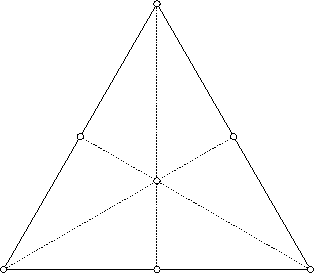
\includegraphics[width=\linewidth]{figures/barycentric-1.pdf}
  \end{subfigure}
  \hspace{1cm}
  \begin{subfigure}{.45\linewidth}
    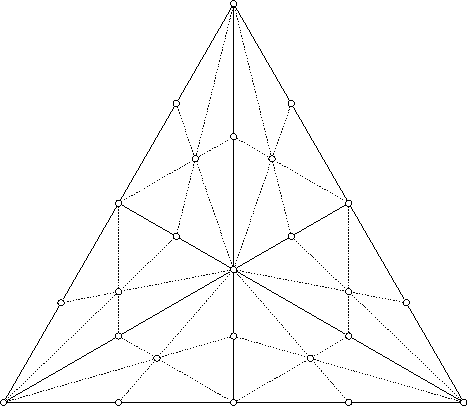
\includegraphics[width=\linewidth]{figures/barycentric-2.pdf}
  \end{subfigure}\\[2cm]
  \begin{subfigure}{.45\linewidth}
    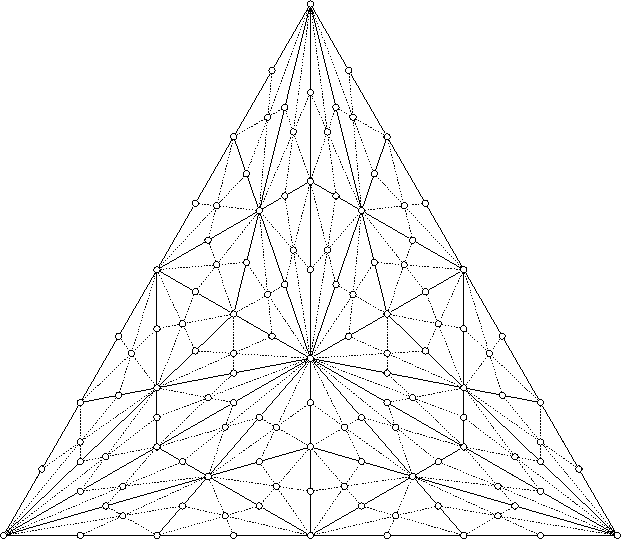
\includegraphics[width=\linewidth]{figures/barycentric-3.pdf}
  \end{subfigure}
  \hspace{1cm}
  \begin{subfigure}{.45\linewidth}
    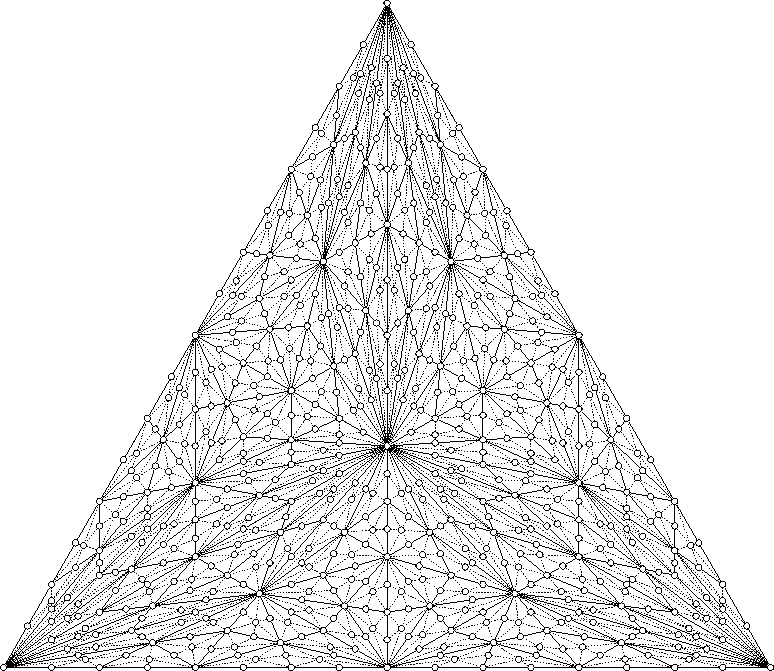
\includegraphics[width=\linewidth]{figures/barycentric-4.pdf}
  \end{subfigure}
  \caption{The first 4 barycentric subdivisions}
  \label{fig:subdivs}
\end{figure}
\begin{problem}[15.24]
  How many $n$-simplices are there in the first barycentric subdivision of an
  $n$-simplex?
\end{problem}
\begin{solution}
  A simple induction shows there are $6^n$ $n$-simplices.
\end{solution}
\begin{problem}[15.25]
  Convince yourself that the barycentric subdivision of a complex $K$ is, in
  fact, a subdivision of $K$.
\end{problem}
\begin{solution}
  I'm convinced.
\end{solution}
\begin{problem}[15.26]
  Let $K$ be a finite simplicial complex and let $a_n$ be the maximum among the
  diameters of simplices in $\sd^n K$. Then
  \[
    \lim_{n\to\infty} a_n = 0.
  \]
\end{problem}
\begin{solution}
  First, we calculate the diameter of an $n$-simplex.
  \begin{leftbar}
    \begin{lemma}
      Let $\sigma_n$ be an $n$-simplex. Then the diameter of $\sigma_n$
      \[
        D = \sup_{\mathclap{\Xx,\, \Yy \in \sigma_n}} \norm{\Xx - \Yy}_2
      \]
      is given by the maximum distance between vertices in the simplex:
      \[
        D = \sup_{\mathclap{\Vv_i, \Vv_j}} \norm{\Vv_i - \Vv_j}_2
      \]
    \end{lemma}

    \emph{Proof of Lemma:} Let $\Xx, \Yy \in \sigma_n$ be arbitrary. It will
    suffice to show that $\Yy$ is not a vertex in $\sigma_n$, then there exists
    a vertex $\Vv \in \sigma_n$ such that $\norm{\Xx - \Yy}_2 < \norm{\Xx -
      \Vv}_2$.

    Write $\Yy$ as convex combinations by
    \begin{align*}
      \Yy &= \sum_{i=0}^n \mu_i \Vv_i.
    \end{align*}
    and observe that since $\sum_{i=0}^n \mu_i = 1$, we have
    \[
      \Xx = \sum_{i=0}^n \mu_i \Xx = \Xx.
    \]
    Then
    \begin{align*}
      \norm{\Xx - \Yy}_2
      &= \norm{\sum_{i=0}^n \Xx - \mu_i\Vv_i}_2 \\
      &= \norm{\sum_{i=0}^n \mu_i(\Xx - \Vv_i)}_2 \\
      &\leq \sum_{i=0}^n \mu_i \norm{\Xx - \Vv_i}_2 \\
      &\leq \sum_{i=0}^n \mu_i \sup_{\Vv_i} \norm{\Xx - \Vv_i}_2 \\
      &= \sup_{\Vv_i} \norm{\Xx - \Vv_i}_2.
    \end{align*}
    Hence, we see for arbitrary $\Yy$, $\norm{\Xx - \Yy}_2 \leq \sup_{\Vv_i}
    \norm{\Xx - \Vv_i}_2$. Now, apply the same result to $\Xx' = \argmax_{\Vv_i}
    \norm{\Xx - \Vv_i}_2$ and $\Yy' = \Xx$ to obtain
    \[
      \norm{\Xx - \Yy}_2 \leq \sup_{\Vv_i} \norm{\Xx - \Vv_i}_2 \leq
      \sup_{\Vv_j}\pn{ \sup_{\Vv_i} \norm{\Vv_j - \Vv_i}} = \sup_{\Vv_i, \Vv_j}
      \norm{\Vv_j - \Vv_i}_2
    \]
    as desired.
  \end{leftbar}
  By the lemma, $a_n$ is given by the maximal side length of a 2-simplex in
  $\sd^n K$. Hence
  \[
    0 \leq a_n \leq \frac{1}{2^n} \frac{2}{\sqrt{3}} \quad \text{\color{red}
      This bound is incorrect. How can I fix it?}
  \]
  and so by the squeeze theorem,
  \[
    \lim_{n\to\infty} a_n = 0
  \]
  as desired.
\end{solution}
\begin{definition}[Minimal face]
  Let $K$ be a simplicial complex. The \emph{minimal face} of $x \in \abs{K}$ is
  the simplex of $K$ of smallest dimension that contains $x$.
\end{definition}
\begin{definition}[Star of vertex]
  The \emph{star of a vertex} $v$ in $K$, denoted $\St(v)$, is the set of all
  points whose minimal face contains $v$.
\end{definition}
\begin{remark}
  The definition of the star of a vertex is basically the interior of the union
  of all simplices containing $v$.
\end{remark}
\begin{problem}[15.27]
  The star of a vertex $v$ in a complex $K$ is an open set of $\abs{K}$, and the
  collection of all vertex stars covers $\abs{K}$.
\end{problem}
\begin{solution}
  Let $v \in K$ be a vertex. Let $x \in \St(v)$ be arbitrary. WTS $\exists
  \varepsilon > 0 \st B_{\epsilon}(x) \subset \St(v)$. We have the following
  cases:
  \begin{enumerate}[label=(\arabic*)]
    \item Suppose $x = v$. Then taking $\epsilon = \frac{1}{2} \inf_{\Vv_i}
      \abs{v - \Vv_i}_2$ we get the desired result.
    \item Suppose $x \neq v$. Then taking $v = v_0$, write $x$ in the
      barycentric coordinates
      \[
        x = \lambda_0 v + \lambda_1 v_1 + \cdots + \lambda_n v_n.
      \]
      Since $x \in \St(v)$, $\lambda_0 \neq 0$.
  \end{enumerate}
\end{solution}
\begin{problem}[15.28]
  If the simplex $\sigma = \simp{k}$ in $K$ is the minimal face of a point $x
  \in \abs{K}$, then
  \[
    x \in \bigcap_{i=0}^n \St(v_0)
  \]
\end{problem}
\begin{solution}

\end{solution}
%%% Local Variables:
%%% TeX-master: "../main"
%%% End:
\chapter[$\zmod{2}$ Homology]{Simplicial $\ZZ_2$-Homology: Physical Algebra}
\section{Intro}
This chapter, we'll talk about \emph{homology}, which captures holes in a much
more satisfying way than higher homotopy groups do.
\begin{adjustwidth}{1.5em}{}
  \begin{remark}
    Although not exactly accurate, a good way to start to understand homology for
    a space $X$ is to view an $n$-manifold in $X$ that is not the boundary of an
    $(n+1)$-manifold-with-boundary as capturing some geometry of $X$ while an
    $n$-manifold that is the boundary of an $(n+1)$-dimensional
    manifold-with-boundary is not detecting any hole or structure.
  \end{remark}
\end{adjustwidth}
\section{Chains, Cycles, Boundaries, and the Homology Groups}
\begin{definition}[$n$-chain]
  An \emph{$n$-chain} of $K$ is a finite formal sum
  \[
    \sum_{i=1}^k \sigma_i
  \]
  of distinct $n$-simplices in $K$. Note that the dimensions of the simplices
  must be the same. So \emph{chain} will mean $n$-chain whenever the dimension
  is either unimportant or understood.
\end{definition}
\begin{definition}[$n$-chain group]
  The \emph{$n$-chain group of $K$} (with coefficients in $\zmod{2}$), denoted
  $\mathsf{C}_n(K)$, is the collection of $n$-chains in $K$ under formal
  addition modulo 2. If there are no $n$-simplices in $K$, the $n$-chain group
  of $K$ is defined to be trivial (containing the ``empty'' chain).
\end{definition}
\begin{problem}[16.1]
  Check that $\msf C_n(K)$ is an abelian group.
\end{problem}
\begin{solution}
  \begin{enumerate}[label=(\arabic*)]
  \item $\epsilon = \sum_{i \in \varnothing} \sigma_i$.
  \item Associativity inherited from $\cup$.
  \item Closure inherited from $\cup$ over the domain given.
  \item Existence of inverses --- since we're taking formal linear
    combinations over $\zmod{2}$, then every element is its own inverse.
  \end{enumerate}
  Finally, to see that $\msf C_n(K)$ is abelian, observe that $+$ in $\msf
  C_n(K)$ inherits commutativity from $\cup$.
\end{solution}
\begin{definition}[$\zmod{2}$ boundary of a simplex]
  The \emph{$\zmod{2}$-boundary of an $n$-simplex $\sigma = \simp{n}$} is
  defined by
  \[
    \partial \sigma = \sum_{i=0}^n \simpdel{i}{n}
  \]
  the formal sum of the $(n-1)$-faces of $\sigma$.

  For a 0-simplex, the $\zmod{2}$ boundary is defined to be $0 \in \msf
  C_{-1}(K)$.
\end{definition}
\begin{definition}[$\zmod{2}$ boundary of an $n$-chain]
  The \emph{$\zmod{2}$ boundary of an $n$-chain} is the sum of the boundaries of
  the simplices. That is, $\partial_n : \msf C_n(K) \to \msf C_{n-1}(K)$ is
  given by
  \[
    \partial\pn{\sum_{i=1}^k \sigma_i} = \sum_{i=1}^k \partial(\sigma_i)
  \]
\end{definition}
\begin{problem}[16.2]
  Verify that $\partial$ is a homomorphism, and use the definition to compute
  the $\zmod{2}$ boundary of $\sigma_1 + \sigma_2$ in Figure 16.1
\end{problem}
\begin{solution}
  We want to show $\partial$ is a homomorphism.
  \begin{enumerate}
  \item Let $\epsilon_n \in \msf C_n(K)$ be identity. We want to show
    $\partial(\epsilon_n) = \epsilon_{n-1}$. Taking the empty sum to be
    identity, we see
    \begin{align*}
      \partial(\epsilon_n)
      &=
        \partial\pn{\sum_{i\in \varnothing} \sigma_i} \\
      &= \sum_{i\in\varnothing} \partial\pn{\sigma_i} \\
      &= \epsilon_{n-1}
    \end{align*}
    as desired.
  \item That $\partial$ respects addition is definitional.
  \end{enumerate}
  We have $\partial(\sigma_1 + \sigma_2) = e_1 + e_2 + e_4 + e_5$.
\end{solution}
\begin{definition}[$n$-cycle and $n$-boundary]
  An \emph{$n$-cycle} is an $n$-chain of $K$ whose boundary is zero. The set of
  all $n$-cycles on $K$ is denoted $\msf Z_n(K)$. An \emph{$n$-boundary} is an
  $n$-chain that is the boundary of an $(n+1)$-chain of $K$. The set of all
  $n$-boundaries is denoted $\msf B_n(K)$.
\end{definition}
% \begin{problem}[16.3]

% \end{problem}
\begin{problem}[16.4]
  Both $\msf Z_n(K)$ and $\msf B_n(K)$ are subgroups of $\msf C_n(K)$. Moreover,
  \[
    \partial \circ \partial = 0.
  \]
  In other words, $\partial_n \circ \partial_{n+1} = 0$ for each index $n \geq
  0$. Hence, $\msf B_n(K) \subset \msf Z_n(K)$.
\end{problem}
\begin{solution}
  Let $\sigma_1, \sigma_2 \in \msf Z_n(K)$. Then by linearity of $\partial_n$,
  we have
  \begin{align*}
    \partial_n(\sigma_1 + \sigma_2)
    &= \partial_n(\sigma_1) + \partial_n(\sigma_2) \\
    &= 0
  \end{align*}
  and hence $\msf Z_n(K) < \msf C_n(K)$.

  Now, let $\sigma_1, \sigma_2 \in \msf B_n(K)$. Then $\exists \tau_1, \tau_2
  \in \msf Z_{n+1}(K)$ such that $\partial_{n+1}(\tau_1) = \sigma_1,
  \partial_{n+1}(\tau_2) = \sigma_{2}$. Since $\msf Z_{n+1}(K) < \msf
  C_{n+1}(K)$, then $\tau_1 + \tau_2 \in \msf Z_{n+1}(K)$. Now, by linearity of
  $\partial$, we have
  \begin{align*}
    \partial_{n+1}(\tau_1 + \tau_2)
    &= \partial_{n+1}(\tau_1) + \partial_{n+1}(\tau_2) \\
    &= \sigma_1 + \sigma_2
  \end{align*}
  hence $\msf B_n(K)$ is a subset closed under the operation, so we have $\msf
  B_n(K) < \msf C_n(K)$.

  It remains to show $\partial_n \circ \partial_{n+1} = 0$. Let $\sigma \in \msf
  C_{n+1}(K)$. Then
  \begin{align*}
    \partial_{n+1}(\sigma)
    &= \partial_{n+1}\pn{\sum_{i \in I} \simp[v^{(i)}]{n+1}} \\
    &= \sum_{i\in I} \partial_{n+1}\pn{\simp[v^{(i)}]{n+1}} \\
    &= \sum_{i\in I} \sum_{j \in [n+1]} \simpdel[v^{(i)}]{j}{n+1}
  \end{align*}
  and so
  \begin{align*}
    \partial_n \pn{\partial_{n+1}(\sigma)}
    &= \sum_{i\in I} \sum_{j \in [n+1]} \partial_{n}\pn{\simpdel[v^{(i)}]{j}{n+1}} \\
    &= \sum_{i\in I} \sum_{j \in [n+1]} \sum_{\substack{k \in [n+1] \\ k \neq j}} \set{v_0^{(i)} \cdots \widehat{v_k^{(i)}} \cdots \widehat{v_j^{(i)}}\cdots v^{(i)}_{n+1}}
  \end{align*}
  hence all the terms cancel, and we're left with $\mb 0$. So $\partial_n \circ
  \partial_{n+1} = 0$, as desired.

  Since every $\sigma \in \msf B_n(K)$ is of the form $\partial_{n+1}(\tau)$
  where $\tau \in \msf C_{n+1}(K)$, it follows that $\partial_n\fim[\msf
  B_n(K)] = (\partial_n \circ \partial_{n+1}) (\msf C_{n+1}(K)) = 0$. Thus $\msf
  B_n(K) < \msf Z_n(K)$.
\end{solution}
\begin{definition}[Homologous cycles]
  Two $n$-cycles $\alpha$ and $\beta$ in $K$ are \emph{equivalent} or
  \emph{homologous} iff $\alpha-\beta = \partial(\gamma)$ for some $(n+1)$-chain
  $\gamma$. In other words, $\alpha$ and $\beta$ are homologous iff they differ
  by an element of the subgroup $\msf B_n(K)$, denoted by
  \[
    \alpha \sim_{\zmod{2}} \beta.
  \]
  The equivalence class of $\alpha$ is denoted by enclosing it in brackets
  thusly: $[\alpha]$. For $\zmod{2}$ $n$-chains, observe that $\alpha - \beta =
  \alpha + \beta$. So we see that two $n$-cycles are equivalent if together they
  bound an $(n+1)$-chain.
\end{definition}
\begin{definition}[$n$\textsuperscript{th} Homology group]
  The \emph{$n$\textsuperscript{th}-homology group} (with coefficients in
  $\zmod{2}$) of a finite simplicial complex $K$, denoted $\msf H_n(K)$, is the
  additive group whose elements are equivalence classes of cycles under the
  $\zmod{2}$-equivalence defined above, with $\bk{\alpha} + \bk{\beta} =
  \bk{\alpha +\beta}$. I.e.,
  \[
    \msf H_n(K) = \msf Z_n(K)/\msf B_n(K)
  \]
\end{definition}
\begin{problem}[F1]
  Consider the simplicial complex given below in Figure (lol oops). Then for
  $n = 0, 1, 2$,
  \begin{enumerate}
  \item describe elements of $\msf C_n(K)$,
  \item compute $\msf Z_n(K)$,
  \item compute $\msf B_n(K)$, and
  \item compute $\msf H_n(K)$.
  \end{enumerate}
\end{problem}
\begin{figure}[H]
  \centering
  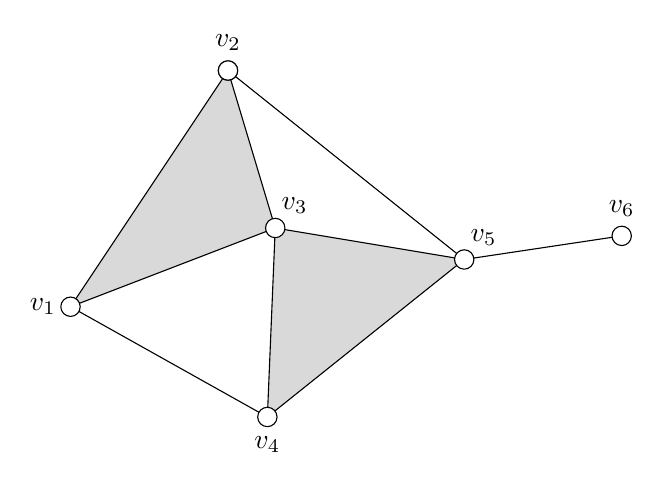
\begin{tikzpicture}[
    every node/.style={
      circle,
      draw=black,
      fill=white,
      inner sep=0pt,
      minimum size=7pt
    }
    ]

    \coordinate (v1) at (0,0);
    \coordinate (v2) at (2,3);
    \coordinate (v3) at (2.6,1);
    \coordinate (v4) at (2.5,-1.4);
    \coordinate (v5) at (5,.6);
    \coordinate (v6) at (7,.9);

    \draw[fill=gray!30!white] (v1) -- (v2) -- (v3) -- (v1) -- cycle;
    \draw[fill=gray!30!white] (v3) -- (v4) -- (v5) -- (v3) -- cycle;

    \draw (v1) -- (v4);
    \draw (v2) -- (v5);
    \draw (v5) -- (v6);

    \node (wv1) at (v1) {};
    \node (wv2) at (v2) {};
    \node (vv2) at (v2) {};
    \node (vv3) at (v3) {};
    \node (vv4) at (v4) {};
    \node (vv5) at (v5) {};
    \node (vv6) at (v6) {};

    \node[draw=none, xshift=-1em] (wv1) at (v1) {$v_1$};
    \node[draw=none, yshift=1em] (wv2) at (v2) {$v_2$};
    \node[draw=none, xshift=.7em, yshift=.8em] (wv3) at (v3) {$v_3$};
    \node[draw=none, yshift=-1em] (wv4) at (v4) {$v_4$};
    \node[draw=none, xshift=.7em, yshift=.8em] (wv5) at (v5) {$v_5$};
    \node[draw=none, yshift=1em] (wv6) at (v6) {$v_6$};
  \end{tikzpicture}
  \caption{Simplicial complex $K$}
  \label{fig:F1}
\end{figure}
\begin{solution}
  First, we redraw the simplicial complex as follows:
  \begin{figure}[H]
    \centering
    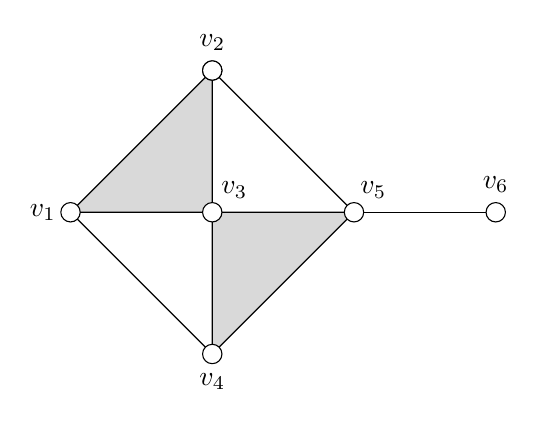
\begin{tikzpicture}[
      scale = .6,
      every node/.style={
        circle,
        draw=black,
        fill=white,
        inner sep=0pt,
        minimum size=7pt
      }
      ]

      \coordinate (v1) at (-3,0);
      \coordinate (v2) at (0,3);
      \coordinate (v3) at (0,0);
      \coordinate (v4) at (0,-3);
      \coordinate (v5) at (3,0);
      \coordinate (v6) at (6,0);

      \draw[fill=gray!30!white] (v1) -- (v2) -- (v3) -- (v1) -- cycle;
      \draw[fill=gray!30!white] (v3) -- (v4) -- (v5) -- (v3) -- cycle;

      \draw (v1) -- (v4);
      \draw (v2) -- (v5);
      \draw (v5) -- (v6);

      \node (wv1) at (v1) {};
      \node (wv2) at (v2) {};
      \node (vv2) at (v2) {};
      \node (vv3) at (v3) {};
      \node (vv4) at (v4) {};
      \node (vv5) at (v5) {};
      \node (vv6) at (v6) {};

      \node[draw=none, xshift=-1em] (wv1) at (v1) {$v_1$};
      \node[draw=none, yshift=1em] (wv2) at (v2) {$v_2$};
      \node[draw=none, xshift=.8em, yshift=.8em] (wv3) at (v3) {$v_3$};
      \node[draw=none, yshift=-1em] (wv4) at (v4) {$v_4$};
      \node[draw=none, xshift=.7em, yshift=.8em] (wv5) at (v5) {$v_5$};
      \node[draw=none, yshift=1em] (wv6) at (v6) {$v_6$};
    \end{tikzpicture}
    \caption{Simplicial complex $K$, straightened out}
  \end{figure}
  For the purposes of this problem, take angled brackets indicate span. We have
  \begin{enumerate}[label=(\roman*)]
  \item We calculate the $k=0$ case.
    \begin{enumerate}
    \item Elements of $\msf C_0(K)$ are formal linear combinations over the
      set $\set{v_1, v_2, \ldots, v_6}$. Then
      \[
        \msf C_0(K) = \ip[Big]{v_1, v_2, v_3, v_4, v_5, v_6}
      \]
      that is, collections of points in $\msf C_0(K)$.
    \item Let $\sigma_1, \ldots, \sigma_k \in \msf C_0(K).$ Then by definition,
      \begin{align*}
        \partial\pn{\sum_{i=1}^k \sigma_i}
        &= \sum_{i=1}^k \partial(\sigma_i)\\
        &= \sum_{i=1}^k 0 \\
        &= 0
      \end{align*}
      hence $\msf Z_n(K) = \msf C_n(K)$.
    \item A $\sigma \in \msf C_0(K)$ is an $n$-boundary if $\exists \tau \in
      \msf C_{1}(K)$ with $\partial(\tau) = \sigma$. Note, for any
      $1$-dimensional face $\set{v_iv_j} \in K$,
      \begin{align*}
        \partial(\set{v_iv_j})
        &= \set{v_i \widehat{v_j}} + \set{\widehat{v_i}v_j} \\
        &= \set{v_i} + \set{v_j} \\
        &= \delta_{ij}.
      \end{align*}
      Hence, any edge formed of a pair of two distinct vertices yields a
      nonempty boundary. We first count all edges:
      \begin{figure}[H]
        \centering
        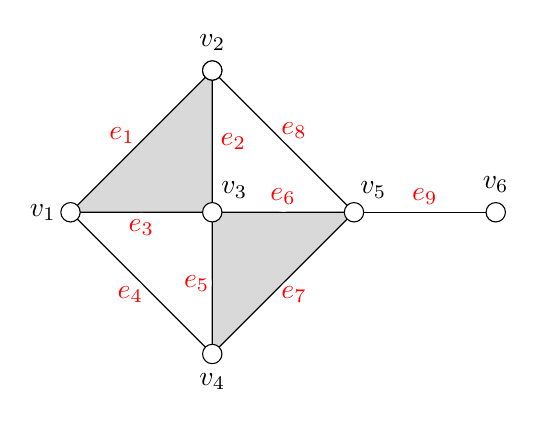
\begin{tikzpicture}[
          scale = .6,
          every node/.style={
            circle,
            draw=black,
            fill=white,
            inner sep=0pt,
            minimum size=7pt
          }
          ]

          \coordinate (v1) at (-3,0);
          \coordinate (v2) at (0,3);
          \coordinate (v3) at (0,0);
          \coordinate (v4) at (0,-3);
          \coordinate (v5) at (3,0);
          \coordinate (v6) at (6,0);

          \draw[fill=gray!30!white] (v1) -- (v2)
          % draw and label the edge between v1 and v2
          node[draw=none, midway, above left, xshift=-.3em, yshift=-.2em]
          {\color{red} $e_1$} -- (v3)
          % draw the edge between v2 and v3, and label it as well
          node[draw=none, midway, right, xshift=.2em] {\color{red} $e_2$}
          -- (v1)
          % draw the edge between v3 and v1, and label it as well
          node[draw=none, midway, below] {\color{red}$e_3$} -- cycle;

          \draw (v1) -- (v4) node[draw=none, midway, below left] {\color{red} $e_4$};

          \draw[fill=gray!30!white] (v3) -- (v4)
          % edge between v3 and and v4
          node[draw=none, midway, left] {\color{red} $e_5$} -- (v5)
          % edge
          node[draw=none, midway, below right] {\color{red}$e_7$} -- (v3)
          %
          node[draw=none, midway, above] {\color{red} $e_6$} -- cycle;


          \draw (v2) -- (v5) node[draw=none, midway, above right] {\color{red} $e_8$};
          \draw (v5) -- (v6) node[draw=none, midway, above] {\color{red} $e_9$};

          \node (wv1) at (v1) {};
          \node (wv2) at (v2) {};
          \node (vv2) at (v2) {};
          \node (vv3) at (v3) {};
          \node (vv4) at (v4) {};
          \node (vv5) at (v5) {};
          \node (vv6) at (v6) {};

          \node[draw=none, xshift=-1em] (wv1) at (v1) {$v_1$};
          \node[draw=none, yshift=1em] (wv2) at (v2) {$v_2$};
          \node[draw=none, xshift=.8em, yshift=.8em] (wv3) at (v3) {$v_3$};
          \node[draw=none, yshift=-1em] (wv4) at (v4) {$v_4$};
          \node[draw=none, xshift=.7em, yshift=.8em] (wv5) at (v5) {$v_5$};
          \node[draw=none, yshift=1em] (wv6) at (v6) {$v_6$};
        \end{tikzpicture}
        \caption{Simplicial complex $K$ with simple edges}
      \end{figure}
      Since $\msf B_0(K)$ is a subgroup of $\msf C_0(K)$, by closure under
      $+$, we see that any $v_i+v_j$ in $K$ such that there exists a path
      from $v_i$ to $v_j$ (when $K$ is considered a graph) is an element of
      $\msf B_0(K)$. In fact, we can say more:

      \textbf{Claim:} Since $K$ is connected as a graph, any even collection
      of vertices is in $\msf B_n(K)$.

      \textbf{Proof of Claim:} Suppose we have $\sigma = \set{v_{i_1}} +
      \set{v_{i_2}} + \cdots + \set{v_{i_{2k}}}$, where $k \in \NN$. Then
      for each $j = 1, \ldots, k$, let $\tau_j$ be a sum of edges representing
      a path from $v_{i_j}$ to $v_{i_{j+1}}$. For example, if $v_{i_j} =
      v_6$ and $v_{i_{j+1}} = v_2$, we could take the following approaches:
      \begin{figure}[H]
        \centering
        \begin{subfigure}{.49\linewidth}
          \centering
          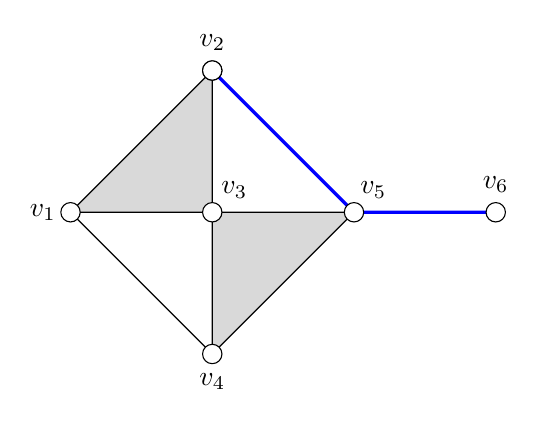
\begin{tikzpicture}[
            scale = .6,
            every node/.style={
              circle,
              draw=black,
              fill=white,
              inner sep=0pt,
              minimum size=7pt
            }
            ]

            \coordinate (v1) at (-3,0);
            \coordinate (v2) at (0,3);
            \coordinate (v3) at (0,0);
            \coordinate (v4) at (0,-3);
            \coordinate (v5) at (3,0);
            \coordinate (v6) at (6,0);

            \draw[fill=gray!30!white] (v1) -- (v2) -- (v3) -- (v1) -- cycle;
            \draw[fill=gray!30!white] (v3) -- (v4) -- (v5) -- (v3) -- cycle;

            \draw (v1) -- (v4);
            \draw (v2) -- (v5);
            \draw (v5) -- (v6);

            \draw[draw=blue, very thick] (v6) -- (v5) -- (v2);

            \node (wv1) at (v1) {};
            \node (wv2) at (v2) {};
            \node (vv2) at (v2) {};
            \node (vv3) at (v3) {};
            \node (vv4) at (v4) {};
            \node (vv5) at (v5) {};
            \node (vv6) at (v6) {};

            \node[draw=none, xshift=-1em] (wv1) at (v1) {$v_1$};
            \node[draw=none, yshift=1em] (wv2) at (v2) {$v_2$};
            \node[draw=none, xshift=.8em, yshift=.8em] (wv3) at (v3) {$v_3$};
            \node[draw=none, yshift=-1em] (wv4) at (v4) {$v_4$};
            \node[draw=none, xshift=.7em, yshift=.8em] (wv5) at (v5) {$v_5$};
            \node[draw=none, yshift=1em] (wv6) at (v6) {$v_6$};
          \end{tikzpicture}
        \end{subfigure}
        \begin{subfigure}{.49\linewidth}
          \centering
          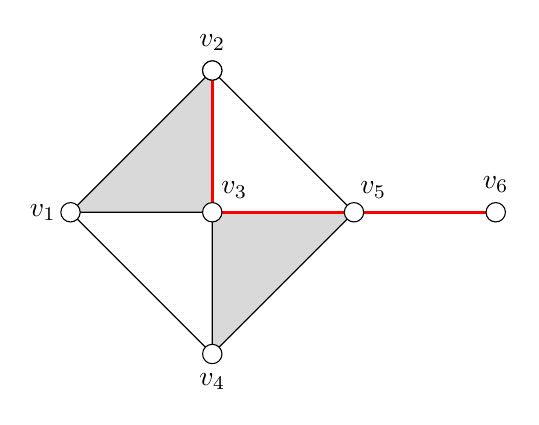
\begin{tikzpicture}[
            scale = .6,
            every node/.style={
              circle,
              draw=black,
              fill=white,
              inner sep=0pt,
              minimum size=7pt
            }
            ]

            \coordinate (v1) at (-3,0);
            \coordinate (v2) at (0,3);
            \coordinate (v3) at (0,0);
            \coordinate (v4) at (0,-3);
            \coordinate (v5) at (3,0);
            \coordinate (v6) at (6,0);

            \draw[fill=gray!30!white] (v1) -- (v2) -- (v3) -- (v1) -- cycle;
            \draw[fill=gray!30!white] (v3) -- (v4) -- (v5) -- (v3) -- cycle;

            \draw (v1) -- (v4);
            \draw (v2) -- (v5);
            \draw (v5) -- (v6);

            \draw[draw=red, very thick] (v6) -- (v5) -- (v3) -- (v2);

            \node (wv1) at (v1) {};
            \node (wv2) at (v2) {};
            \node (vv2) at (v2) {};
            \node (vv3) at (v3) {};
            \node (vv4) at (v4) {};
            \node (vv5) at (v5) {};
            \node (vv6) at (v6) {};

            \node[draw=none, xshift=-1em] (wv1) at (v1) {$v_1$};
            \node[draw=none, yshift=1em] (wv2) at (v2) {$v_2$};
            \node[draw=none, xshift=.8em, yshift=.8em] (wv3) at (v3) {$v_3$};
            \node[draw=none, yshift=-1em] (wv4) at (v4) {$v_4$};
            \node[draw=none, xshift=.7em, yshift=.8em] (wv5) at (v5) {$v_5$};
            \node[draw=none, yshift=1em] (wv6) at (v6) {$v_6$};
          \end{tikzpicture}
        \end{subfigure}
        \begin{subfigure}{.49\linewidth}
          \centering
          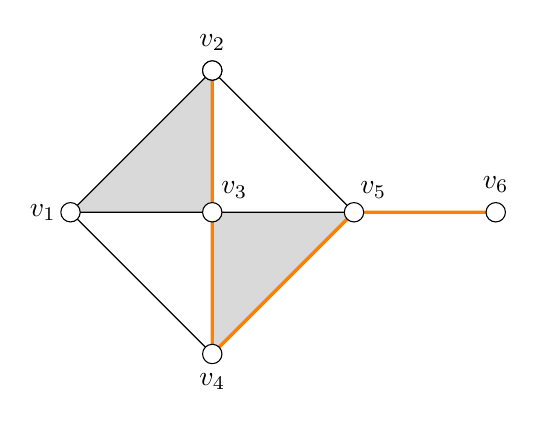
\begin{tikzpicture}[
            scale = .6,
            every node/.style={
              circle,
              draw=black,
              fill=white,
              inner sep=0pt,
              minimum size=7pt
            }
            ]

            \coordinate (v1) at (-3,0);
            \coordinate (v2) at (0,3);
            \coordinate (v3) at (0,0);
            \coordinate (v4) at (0,-3);
            \coordinate (v5) at (3,0);
            \coordinate (v6) at (6,0);

            \draw[fill=gray!30!white] (v1) -- (v2) -- (v3) -- (v1) -- cycle;
            \draw[fill=gray!30!white] (v3) -- (v4) -- (v5) -- (v3) -- cycle;

            \draw (v1) -- (v4);
            \draw (v2) -- (v5);
            \draw (v5) -- (v6);

            \draw[draw=orange, very thick] (v6) -- (v5) -- (v4) -- (v3)-- (v2);

            \node (wv1) at (v1) {};
            \node (wv2) at (v2) {};
            \node (vv2) at (v2) {};
            \node (vv3) at (v3) {};
            \node (vv4) at (v4) {};
            \node (vv5) at (v5) {};
            \node (vv6) at (v6) {};

            \node[draw=none, xshift=-1em] (wv1) at (v1) {$v_1$};
            \node[draw=none, yshift=1em] (wv2) at (v2) {$v_2$};
            \node[draw=none, xshift=.8em, yshift=.8em] (wv3) at (v3) {$v_3$};
            \node[draw=none, yshift=-1em] (wv4) at (v4) {$v_4$};
            \node[draw=none, xshift=.7em, yshift=.8em] (wv5) at (v5) {$v_5$};
            \node[draw=none, yshift=1em] (wv6) at (v6) {$v_6$};
          \end{tikzpicture}
        \end{subfigure}
        \begin{subfigure}{.49\linewidth}
          \centering
          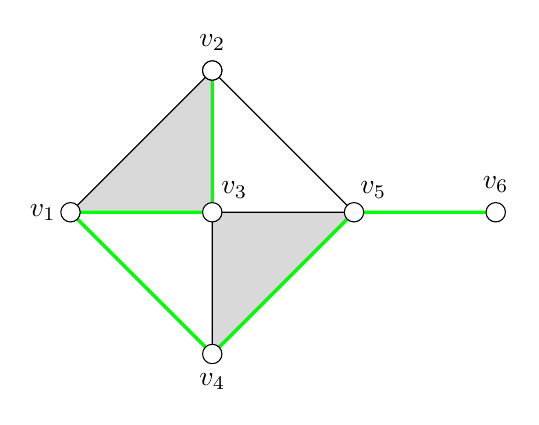
\begin{tikzpicture}[
            scale = .6,
            every node/.style={
              circle,
              draw=black,
              fill=white,
              inner sep=0pt,
              minimum size=7pt
            }
            ]

            \coordinate (v1) at (-3,0);
            \coordinate (v2) at (0,3);
            \coordinate (v3) at (0,0);
            \coordinate (v4) at (0,-3);
            \coordinate (v5) at (3,0);
            \coordinate (v6) at (6,0);

            \draw[fill=gray!30!white] (v1) -- (v2) -- (v3) -- (v1) -- cycle;
            \draw[fill=gray!30!white] (v3) -- (v4) -- (v5) -- (v3) -- cycle;

            \draw (v1) -- (v4);
            \draw (v2) -- (v5);
            \draw (v5) -- (v6);

            \draw[draw=green, very thick] (v6) -- (v5) -- (v4) -- (v1) -- (v3) -- (v2);

            \node (wv1) at (v1) {};
            \node (wv2) at (v2) {};
            \node (vv2) at (v2) {};
            \node (vv3) at (v3) {};
            \node (vv4) at (v4) {};
            \node (vv5) at (v5) {};
            \node (vv6) at (v6) {};

            \node[draw=none, xshift=-1em] (wv1) at (v1) {$v_1$};
            \node[draw=none, yshift=1em] (wv2) at (v2) {$v_2$};
            \node[draw=none, xshift=.8em, yshift=.8em] (wv3) at (v3) {$v_3$};
            \node[draw=none, yshift=-1em] (wv4) at (v4) {$v_4$};
            \node[draw=none, xshift=.7em, yshift=.8em] (wv5) at (v5) {$v_5$};
            \node[draw=none, yshift=1em] (wv6) at (v6) {$v_6$};
          \end{tikzpicture}
        \end{subfigure}
      \end{figure}\clearpage
      \begin{figure}[H]\ContinuedFloat
        \begin{subfigure}{.49\linewidth}
          \centering
          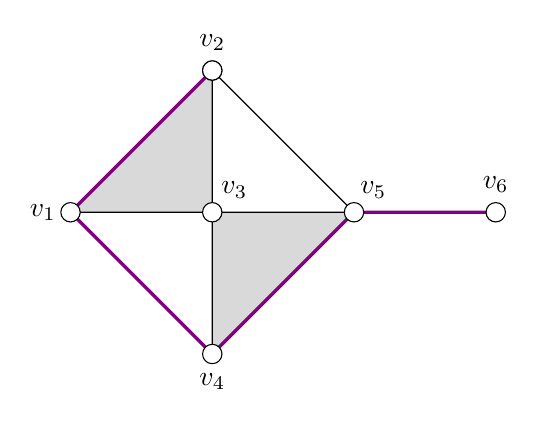
\begin{tikzpicture}[
            scale = .6,
            every node/.style={
              circle,
              draw=black,
              fill=white,
              inner sep=0pt,
              minimum size=7pt
            }
            ]

            \coordinate (v1) at (-3,0);
            \coordinate (v2) at (0,3);
            \coordinate (v3) at (0,0);
            \coordinate (v4) at (0,-3);
            \coordinate (v5) at (3,0);
            \coordinate (v6) at (6,0);

            \draw[fill=gray!30!white] (v1) -- (v2) -- (v3) -- (v1) -- cycle;
            \draw[fill=gray!30!white] (v3) -- (v4) -- (v5) -- (v3) -- cycle;

            \draw (v1) -- (v4);
            \draw (v2) -- (v5);
            \draw (v5) -- (v6);

            \draw[draw=violet, very thick] (v6) -- (v5) -- (v4) -- (v1)-- (v2);

            \node (wv1) at (v1) {};
            \node (wv2) at (v2) {};
            \node (vv2) at (v2) {};
            \node (vv3) at (v3) {};
            \node (vv4) at (v4) {};
            \node (vv5) at (v5) {};
            \node (vv6) at (v6) {};

            \node[draw=none, xshift=-1em] (wv1) at (v1) {$v_1$};
            \node[draw=none, yshift=1em] (wv2) at (v2) {$v_2$};
            \node[draw=none, xshift=.8em, yshift=.8em] (wv3) at (v3) {$v_3$};
            \node[draw=none, yshift=-1em] (wv4) at (v4) {$v_4$};
            \node[draw=none, xshift=.7em, yshift=.8em] (wv5) at (v5) {$v_5$};
            \node[draw=none, yshift=1em] (wv6) at (v6) {$v_6$};
          \end{tikzpicture}
        \end{subfigure}
        \begin{subfigure}{.49\linewidth}
          \centering
          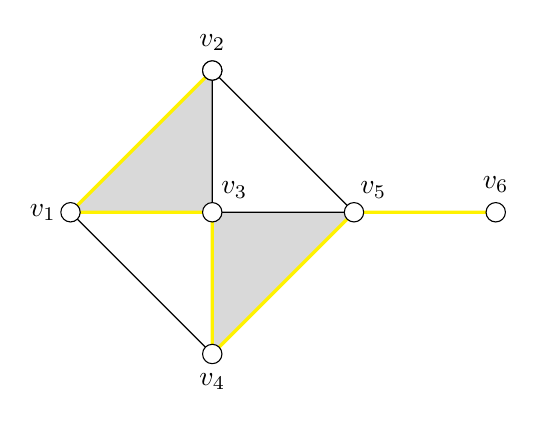
\begin{tikzpicture}[
            scale = .6,
            every node/.style={
              circle,
              draw=black,
              fill=white,
              inner sep=0pt,
              minimum size=7pt
            }
            ]

            \coordinate (v1) at (-3,0);
            \coordinate (v2) at (0,3);
            \coordinate (v3) at (0,0);
            \coordinate (v4) at (0,-3);
            \coordinate (v5) at (3,0);
            \coordinate (v6) at (6,0);

            \draw[fill=gray!30!white] (v1) -- (v2) -- (v3) -- (v1) -- cycle;
            \draw[fill=gray!30!white] (v3) -- (v4) -- (v5) -- (v3) -- cycle;

            \draw (v1) -- (v4);
            \draw (v2) -- (v5);
            \draw (v5) -- (v6);

            \draw[draw=yellow, very thick] (v6) -- (v5) -- (v4) -- (v3) -- (v1) -- (v2);

            \node (wv1) at (v1) {};
            \node (wv2) at (v2) {};
            \node (vv2) at (v2) {};
            \node (vv3) at (v3) {};
            \node (vv4) at (v4) {};
            \node (vv5) at (v5) {};
            \node (vv6) at (v6) {};

            \node[draw=none, xshift=-1em] (wv1) at (v1) {$v_1$};
            \node[draw=none, yshift=1em] (wv2) at (v2) {$v_2$};
            \node[draw=none, xshift=.8em, yshift=.8em] (wv3) at (v3) {$v_3$};
            \node[draw=none, yshift=-1em] (wv4) at (v4) {$v_4$};
            \node[draw=none, xshift=.7em, yshift=.8em] (wv5) at (v5) {$v_5$};
            \node[draw=none, yshift=1em] (wv6) at (v6) {$v_6$};
          \end{tikzpicture}
        \end{subfigure}
        \caption{Some paths from $v_6$ to $v_2$}
      \end{figure}
      among others. Taking the sum of the constituent edges in each path
      yields a sum of $1$-simplices with boundary $v_6,
      v_2$.\footnote{Justification: note that the coefficient on any given
        vertex when we apply $\partial$ is the degree of the vertex in our
        path. Hence, only the initial and terminal vertex don't get mapped
        to $0$.}
    \item Since $\msf B_n(K)$ is the group of all collections of even
      vertices in $\msf C_n(K)$, we have $\msf H_n(K) = \msf C_n(K)/\msf
      B_n(K) \cong \zmod{2}$.
    \end{enumerate}
  \item Now, we calculate the $k=1$ case.
    \begin{enumerate}
    \item Elements of $\msf C_1(K)$ are collections of linear combinations
      of the edges
      \[
        \msf C_1(K) = \ip{e_1, e_2, e_3, e_4, e_5, e_6, e_7, e_8, e_9}
      \]
    \item Elements of $\msf Z_1(K)$ are collections of edges such that
      each vertex contained in an edge in the collection has even degree.
      This corresponds to cyclic subgraphs of $K$ (as well as the empty
      cycle), e.g.:
      \begin{figure}[H]
        \centering
        \begin{subfigure}{.49\linewidth}
          \centering
          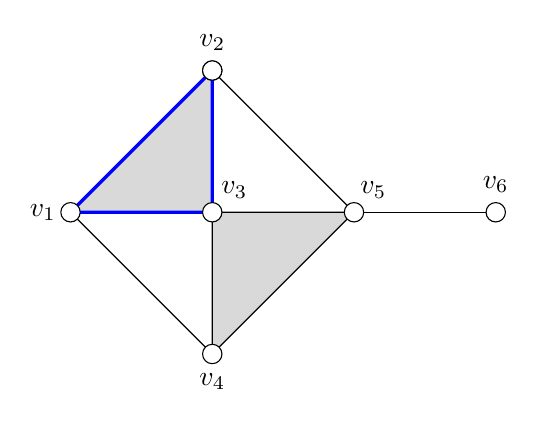
\begin{tikzpicture}[
            scale = .6,
            every node/.style={
              circle,
              draw=black,
              fill=white,
              inner sep=0pt,
              minimum size=7pt
            }
            ]

            \coordinate (v1) at (-3,0);
            \coordinate (v2) at (0,3);
            \coordinate (v3) at (0,0);
            \coordinate (v4) at (0,-3);
            \coordinate (v5) at (3,0);
            \coordinate (v6) at (6,0);

            \draw[fill=gray!30!white] (v1) -- (v2) -- (v3) -- (v1) -- cycle;
            \draw[fill=gray!30!white] (v3) -- (v4) -- (v5) -- (v3) -- cycle;

            \draw (v1) -- (v4);
            \draw (v2) -- (v5);
            \draw (v5) -- (v6);

            \draw[draw=blue, very thick] (v1) -- (v2) -- (v3) -- cycle;

            \node (wv1) at (v1) {};
            \node (wv2) at (v2) {};
            \node (vv2) at (v2) {};
            \node (vv3) at (v3) {};
            \node (vv4) at (v4) {};
            \node (vv5) at (v5) {};
            \node (vv6) at (v6) {};

            \node[draw=none, xshift=-1em] (wv1) at (v1) {$v_1$};
            \node[draw=none, yshift=1em] (wv2) at (v2) {$v_2$};
            \node[draw=none, xshift=.8em, yshift=.8em] (wv3) at (v3) {$v_3$};
            \node[draw=none, yshift=-1em] (wv4) at (v4) {$v_4$};
            \node[draw=none, xshift=.7em, yshift=.8em] (wv5) at (v5) {$v_5$};
            \node[draw=none, yshift=1em] (wv6) at (v6) {$v_6$};
          \end{tikzpicture}
        \end{subfigure}
        \begin{subfigure}{.49\linewidth}
          \centering
          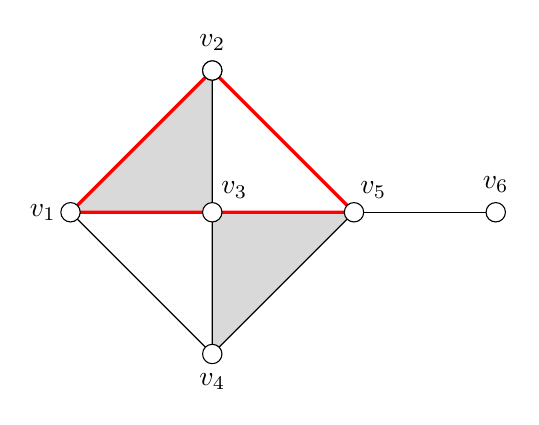
\begin{tikzpicture}[
            scale = .6,
            every node/.style={
              circle,
              draw=black,
              fill=white,
              inner sep=0pt,
              minimum size=7pt
            }
            ]

            \coordinate (v1) at (-3,0);
            \coordinate (v2) at (0,3);
            \coordinate (v3) at (0,0);
            \coordinate (v4) at (0,-3);
            \coordinate (v5) at (3,0);
            \coordinate (v6) at (6,0);

            \draw[fill=gray!30!white] (v1) -- (v2) -- (v3) -- (v1) -- cycle;
            \draw[fill=gray!30!white] (v3) -- (v4) -- (v5) -- (v3) -- cycle;

            \draw (v1) -- (v4);
            \draw (v2) -- (v5);
            \draw (v5) -- (v6);

            \draw[draw=red, very thick] (v1) -- (v2) -- (v5) -- (v3) -- (v1);

            \node (wv1) at (v1) {};
            \node (wv2) at (v2) {};
            \node (vv2) at (v2) {};
            \node (vv3) at (v3) {};
            \node (vv4) at (v4) {};
            \node (vv5) at (v5) {};
            \node (vv6) at (v6) {};

            \node[draw=none, xshift=-1em] (wv1) at (v1) {$v_1$};
            \node[draw=none, yshift=1em] (wv2) at (v2) {$v_2$};
            \node[draw=none, xshift=.8em, yshift=.8em] (wv3) at (v3) {$v_3$};
            \node[draw=none, yshift=-1em] (wv4) at (v4) {$v_4$};
            \node[draw=none, xshift=.7em, yshift=.8em] (wv5) at (v5) {$v_5$};
            \node[draw=none, yshift=1em] (wv6) at (v6) {$v_6$};
          \end{tikzpicture}
        \end{subfigure}
      \end{figure}
      \clearpage
      \begin{figure}[H]\ContinuedFloat
        \begin{subfigure}{.49\linewidth}
          \centering
          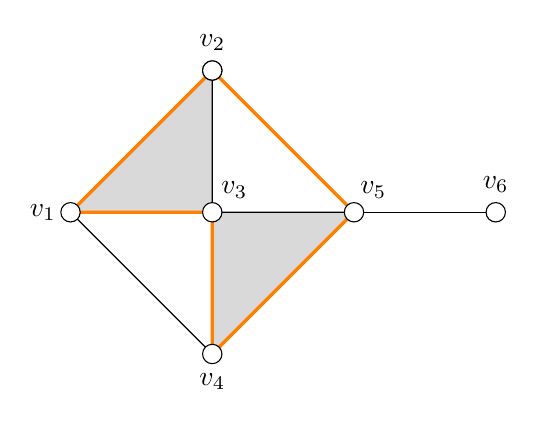
\begin{tikzpicture}[
            scale = .6,
            every node/.style={
              circle,
              draw=black,
              fill=white,
              inner sep=0pt,
              minimum size=7pt
            }
            ]

            \coordinate (v1) at (-3,0);
            \coordinate (v2) at (0,3);
            \coordinate (v3) at (0,0);
            \coordinate (v4) at (0,-3);
            \coordinate (v5) at (3,0);
            \coordinate (v6) at (6,0);

            \draw[fill=gray!30!white] (v1) -- (v2) -- (v3) -- (v1) -- cycle;
            \draw[fill=gray!30!white] (v3) -- (v4) -- (v5) -- (v3) -- cycle;

            \draw (v1) -- (v4);
            \draw (v2) -- (v5);
            \draw (v5) -- (v6);

            \draw[draw=orange, very thick] (v1) -- (v2) -- (v5) -- (v4)-- (v3) -- cycle;

            \node (wv1) at (v1) {};
            \node (wv2) at (v2) {};
            \node (vv2) at (v2) {};
            \node (vv3) at (v3) {};
            \node (vv4) at (v4) {};
            \node (vv5) at (v5) {};
            \node (vv6) at (v6) {};

            \node[draw=none, xshift=-1em] (wv1) at (v1) {$v_1$};
            \node[draw=none, yshift=1em] (wv2) at (v2) {$v_2$};
            \node[draw=none, xshift=.8em, yshift=.8em] (wv3) at (v3) {$v_3$};
            \node[draw=none, yshift=-1em] (wv4) at (v4) {$v_4$};
            \node[draw=none, xshift=.7em, yshift=.8em] (wv5) at (v5) {$v_5$};
            \node[draw=none, yshift=1em] (wv6) at (v6) {$v_6$};
          \end{tikzpicture}
        \end{subfigure}
        \begin{subfigure}{.49\linewidth}
          \centering
          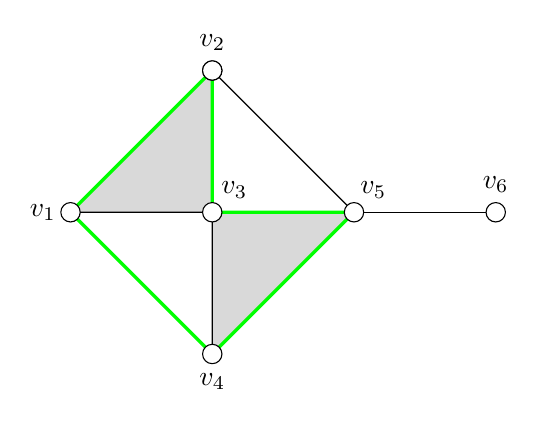
\begin{tikzpicture}[
            scale = .6,
            every node/.style={
              circle,
              draw=black,
              fill=white,
              inner sep=0pt,
              minimum size=7pt
            }
            ]

            \coordinate (v1) at (-3,0);
            \coordinate (v2) at (0,3);
            \coordinate (v3) at (0,0);
            \coordinate (v4) at (0,-3);
            \coordinate (v5) at (3,0);
            \coordinate (v6) at (6,0);

            \draw[fill=gray!30!white] (v1) -- (v2) -- (v3) -- (v1) -- cycle;
            \draw[fill=gray!30!white] (v3) -- (v4) -- (v5) -- (v3) -- cycle;

            \draw (v1) -- (v4);
            \draw (v2) -- (v5);
            \draw (v5) -- (v6);

            \draw[draw=green, very thick] (v1) -- (v2) -- (v3) -- (v5) -- (v4) -- cycle;

            \node (wv1) at (v1) {};
            \node (wv2) at (v2) {};
            \node (vv2) at (v2) {};
            \node (vv3) at (v3) {};
            \node (vv4) at (v4) {};
            \node (vv5) at (v5) {};
            \node (vv6) at (v6) {};

            \node[draw=none, xshift=-1em] (wv1) at (v1) {$v_1$};
            \node[draw=none, yshift=1em] (wv2) at (v2) {$v_2$};
            \node[draw=none, xshift=.8em, yshift=.8em] (wv3) at (v3) {$v_3$};
            \node[draw=none, yshift=-1em] (wv4) at (v4) {$v_4$};
            \node[draw=none, xshift=.7em, yshift=.8em] (wv5) at (v5) {$v_5$};
            \node[draw=none, yshift=1em] (wv6) at (v6) {$v_6$};
          \end{tikzpicture}
        \end{subfigure}
        \begin{subfigure}{.49\linewidth}
          \centering
          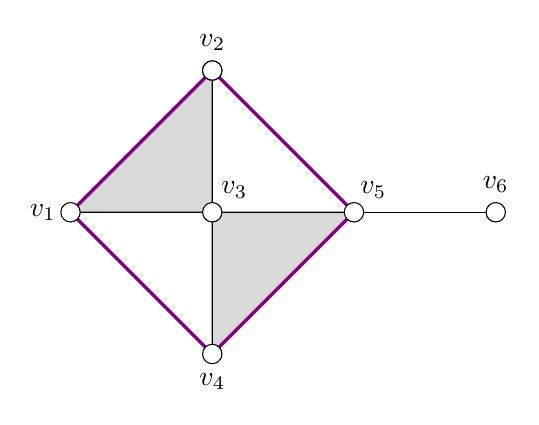
\begin{tikzpicture}[
            scale = .6,
            every node/.style={
              circle,
              draw=black,
              fill=white,
              inner sep=0pt,
              minimum size=7pt
            }
            ]

            \coordinate (v1) at (-3,0);
            \coordinate (v2) at (0,3);
            \coordinate (v3) at (0,0);
            \coordinate (v4) at (0,-3);
            \coordinate (v5) at (3,0);
            \coordinate (v6) at (6,0);

            \draw[fill=gray!30!white] (v1) -- (v2) -- (v3) -- (v1) -- cycle;
            \draw[fill=gray!30!white] (v3) -- (v4) -- (v5) -- (v3) -- cycle;

            \draw (v1) -- (v4);
            \draw (v2) -- (v5);
            \draw (v5) -- (v6);

            \draw[draw=violet, very thick] (v1) -- (v2) -- (v5) -- (v4) -- cycle;

            \node (wv1) at (v1) {};
            \node (wv2) at (v2) {};
            \node (vv2) at (v2) {};
            \node (vv3) at (v3) {};
            \node (vv4) at (v4) {};
            \node (vv5) at (v5) {};
            \node (vv6) at (v6) {};

            \node[draw=none, xshift=-1em] (wv1) at (v1) {$v_1$};
            \node[draw=none, yshift=1em] (wv2) at (v2) {$v_2$};
            \node[draw=none, xshift=.8em, yshift=.8em] (wv3) at (v3) {$v_3$};
            \node[draw=none, yshift=-1em] (wv4) at (v4) {$v_4$};
            \node[draw=none, xshift=.7em, yshift=.8em] (wv5) at (v5) {$v_5$};
            \node[draw=none, yshift=1em] (wv6) at (v6) {$v_6$};
          \end{tikzpicture}
        \end{subfigure}
        \begin{subfigure}{.49\linewidth}
          \centering
          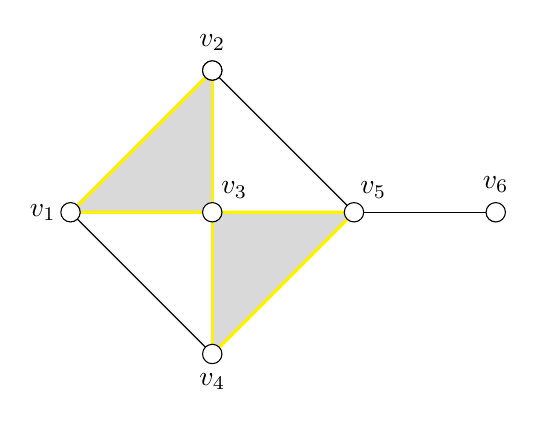
\begin{tikzpicture}[
            scale = .6,
            every node/.style={
              circle,
              draw=black,
              fill=white,
              inner sep=0pt,
              minimum size=7pt
            }
            ]

            \coordinate (v1) at (-3,0);
            \coordinate (v2) at (0,3);
            \coordinate (v3) at (0,0);
            \coordinate (v4) at (0,-3);
            \coordinate (v5) at (3,0);
            \coordinate (v6) at (6,0);

            \draw[fill=gray!30!white] (v1) -- (v2) -- (v3) -- (v1) -- cycle;
            \draw[fill=gray!30!white] (v3) -- (v4) -- (v5) -- (v3) -- cycle;

            \draw (v1) -- (v4);
            \draw (v2) -- (v5);
            \draw (v5) -- (v6);

            \draw[draw=yellow, very thick] (v1) -- (v2) -- (v3) -- cycle;
            \draw[draw=yellow, very thick] (v3) -- (v4) -- (v5) -- cycle;

            \node (wv1) at (v1) {};
            \node (wv2) at (v2) {};
            \node (vv2) at (v2) {};
            \node (vv3) at (v3) {};
            \node (vv4) at (v4) {};
            \node (vv5) at (v5) {};
            \node (vv6) at (v6) {};

            \node[draw=none, xshift=-1em] (wv1) at (v1) {$v_1$};
            \node[draw=none, yshift=1em] (wv2) at (v2) {$v_2$};
            \node[draw=none, xshift=.8em, yshift=.8em] (wv3) at (v3) {$v_3$};
            \node[draw=none, yshift=-1em] (wv4) at (v4) {$v_4$};
            \node[draw=none, xshift=.7em, yshift=.8em] (wv5) at (v5) {$v_5$};
            \node[draw=none, yshift=1em] (wv6) at (v6) {$v_6$};
          \end{tikzpicture}
        \end{subfigure}
        \caption{Some cycles in $K$}
      \end{figure}
    \item First, consider the following diagram:
      \begin{figure}[H]
        \centering
        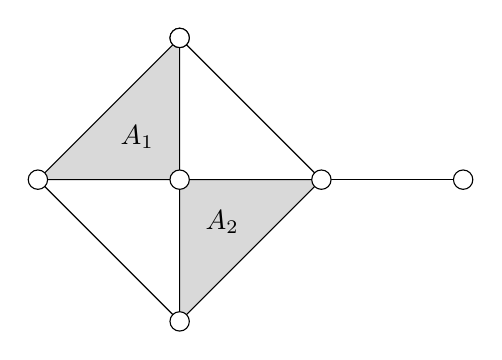
\begin{tikzpicture}[
          scale = .6,
          every node/.style={
            circle,
            draw=black,
            fill=white,
            inner sep=0pt,
            minimum size=7pt
          }
          ]

          \coordinate (v1) at (-3,0);
          \coordinate (v2) at (0,3);
          \coordinate (v3) at (0,0);
          \coordinate (v4) at (0,-3);
          \coordinate (v5) at (3,0);
          \coordinate (v6) at (6,0);

          \draw[fill=gray!30!white] (v1) -- (v2) -- (v3) -- (v1) -- cycle;

          \draw (v1) -- (v4);

          \draw[fill=gray!30!white] (v3) -- (v4) -- (v5) -- (v3) -- cycle;


          \draw (v2) -- (v5) ;
          \draw (v5) -- (v6) ;

          \node (wv1) at (v1) {};
          \node (wv2) at (v2) {};
          \node (vv2) at (v2) {};
          \node (vv3) at (v3) {};
          \node (vv4) at (v4) {};
          \node (vv5) at (v5) {};
          \node (vv6) at (v6) {};

          \node[draw=none,fill=none] (a1) at (-.9,.9) {$A_1$};
          \node[draw=none,fill=none] (a1) at (.9,-.9) {$A_2$};
        \end{tikzpicture}
        \caption{Two $n=2$ simplices}
      \end{figure}
      $\mb 0_1$ bounds $\mb 0_2$. Since $\partial(A_1) \cap \partial(A_2) =
      \varnothing$, then the other two cycles in $\msf B_1(K)$ are just
      $\partial(A_1)$ and $\partial(A_2)$, respectively.
    \item $\msf H_1(K) \cong \zmod{2} \times \zmod{2}$ (equivalence classes
      have representative elements $\mb 0, \partial(A_1), \partial(A_2),
      \partial(A_1) + \partial(A_2)$)
    \end{enumerate}
  \item For $k=2$, we have
    \begin{enumerate}
    \item $\msf C_2(K) \cong \zmod{2} \times \zmod{2}$
    \item $\msf Z_2(K) \cong \mb 0$
    \item $\msf B_2(K) \cong \mb 0$
    \item And hence $\msf H_2(K) \cong \mb 0$.
    \end{enumerate}
  \end{enumerate}
\end{solution}
\begin{problem}[16.7]
  If $K$ is a one-point space, $\msf H_n(K) \cong 0$ for $n \geq 0$, and $\msf
  H_0(K) \cong \zmod{2}$.
\end{problem}
\begin{solution}
  For $n > 0$, $\msf C_n(K)$ is the trivial group. Since $\msf Z_n(K) \leq \msf
  C_n(K)$, we thus have $\msf Z_n(K) \cong 0$, and so $\msf H_n(K) \cong 0$.

  For the $n = 0$, note that $\msf Z_0(K) = \msf C_0(K) \cong \zmod{2}$ (every
  point is definitionally a 0-cycle). Since $K$ contains no 1-simplices, $\msf
  B_0(K) = \mb 0$, hence $\msf H_0(K) \cong \zmod{2}$.
\end{solution}
\begin{definition}[Acyclic]
  Any space with the homology groups of a point is called \emph{acyclic}.
\end{definition}
\begin{definition}[Simplicially connected]
  Let $K$ be a simplicial complex. Then we call $K$ \emph{simplicially
    connected} iff for all pairs of 0-simplices $v_0, v_n \in K$, there exists a
  sequence of 0-simplices $\set{v_i}_{i\in [n]}$ such that for all $i \in [n]$
  (with $i \neq n$), $\set{v_iv_{i+1}}$ is a 1-simplex in $K$. Note, this
  corresponds exactly to $K$ being connected as a graph, where the 0-simplices
  represent vertices, and the 1-simplices represent edges.
\end{definition}
\begin{problem}[16.8]
  If $K$ is simplicially connected, then $\msf H_0(K) \cong \zmod{2}$. If $K$
  has $r$ simplicially connected components, then
  \[
    \msf H_0(K)\cong \prod_{i=1}^r \zmod{2}
  \]
\end{problem}
\begin{solution}
  \begin{enumerate}
  \item Suppose $K$ is simplicially connected. We want to show $\msf H_0(K)
    \cong \zmod{2}$. First, observe that $\msf Z_0(K) \cong \msf C_0(K)$
    (every 0 simplex has trivial boundary). By properties of module
    homomorphisms, for all $\sigma \in \msf B_0(K)$, $\sigma$ is a basis
    element of $\msf B_0(K)$ iff $\exists \tau \in \msf C_1(K)$ such that
    $\tau$ is a basis element of $\msf C_1(K)$, and $\partial_1(\tau) =
    \sigma$. Thus, $\msf B_0(K)$ is spanned by $\set{\set{\set{v_i} +
        \set{v_j}} \MID \set{v_iv_j} \in K}$. It follows that $\msf B_0(K)$
    contains exactly those elements of $\msf C_0(K)$ with an even number of
    vertices.\footnote{Since $\msf B_0(K)$ is generated by pairs.}

    It follows that $\msf H_0(K) = \msf Z_0(K)/\msf B_0(K) \cong \zmod{2}$
    (any $0$-chain has either an even or odd number of vertices).
  \item This follows by applying the above argument to each of the connected
    components.
  \end{enumerate}
\end{solution}
\begin{problem}[16.9]
  Let $K$ be a triangulation of a $3$-dimensional ball that consists of a
  3-simplex together with its faces. Compute $\msf H_n(K)$ for each $n$.
\end{problem}
\begin{solution}
  \begin{figure}[H]
    \centering
    \begin{subfigure}{\linewidth}
      \centering
      \tdplotsetmaincoords{70}{80}
      \begin{tikzpicture}[tdplot_main_coords,scale=2]
        \path
        coordinate (A) at (0,0,0)
        coordinate (B) at (2,0,0)
        coordinate (C) at (1,1.732,0)
        coordinate (D) at (1,.577,1.733);

        \draw [dashed] (A)--(C);
        \fill [opacity=.5, red!30!white] (A) -- (B) -- (C) -- cycle;
        \fill [opacity=.5, blue!30!white] (D) -- (B) -- (A) -- cycle;
        \fill [opacity=.5, green!30!white] (D) -- (A) -- (C) -- cycle;
        \draw[thick] (A) -- (B) (A) -- (D);
        \draw[thick, fill opacity=.5, fill=orange!30!white] (D) -- (B) -- (C) -- cycle;

        \node (V) at (1,.577,.433) {\LARGE $V_1$};

        \foreach \v/\position in {A/left,B/below,C/right,D/above} {
          \draw[fill=black] (\v) circle (0.5pt) node [\position=0.2mm] {$\v$};
        }
      \end{tikzpicture}
    \end{subfigure}\\\vspace{1cm}
    \begin{subfigure}{.24\linewidth}
      \centering
      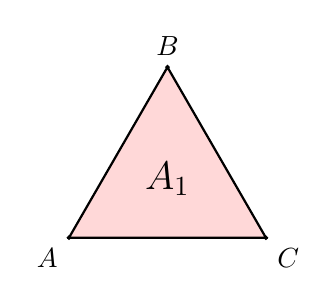
\begin{tikzpicture}[scale=1.25]
        \path
        coordinate (A) at (0,0)
        coordinate (C) at (2,0)
        coordinate (B) at (1,1.732);

        \draw[thick, fill opacity=.5, fill=red!30!white] (A) -- (B) -- (C) -- cycle;

        \node (A1) at (1,.6) {\Large $A_1$};

        \foreach \v/\position in {A/below left, C/below right, B/above} {
          \draw[fill=black] (\v) circle (0.5pt) node [\position=0.2mm] {$\v$};
        }
      \end{tikzpicture}
    \end{subfigure}
    \begin{subfigure}{.24\linewidth}
      \centering
      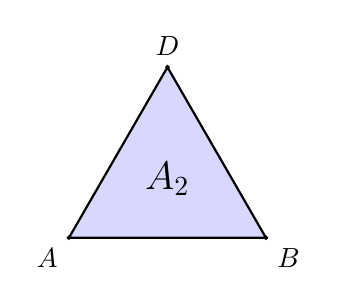
\begin{tikzpicture}[scale=1.25]
        \path
        coordinate (A) at (0,0)
        coordinate (B) at (2,0)
        coordinate (D) at (1,1.732);

        \draw[thick, fill opacity=.5, fill=blue!30!white] (D) -- (B) -- (A) -- cycle;

        \node (A2) at (1,.6) {\Large $A_2$};

        \foreach \v/\position in {A/below left, B/below right, D/above} {
          \draw[fill=black] (\v) circle (0.5pt) node [\position=0.2mm] {$\v$};
        }
      \end{tikzpicture}
    \end{subfigure}
    \begin{subfigure}{.24\linewidth}
      \centering
      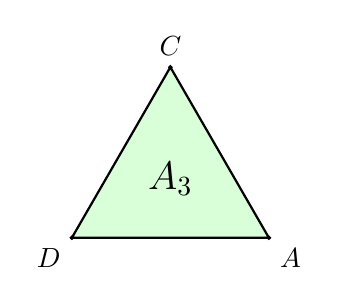
\begin{tikzpicture}[scale=1.25]
        \path
        coordinate (D) at (0,0)
        coordinate (A) at (2,0)
        coordinate (C) at (1,1.732);

        \draw[thick, fill opacity=.5, fill=green!30!white] (D) -- (A) -- (C) -- cycle;

        \node (A3) at (1,.6) {\Large $A_3$};

        \foreach \v/\position in {D/below left, A/below right, C/above} {
          \draw[fill=black] (\v) circle (0.5pt) node [\position=0.2mm] {$\v$};
        }
      \end{tikzpicture}
    \end{subfigure}
    \begin{subfigure}{.24\linewidth}
      \centering
      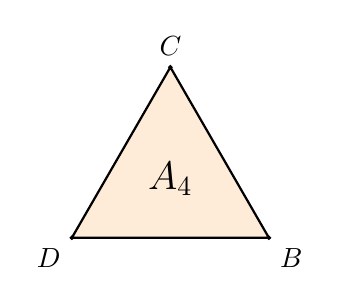
\begin{tikzpicture}[scale=1.25]
        \path
        coordinate (D) at (0,0)
        coordinate (B) at (2,0)
        coordinate (C) at (1,1.732);

        \draw[thick, fill opacity=.5, fill=orange!30!white] (D) -- (B) -- (C) -- cycle;

        \node (A4) at (1,.6) {\Large $A_4$};

        \foreach \v/\position in {D/below left, B/below right, C/above} {
          \draw[fill=black] (\v) circle (0.5pt) node [\position=0.2mm] {$\v$};
        }
      \end{tikzpicture}
    \end{subfigure}\\\vspace{1cm}
    \tikzset{
      brace/.style={
        thick,
        decoration={brace, mirror, raise=1pt, amplitude=6pt},
        decorate
      },
      blabel/.style={
        right, pos=.5, xshift=7pt, yshift=-2pt
      }
    }
    \begin{subfigure}{.161\linewidth}
      \centering
      \begin{tikzpicture}[scale=1.25]
        \def\firstcoord{A}
        \def\secondcoord{B}
        \path coordinate (\firstcoord) at (0,0) coordinate (\secondcoord) at (0,1.73);
        \draw[thick] (\firstcoord) -- (\secondcoord);

        \draw[brace] (.3,-.4) -- node[blabel] {\Large $e_1$} (.3,2.13);

        \foreach \v/\position in {\firstcoord/below, \secondcoord/above} {
          \draw[fill=black] (\v) circle (0.5pt) node [\position=0.2mm] {$\v$};
        }
      \end{tikzpicture}
    \end{subfigure}
    \begin{subfigure}{.161\linewidth}
      \centering
      \begin{tikzpicture}[scale=1.25]
        \def\firstcoord{A}
        \def\secondcoord{C}
        \path coordinate (\firstcoord) at (0,0) coordinate (\secondcoord) at (0,1.73);
        \draw[thick] (\firstcoord) -- (\secondcoord);

        \draw[brace] (.3,-.4) -- node[blabel] {\Large $e_2$} (.3,2.13);

        \foreach \v/\position in {\firstcoord/below, \secondcoord/above} {
          \draw[fill=black] (\v) circle (0.5pt) node [\position=0.2mm] {$\v$};
        }
      \end{tikzpicture}
    \end{subfigure}
    \begin{subfigure}{.161\linewidth}
      \centering
      \begin{tikzpicture}[scale=1.25]
        \def\firstcoord{A}
        \def\secondcoord{D}
        \path coordinate (\firstcoord) at (0,0) coordinate (\secondcoord) at (0,1.73);
        \draw[thick] (\firstcoord) -- (\secondcoord);

        \draw[brace] (.3,-.4) -- node[blabel] {\Large $e_3$} (.3,2.13);

        \foreach \v/\position in {\firstcoord/below, \secondcoord/above} {
          \draw[fill=black] (\v) circle (0.5pt) node [\position=0.2mm] {$\v$};
        }
      \end{tikzpicture}
    \end{subfigure}
    \begin{subfigure}{.161\linewidth}
      \centering
      \begin{tikzpicture}[scale=1.25]
        \def\firstcoord{B}
        \def\secondcoord{C}
        \path coordinate (\firstcoord) at (0,0) coordinate (\secondcoord) at (0,1.73);
        \draw[thick] (\firstcoord) -- (\secondcoord);

        \draw[brace] (.3,-.4) -- node[blabel] {\Large $e_4$} (.3,2.13);

        \foreach \v/\position in {\firstcoord/below, \secondcoord/above} {
          \draw[fill=black] (\v) circle (0.5pt) node [\position=0.2mm] {$\v$};
        }
      \end{tikzpicture}
    \end{subfigure}
    \begin{subfigure}{.161\linewidth}
      \centering
      \begin{tikzpicture}[scale=1.25]
        \def\firstcoord{B}
        \def\secondcoord{D}
        \path coordinate (\firstcoord) at (0,0) coordinate (\secondcoord) at (0,1.73);
        \draw[thick] (\firstcoord) -- (\secondcoord);

        \draw[brace] (.3,-.4) -- node[blabel] {\Large $e_5$} (.3,2.13);

        \foreach \v/\position in {\firstcoord/below, \secondcoord/above} {
          \draw[fill=black] (\v) circle (0.5pt) node [\position=0.2mm] {$\v$};
        }
      \end{tikzpicture}
    \end{subfigure}
    \begin{subfigure}{.161\linewidth}
      \centering
      \begin{tikzpicture}[scale=1.25]
        \def\firstcoord{C}
        \def\secondcoord{D}
        \path coordinate (\firstcoord) at (0,0) coordinate (\secondcoord) at (0,1.73);
        \draw[thick] (\firstcoord) -- (\secondcoord);

        \draw[brace] (.3,-.4) -- node[blabel] {\Large $e_6$} (.3,2.13);

        \foreach \v/\position in {\firstcoord/below, \secondcoord/above} {
          \draw[fill=black] (\v) circle (0.5pt) node [\position=0.2mm] {$\v$};
        }
      \end{tikzpicture}
    \end{subfigure}\\\vspace{1.5cm}
    \begin{subfigure}{\linewidth}
      \centering
      \begin{tikzpicture}[scale=1.25]
        \path
        coordinate (A) at (-4,0)
        coordinate (B) at (-1.33,0)
        coordinate (C) at (1.33,0)
        coordinate (D) at (4,0);

        \foreach \v in {A,B,C,D} {
          \draw[fill=black] (\v) circle (2pt) node [below, yshift=-5pt] {$\v$};
        }
      \end{tikzpicture}
    \end{subfigure}\\\vspace{0cm}
    \caption{3-simplex and its basis faces. Note the 1, 4, 6, 4 relationship.
      Gotta love Pascal's 2-simplex!}
    \label{fig:circumscribed}
  \end{figure}
  \begin{enumerate}[label=(\arabic*)]\setcounter{enumi}{-1}
  \item $K$ is connected, so $\msf H_0(K) \cong \mb \zmod{2}$.
  \item Elements of $\msf Z_1(K)$ are all just closed loops (linear combinations
    of the $\bdy[2]{A_i}$). But elements of $\msf B_1(K)$ are also just linear
    combinations of the $\bdy[2]{A_i}$. Hence $\msf H_1(K) \cong \mb 0$.
  \item $\msf Z_2(K) = \set{\mb 0, A_1 + A_2 + A_3 + A_4} = B_2(K) \cong
    \zmod{2}$, so $\msf H_2(K) \cong \mb 0$.
  \item $\msf H_3(K) \cong \mb 0$.
  \end{enumerate}
  It follows that the 3-simplex with all its faces is acyclic, which makes
  sense, since the underlying space is homeomorphic to the 3-ball, and the
  3-ball is homeomorphic to a point.
\end{solution}
\begin{problem}[16.10]
  Let $K$ be a triangulation of a 2-sphere that consists of the proper faces of
  a 3-simplex. Compute $\msf H_n(K)$ for each $n$.
\end{problem}
\begin{solution}
  Proceed as before for $k=0,1$. For $k=2$, note $\msf B_2(K) \cong \mb 0$.
  Hence, $\msf H_2(K) \cong \zmod{2}$.
\end{solution}
\begin{definition}[Seeing a simplex]
  Let $K$ be a simplicial complex with $\abs{K} \subset \RR^n$. A point $x
  \not\in K$ can \emph{see} $K$ if any ray from $x$ intersects $\abs{K}$ at most
  once (as seen in the following diagram).
\end{definition}
\begin{figure}[H]
  \centering
  \begin{subfigure}{.49\linewidth}
    \centering
    \tdplotsetmaincoords{70}{80}
    \begin{tikzpicture}[tdplot_main_coords, scale=2]
      \path
      coordinate (B) at (2,0,0)
      coordinate (C) at (1,1.732,0)
      coordinate (x) at (.6,.577,1.533)
      coordinate (y) at (1.8,1.077,1.733);

      \draw (B)--(C);

      \path
      coordinate (P1) at ($.5*(B) + .5*(C)$)
      coordinate (P2) at ($.23*(B) + .77*(C)$)
      coordinate (P3) at ($.7*(B) + .3*(C)$)
      coordinate (P4) at ($.4*(B) + .6*(C)$);

      \foreach \v in {P1,P2,P3,P4}{
        % Take the difference and go slightly past it
        \draw[-latex,dashed,color=red!30!white] (x) -- ($1.3*(\v) - .3*(x)$);
        \draw[-latex,dashed,color=blue!30!white] (y) -- ($1.3*(\v) - .3*(y)$);
        \draw[fill=black] (\v) circle (0.5pt);
      }

      \foreach \v in {B,C}{
        % Take the difference and go slightly past it
        \draw[-latex,dashed,color=red!30!white] (x) -- ($1.2*(\v) - .2*(x)$);
        \draw[-latex,dashed,color=blue!30!white] (y) -- ($1.2*(\v) - .2*(y)$);
        \draw[fill=black] (\v) circle (0.5pt);
      }

      \foreach \v/\position in {B/left,C/right,x/above,y/above right} {
        \draw[fill=black] (\v) circle (0.5pt) node [\position=0.2mm] {$\v$};
      }
    \end{tikzpicture}
    \caption{$x$ and $y$ both see a $1$-simplex $\sigma_1$}
    \label{fig:see-sigma-1}
  \end{subfigure}
  \begin{subfigure}{.49\linewidth}
    \centering
    \tdplotsetmaincoords{70}{80}
    \begin{tikzpicture}[tdplot_main_coords, scale=2]
      \path
      coordinate (A) at (0,0,0)
      coordinate (B) at (2,0,0)
      coordinate (C) at (1,1.732,0)
      coordinate (x) at (1,.577,1.733);

      \fill[red!30!white,draw=black] (A)--(B)--(C)--cycle;

      \path
      coordinate (P1) at ($.2*(A) + .5*(B) + .4*(C)$)
      coordinate (P2) at ($.3*(A) + .5*(B) + .2*(C)$)
      coordinate (P3) at ($.2*(A) + .2*(B) + .6*(C)$)
      coordinate (P4) at ($.7*(A) + .2*(B) + .1*(C)$);

      \foreach \v in {P1,P2,P3,P4}{
        % Take the difference and go slightly past it
        \draw[-latex,dashed] (x) -- ($1.3*(\v) - .3*(x)$);
        \draw[fill=black] (\v) circle (0.5pt);
      }

      \foreach \v in {A,B,C}{
        % Take the difference and go slightly past it
        \draw[-latex,dashed] (x) -- ($1.2*(\v) - .2*(x)$);
        \draw[fill=black] (\v) circle (0.5pt);
      }

      \foreach \v/\position in {A/left,B/left,C/right,x/above} {
        \draw[fill=black] (\v) circle (0.5pt) node [\position=0.2mm] {$\v$};
      }
    \end{tikzpicture}
    \caption{$x$ sees a $2$-simplex $\sigma_2$}
    \label{fig:see-sigma-2}
  \end{subfigure}
  \caption{Simplices being seen}
  \label{fig:seeing}
\end{figure}
\begin{remark}
  Note, that when there are multiple $k$-simplices in $K$, the picture might not
  be quite as simple.
\end{remark}
\begin{remark}
  As far as I can tell, a point $x$ sees $K$ iff $x$ is in orthogonal complement
  of the $k$-hyperplane containing $K$. Not sure if this is actually correct
  though?
\end{remark}
\begin{definition}[Cone of $x$ over $\sigma$]
  Let $K$ be a finite complex and $x$ a point that sees $K$. If $\sigma =
  \simp{k}$ is a simplex of $K$, define the \emph{cone} of $x$ over $\sigma$ to
  be the simplex
  \[
    \Cone_x(\sigma) = \set{xv_0\cdots v_k}.
  \]
\end{definition}
\begin{figure}[H]
  \centering
  \begin{subfigure}{.49\linewidth}
    \centering
    \tdplotsetmaincoords{70}{80}
    \begin{tikzpicture}[tdplot_main_coords, scale=2]
      \path
      coordinate (B) at (2,0,0)
      coordinate (C) at (1,1.732,0)
      coordinate (x) at (.6,.577,1.533)
      coordinate (y) at (1.8,1.077,1.733);

      \draw (B)--(C);

      \fill [opacity=.5, red!30!white] (x) -- (B) -- (C) -- cycle;
      \fill [opacity=.5, blue!30!white] (y) -- (B) -- (C) -- cycle;

      \draw[dotted] (x) -- (B) (x) -- (C);
      \draw[dotted] (y) -- (B) (y) -- (C);

      \foreach \v/\position in {B/left,C/right,x/above,y/above right} {
        \draw[fill=black] (\v) circle (0.5pt) node [\position=0.2mm] {$\v$};
      }
    \end{tikzpicture}
    \caption{$\Cone_x(\sigma_1)$, $\Cone_y(\sigma_1)$}
    \label{fig:cone-sigma-1}
  \end{subfigure}
  \begin{subfigure}{.49\linewidth}
    \centering
    \tdplotsetmaincoords{70}{80}
    \begin{tikzpicture}[tdplot_main_coords, scale=2]
      \path
      coordinate (A) at (0,0,0)
      coordinate (B) at (2,0,0)
      coordinate (C) at (1,1.732,0)
      coordinate (x) at (1,.577,1.733);

      \fill[red!30!white,draw=black] (A)--(B)--(C)--cycle;

      % Draw this first so it gets covered by the fill slightly
      \draw (A) -- (C);

      \fill [opacity=.8, red!50!white] (A) -- (B) -- (C) -- cycle;
      \fill [opacity=.4, blue!30!white] (x) -- (B) -- (A) -- cycle;
      \fill [opacity=.4, blue!30!white] (x) -- (A) -- (C) -- cycle;
      \fill [opacity=.4, blue!30!white] (x) -- (B) -- (C) -- cycle;
      \draw[dotted] (A) -- (x) (B) -- (x) (C) -- (x);

      % Draw this first so it gets covered by the fill slightly
      \draw (A) -- (B) -- (C);

      \foreach \v/\position in {A/left,B/left,C/right,x/above} {
        \draw[fill=black] (\v) circle (0.5pt) node [\position=0.2mm] {$\v$};
      }
    \end{tikzpicture}
    \caption{$\Cone_x(\sigma_2)$}
    \label{fig:cone-sigma-2}
  \end{subfigure}
  \caption{Some cones}
  \label{fig:cones}
\end{figure}
\begin{definition}[Cone over $K$]
  Define $x*K$, the \emph{cone over} $K$ to be the simplicial complex comprising
  all simplices $\Cone_x(\sigma)$ for $\sigma \in K$, and all faces of such
  simplices.
\end{definition}
\begin{remark}
  Essentially, this just includes the base point and edges in
  \cref{fig:cone-sigma-1} and the base point and edges \emph{and} faces in
  \cref{fig:cone-sigma-2}.
\end{remark}
\begin{figure}[H]
  \centering
  \tdplotsetmaincoords{70}{80}
  \begin{tikzpicture}[tdplot_main_coords, scale=2]
    \path
    coordinate (A) at (0,0,0)
    coordinate (B) at (2,0,0)
    coordinate (C) at (1,1.732,0)
    coordinate (D) at (1,.577,1.733);

    \fill[red!30!white,draw=black] (A)--(B)--(C)--cycle;

    % Draw this first so it gets covered by the fill slightly
    \draw (A) -- (C);

    \fill [opacity=.5, red!30!white] (A) -- (B) -- (C) -- cycle;
    \fill [opacity=.5, blue!30!white] (D) -- (B) -- (A) -- cycle;
    \fill [opacity=.5, green!30!white] (D) -- (A) -- (C) -- cycle;
    \fill [opacity=.5, orange!30!white] (D) -- (B) -- (C) -- cycle;
    \draw[dashed] (A) -- (D) (B) -- (D) (C) -- (D);

    % Draw this first so it gets covered by the fill slightly
    \draw (A) -- (B) -- (C);

    \foreach \v/\position in {A/left,B/left,C/right,D/above} {
      \draw[fill=black] (\v) circle (0.5pt) node [\position=0.2mm] {$\v$};
    }
  \end{tikzpicture}
  \caption{$x * \sigma_2$. Note, each of the faces is colored to indicate
    inclusion in the complex.}
  \label{fig:cone-over-sigma-2}
\end{figure}
\begin{definition}[Simplicial cone operator]
  Define the \emph{simplicial cone operator} $\Cone_x : \msf C_n(K) \to \msf
  C_{n+1}(x*K)$ by extending the definition of $\Cone_x(\sigma)$ linearly to
  chains.
\end{definition}
\begin{problem}[16.11]
  For $x$ seeing $K$, and $\sigma$ a simplex of $K$,
  \[
    \partial\, \Cone_x(\sigma) + \Cone_x(\partial \sigma) = \sigma.
  \]
\end{problem}
\begin{solution}
  Let $\sigma = \simp{k}$. Then
  \begin{align*}
    \partial\, \Cone_x(\sigma) + \Cone_x(\partial \sigma)
    &= \pn{\set{\widehat{x}v_0\cdots v_k} + \sum_{i\in [k]} \simpdel{i}{k}} + \Cone_x \pn{\sum_{i\in [k]} \simpdel{i}{k}} \\
    &= \sigma + \sum_{i\in [k]} \simpdel{i}{k} + \simpdel{i}{k} \\
    &= \sigma + \sum_{i \in [k]} \mb 0 \\
    &= \sigma
  \end{align*}
  as desired.
\end{solution}
\begin{problem}[16.12]
  For any complex $K$ and $x$ seeing $K$, the complex $x*K$ is acyclic.
\end{problem}
\begin{solution}

\end{solution}
\begin{problem}[16.13]

\end{problem}
\begin{solution}

\end{solution}
\section{Induced Homomorphisms and Invariance}
Fix two simplicial complexes $K$ and $L$.
\begin{problem}[16.14]
  Let $f : K \to L$ be a simplicial map. Carefully write out the definition of
  the natural induced map from $n$-chains of $K$ to $n$-chains of $L$:
  \[
    f_{\# n} : \msf C_n(K) \to \msf C_n(L)
  \]
  and show that it is a homomorphism.
\end{problem}
\begin{solution}
  We define $f_\#$ by its action on basis elements, then apply linear extension.
  Let $\sigma = \simp{n} \in \msf C_n(K)$ be a basis element. Then define
  \[
    f_{\# n}(\sigma) =
    \begin{cases}
      \mb 0 & \text{if $f(\sigma)$ is not a $n$-simplex, and }\\
      f(\sigma) & \text{otherwise}
    \end{cases}
  \]
  We now apply linear extension. That is, for all $\tau = \sum_{i \in I}
  \simp[v^{(i)}]{n} \in \msf C_n(K)$, define
  \begin{align*}
    f_{\# n}(\tau)
    &= f_{\# n} \pn{\sum_{i\in I} \sigma_i} \\
    &= \sum_{i\in I} f_{\# n}(\sigma_i)
    % \\
    % &= \sum_{i \in I} f_{\# n}\pn{\simp[v^{(i)}]{n}} \\
    % &= \sum_{i \in I} \set{f\pn{v_0^{(i)}}\cdots f\pn{v_n^{(i)}}}
  \end{align*}
  we want to show this is a homomorphism.
  \begin{enumerate}[label=(\arabic*)]
  \item Let $\sigma_1, \sigma_2 \in \msf C_n(K)$ be arbitrary. Then
    \begin{align*}
      f_{\# n}\pn{\sigma_1 + \sigma_2}
      &= f_{\# n} \pn{\sum_{k\in I \cup J} \simp[v^{(k)}]{n}} \\
      &= f_{\# n} \pn{\sum_{i\in I} \simp[v^{(i)}]{n} + \sum_{j \in J} \simp[v^{(j)}]{n}} \\
      &= f_{\# n} \pn{\sum_{i\in I} \simp[v^{(i)}]{n}} + f_{\# n}\pn{\sum_{j \in J} \simp[v^{(j)}]{n}} \\
      &= f_{\# n}(\sigma_1) + f_{\# n}(\sigma_2)
    \end{align*}
  \item We want to show $f_{\# n}(\mb 0) = \mb 0$. Note, for any $\sigma \in
    \msf C_n(K)$, $\mb 0 = \sigma + \sigma$. By linearity, $f_{\# n}(\mb 0) =
    f_{\# n}(\sigma + \sigma) = f_{\# n}(\sigma) + f_{\# n}(\sigma) = \mb 0$
    as well, as desired.
  \end{enumerate}
  thus $f_{\# n}$ is a homomorphism.
\end{solution}
The map $f_{\# n}$ is called the \emph{induced chain map.} The next exercise
contains an important technicality about the induced chain map in the case where
the image of an $n$-simplex is an $(n-1)$-simplex.
\begin{problem}[16.15]
  If the simplicial map $f : K \to L$ maps an $n$-simplex $\sigma$ to an
  $(n-1)$-simplex $\tau$, what is $f_{\# n}(\sigma)$?
\end{problem}
\begin{solution}
  By the definition given above, $f_{\# n}(\sigma) = \mb 0$.
\end{solution}
\begin{problem}[16.16]
  Let $f : K \to L$ be a simplicial map, and let $f_\#$ be the induced map $f_\#
  : \msf C_n(K) \to \msf C_n(L)$. Then for any chain $c \in \msf C_n(K)$,
  \[
    \partial (f_\# (c)) = f_{\#}(\partial(c))
  \]
  In other ``words,'' we have the following commutative diagram
  \begin{figure}[H]
    \centering
    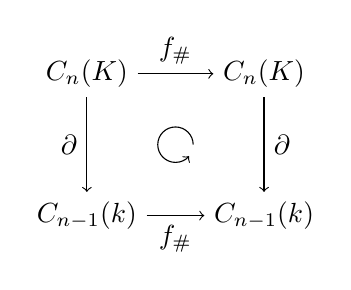
\begin{tikzpicture}[scale=.9]
      \node (00) at (0,0) {$\msf C_n(K)$};
      \node (10) at (2.5,0) {$\msf C_{n}(K)$};
      \node (01) at (0,-2) {$\msf C_{n-1}(k)$};
      \node (11) at (2.5,-2) {$\msf C_{n-1}(k)$};
      \draw[->] (00) -- node[above] {$f_\#$} (10);
      \draw[->] (01) -- node[below] {$f_\#$} (11);
      \draw[->] (00) -- node[left] {$\partial$} (01);
      \draw[->] (10) -- node[right] {$\partial$} (11);
      \draw[->] (1.5, -1) arc (0:320:.25cm);
    \end{tikzpicture}
    \caption{Commutative diagram}
  \end{figure}
\end{problem}
\begin{solution}
  Let $c \in \msf C_n(K)$. Express $c$ as a sum of basis elements
  $\set{\sigma}_{i \in I}$. Let $\set{\sigma_i}_{i \in I'}$ be those $\sigma_i$
  for which $f_{\#}(\sigma_i) \neq \mb 0$. Then
  \begin{align*}
    \partial_{n} (f_{\# n}(c))
    &= \partial_n \pn{\sum_{i\in I'} f_{\# n}(\sigma_i)} \\
    &= \partial_n \pn{\sum_{i \in I'} f(\sigma_i)} \\
    &= \partial_n \pn{\sum_{i\in I'} \set{f\pn{v_0^{(i)}}\cdots f\pn{v_n^{(i)}}}} \\
    &= \sum_{i\in I'} \sum_{j=1}^n \set{f\pn{v_0^{(i)}}\cdots \widehat{f\pn{v_j^{(i)}}}\cdots f\pn{v_n^{(i)}}} \\
    &= \sum_{i \in I'} \sum_{j=1}^n f_{\# n-1} \pn{\simpdel[v^{(i)}]{j}{n}} \\
    &= \sum_{i \in I'} f_{\# n-1}\pn{\partial \pn{\sigma_i}} \\
    &= f_{\# n-1} \pn{ \partial_n \pn{ \sum_{i \in I'} \sigma_i }} \\
    &= f_{\# n-1} \pn{ \partial_n \pn c} \\
  \end{align*}
  as desired.
\end{solution}
\begin{definition}[Induced Homomorphism]
  Let $f : K \to L$ be a simplicial map. The \emph{induced homomorphism} $f_* :
  \msf H_n(K) \to \msf H_n(L)$ is defined by $f_*([z]) = [f_\#(z)]$ (where the
  square brackets indicate an equivalence class).
\end{definition}
\begin{problem}[16.17]
  Let $f : K \to L$ be a simplicial map. Then the induced homomorphism $f_* :
  \msf H_n(K) \to \msf H_n(L)$ is a well-defined homomorphism.
\end{problem}
\begin{solution}
  That $f_*$ is a homomorphism follows directly from the definition.
  \begin{enumerate}[label=(\arabic*)]
  \item That $f_*([\mb 0]) = [\mb 0]$ follows by the definition of $f_{\#}$.
  \item Similarly for $f_*(\sigma + \tau) = f_*(\sigma) + f_*(\tau)$.
  \end{enumerate}
  We now show that $f_*$ is well-defined. Let $[\sigma] \in \msf H_n(K)$ and
  $[\tau] \in \msf H_n(K)$ with $[\sigma] = [\tau]$. Then $\exists \rho \in \msf
  B_n(K) \st \sigma = \tau + \rho$. Observe that
  \begin{align*}
    f_*([\sigma])
    &= [f_{\#}(\sigma)] \\
    &= [f_{\#}(\tau + \rho)] \\
    &= [f_{\#}(\tau) + f_{\#}(\rho)] \\
    &= [f_{\#}(\tau)] + [f_{\#}(\rho)] \\
    &= [f_{\#}(\tau)] + [\mb 0] \\
    &= [f_{\#}(\tau)],
  \end{align*}
  as desired.
\end{solution}
\begin{problem}[16.18]
  Let $K$ be a complex comprising the proper faces of a hexagon: six edges and
  six vertices $v_0, \ldots, v_5$. Let $L$ be the complex comprising the proper
  faces of a triangle: three edges and three vertices $w_0, w_1, w_2$. Let $f$
  be a simplicial map that sends $v_i$ to $w_{i \bmod 3}$. Compute the homology
  groups of $K$ and $L$ and describe the simplicial map $f$ and the induced
  homomorphism $f_*$.
\end{problem}
\begin{solution}
  \begin{enumerate}[label=(\arabic*)]
  \item We compute the homology groups of $K$. Observe, $\msf H_2(K) \cong
    \set{\mb 0}$ (since $\msf Z_n(K)$ is trivial). $\msf H_1(K) \cong
    \zmod{2}$ (since $\msf Z_1(K) \cong \zmod{2}$, as we either have the whole
    hexagon or we don't, and $\msf B_1(K) \cong \set{\mb 0}$). Finally, by
    theorem 16.8, we have $\msf H_0(K) \cong \zmod{2}$.
  \item The homology groups of $L$ are the same.
  \item The map $f$ folds the circle $\abs{K}$ onto itself
  \item $f_*$ is an isomorphism.
  \end{enumerate}
\end{solution}
\begin{definition}[$\lambda$-map]
  Let $K$ be a simplicial complex. Let $\lambda : \sd K \to K$ be defined as
  follows: for any vertex $v \in \sd K$, there exists $\sigma \in K$ such that
  $v$ is the barycenter of $\sigma$. Then let
  \[
    \lambda(v) = v_\sigma
  \]
  where $v_\sigma$ is a vertex in $\sigma$.
\end{definition}
\begin{definition}[$\lambda_*$]
  Let $\lambda_* : \msf H_n(\sd K) \to \msf H_n(K)$ be defined by linear
  extension of $\lambda$ to simplices. Since $\lambda$ is a well-defined
  simplicial map, $\lambda_*$ is a well-defined homomorphism (theorem 16.17).
\end{definition}
\begin{problem}[16.19]
  Suggest a homomorphism from $\msf C_n(K) \to \msf C_n(\sd K)$ that commutes
  with $\partial$. Could its induced homomorphism on homology be an inverse for
  $\lambda_*$?
\end{problem}
\begin{solution}
  Consdier $f : \msf C_n(K) \to \msf C_n(\sd K)$ defined by
  \[
    f(\sigma) = \text{sum of maximal $n$-simplices in $\sd \sigma$}
  \]
\end{solution}
We give this a name.
\begin{definition}[Subdivision operator]
  Define the \emph{subdivision operator} $\SD : \msf C_n(K) \to \msf C_n(\sd K)$
  by first defining $\SD$ on a simplex:
  \[
    \SD(\simp{n}) = \sum_{\mathclap{\pi \in \mc S_{n+1}}} \simp[b^{\pi}]{n}
  \]
  where $\mc S_{n+1}$ is the symmetric group, and $b_k^\pi$ is the barycenter of
  the face $\set{v_{\pi(0)}\cdots v_{\pi(k)}}$.
\end{definition}
\begin{note}
  I'm pretty sure this gets us all the maximal simplices, as we want. To verify
  it, I think we proceed as follows: let $\sigma \in \sd K$ be an arbitrary
  $n$-simplex. Then one of the vertices in $\sigma$ is a vertex in $K$ (def.\ of
  maximal simplex). Take $\pi$ such that $v_{\pi(0)}$ is this maximal vertex.
  Also restrict $\pi$ such that $v_{\pi(1)}$ is the vertex such that the
  barycenter of $\set{v_{\pi(0)}v_{\pi(1)}}$ is in $\sigma$ (again, since
  $\sigma$ is maximal, I think this works). Continue this.

  I think also that one can show this necessitates the resulting simplices be
  disjoint?
\end{note}
\begin{problem}[16.20]
  The subdivision operator commutes with the boundary operator, that is, if $c $
  is a chain in $K$, then $\SD(\partial c) = \partial \SD(c)$.
\end{problem}
\begin{solution}
  We show the result for a simplex. For intuition, observe the following
  diagram in the case $c$ is a $2$-simplex:
  \begin{figure}[H]
    \centering
    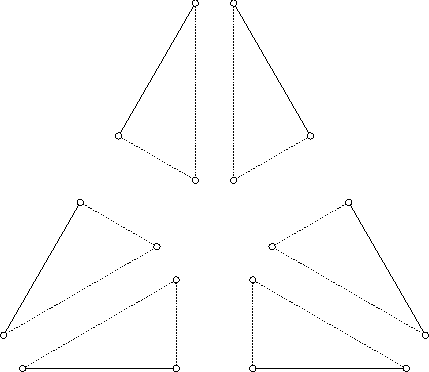
\includegraphics{figures/offset-barycentric-1.pdf}
    \caption{$\SD(c)$}
  \end{figure}
  under $\partial$, only the solid lines are not annihilated. In generality,
  \begin{align*}
    \partial \SD(c)
    &= \partial\sum_{\mathclap{\pi \in \mc S_{n+1}}} \simp[b^\pi]{n} \\
    &= \sum_{\pi \in \mc S_{n+1}} \sum_{j=0}^n \simpdel[b^\pi]{j}{n} \\
    &= \sum_{j=0}^n \sum_{\pi \in \mc S_{n+1}} \simpdel[b^\pi]{j}{n} \\
    &= \sum_{j=0}^{n-1} \sum_{\pi' \in \mc S_{n}} \simp[b^{\pi'}]{n-1} \\
    &= \SD(\partial c)
  \end{align*}
  as desired.\footnote{$\pi'$ is the permutation given by $\pi^{-1}(j_0) =
    \pi(j_0)$, where $j_0$ is the deleted vertex.}
\end{solution}
% \begin{problem}[16.21]
%   Show that $\lambda_\# \circ \SD = \msf{id}$, the identity map on $\msf
%   C_n(K)$, and therefore $\lambda_* \circ \SD_* = \msf{id}_*$, the identity map
%   on $\msf H_n(K)$.
% \end{problem}
% \begin{solution}
%   Recall the definition:
%   \[
%     \lambda_\# \sigma_i
%     =
%     \begin{cases}
%       \mb 0 & \text{if } f(\sigma_i) \text{ is not an $n$-simplex}, \\
%       \lambda(\sigma) & \text{otherwise.}
%     \end{cases}
%   \]
% \end{solution}

\begin{note}
  \color{green} I think that it's getting a little tricky here to see which
  concepts are the ``important parts.'' Maybe let's shift to trying
  \texttt{http://www.indiana.edu/~lniat/m621notessecondedition.pdf}
\end{note}

\section{The Mayer-Vietoris Theorem}
\begin{definition}[Subcomplex]
  If $K$ is a simplicial complex, a \emph{subcomplex} is a simplicial complex
  $L$ such that $L \subset K$.
\end{definition}
\begin{note}
  The thing to note here is that if we choose some simplex to be in our
  subcomplex, we must bring all its faces with us as well.
\end{note}
\begin{problem}[16.31]
  If $K$ is a finite simplicial complex, verify that the intersection of two
  subcomplexes of $K$ is a subcomplex.
\end{problem}
\begin{solution}
  Let $L, M$ be subcomplexes of $K$. Then for all $\sigma \in L \cap
  M$, $\sigma \in L,\ \sigma \in M$, hence for all faces $\sigma'
  \subset \sigma$, we have $\sigma' \in L,\ \sigma' \in M$, and thus
  $\sigma'\in L \cap M$. Hence $L \cap M$ is a simplicial complex.

  The disjointness condition follows similarly.
\end{solution}

We'll now examine cases where we have two subcomplexes $A,B$ of a
simplicial complex $K$. We want to look at relationships between
cycles in $A,B, A\cap B$, and $K$.

\begin{figure}[H]
  \centering
  \begin{subfigure}{.4\linewidth}
    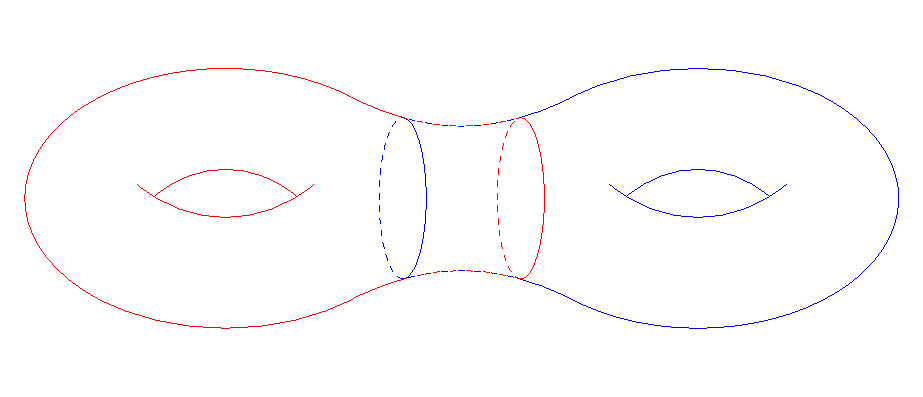
\includegraphics[width=\linewidth, keepaspectratio]{figures/mayer-vie-torus}
  \end{subfigure}
  \begin{subfigure}{.18\linewidth}
    \begin{tikzpicture}
      \draw[->] (-1,1) -- (1,1);
    \end{tikzpicture}
  \end{subfigure}
  \begin{subfigure}{.4\linewidth}
    \hspace{-.8cm}
    ~\vspace{-.5cm}
    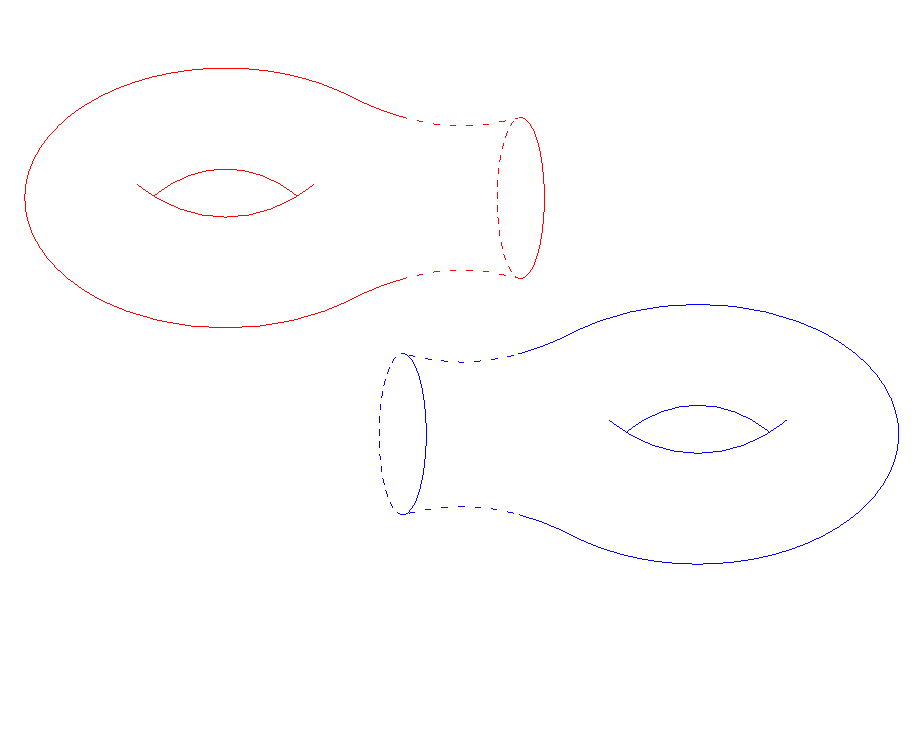
\includegraphics[width=\linewidth, keepaspectratio]{figures/mayer-vie-torus-sep}
  \end{subfigure}
  \caption{An example of such $A,B$}
\end{figure}

\begin{problem}[16.32]
  Note that a cycle in $A \cap B$ is still a cycle in $A$, $B$, and
  $K$. Then answer:
  \begin{enumerate}
  \item Can a trivial cycle in $A \cap B$ be non-trivial in $A$?
  \item Can a non-trivial cycle in $A \cap B$ be trivial in $A$?
  \item Can a non-trivial cycle in $A \cap B$ that's also
    non-trivial in $A$ and in $B$ be trivial in $K$?
  \end{enumerate}
\end{problem}
\begin{solution}
  Let $\sigma \in A \cap B$. I'll assume this is asking us to just
  consider just the inclusion map applied to $\sigma$
  \begin{enumerate}
  \item Nope. Including into $A$ won't change $\sigma$ at all.
  \item No?
  \item No?
  \end{enumerate}
\end{solution}

\begin{definition}[``Intersection'' map]
  Let $A,B$ be subcomplexes of a simplicial complex $K$. Define the
  homomorphisms $\pi_A : \msf Z_k(K) \to \msf Z_k(A)$, $\pi_B : \msf
  Z_k(K) \to \msf Z_k(B)$ as follows:
  \[
    \pi_A(\sigma) =
    \begin{cases}
      \sigma & \text{if } \sigma \in \msf Z_k(A) \\
      \mb 0 & \text{otherwise}
    \end{cases}
    \qquad\qquad
    \pi_B(\sigma) =
    \begin{cases}
      \sigma & \text{if } \sigma \in \msf Z_k(B) \\
      \mb 0 & \text{otherwise}
    \end{cases}
  \]
  Observe that the following diagram commutes, and that $\pi_A$,
  $\pi_B$ are idempotent:\footnote{Ok, technically $\dom \pi_A = \msf
    Z_k(K) \neq \msf Z_k(B)$, but you could throw an inclusion map in
    there if you so pleased.}
  \begin{figure}[H]
    \centering
    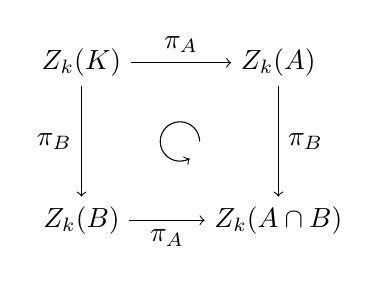
\begin{tikzpicture}
      \node (K) at (-1.25,1) {$\msf Z_k(K)$};
      \node (A) at (1.25,1) {$\msf Z_k(A)$};
      \node (B) at (-1.25,-1) {$\msf Z_k(B)$};
      \node (AcB) at (1.25,-1) {$\msf Z_k(A\cap B)$};

      \draw[->] (K) -- (A) node[midway, above] {$\pi_A$};
      \draw[->] (A) -- (AcB) node[midway, right] {$\pi_B$};
      \draw[->] (K) -- (B) node[midway, left] {$\pi_B$};
      \draw[->] (B) -- (AcB) node[midway, below] {$\pi_A$};

      \pgfmathsetmacro{\r}{.25}
      \draw[->] (\r,0) arc(0:300:\r);
    \end{tikzpicture}
    \caption{$\pi_A \circ \pi_B = \pi_B \circ \pi_A$}
  \end{figure}
\end{definition}

\begin{problem}[16.33]
  Let $K$ be a finite simplicial complex and $A$ and $B$ be
  subcomplexes such that $K=A\cup B$. If $\alpha$, $\beta$ are
  $k$-cycles in $A$ and $B$ respectively, and if $\alpha
  \sim_{\zmod{2}} \beta$ in $K$, then there is a $k$-cycle $c$ in
  $A\cap B$ such that $\alpha \sim_{\zmod{2}} c$ in $A$ and $\beta
  \sim_{\zmod{2}} c$ in $B$.
\end{problem}
\begin{solution}
  The question can be rephrased as
  \begin{leftbar}
    Let $\alpha \in \msf Z_k(A)$, and $\beta \in \msf Z_k(B)$. Suppose
    that
    \[
      [\alpha]_K = [\beta]_K.
    \]
    Then there exists $c \in \msf Z_k(A \cap B)$ such that
    \[
      [\alpha]_A = [c]_A \qquad\qquad [\beta]_B = [c]_B
    \]

    Or, show that if $\alpha - \beta = 0 \in \msf H_k(K)$, then
    $\exists c \in \msf Z_k(A \cap B)$ such that $(\alpha, \beta) =
    (c,c) \in \msf H_k(A) \oplus \msf H_k(B)$. This gives us maps
    \[
      \msf H_n(K) \xrightarrow{\delta^{k}} \msf H_k(A \cap B)
      \xrightarrow{\phi^{k}}  \msf H_k(A) \oplus \msf H_k(B)
    \]
    by
    \[
      [\alpha] = [\beta] \xmapsto{\delta^k} [c] \xmapsto{\phi^k}
      [(c,c)]
    \]
  \end{leftbar}
  Since $[\alpha]_K = [\beta]_K$, there exists $c_0 \in \msf B_k(K)$
  such that $\alpha - \beta = c_0$. By definition of $\msf B_n(K)$,
  this implies that there exists $\gamma \in \msf C_{k+1}(K)$ with
  $c_0 = \partial \gamma$.

  \textbf{Claim:} $c = \alpha + \partial \pi_A(\gamma)$ works.

  \textbf{Proof of Claim:}
  \begin{enumerate}
    \item First, we show $c$ is a $k$-cycle. Note
      \begin{align*}
        \partial c
        &= \partial \alpha + \partial^2 \pi_A(\gamma) \\
        &= \partial \alpha = \mb 0
      \end{align*}
      as desired.
    \item Now, we verify that equivalences. First, note that $c-\alpha
      = \partial \pi_A(\gamma)$, hence $[\alpha]_A = [c]_A$ trivially.
      Now,
      \begin{align*}
        c-\beta
        &= c - \alpha + \alpha - \beta & (0=\alpha - \alpha)\\
        &= (c-\alpha) + \alpha - \beta & (\text{grouping})\\
        &= \partial \pi_A(\gamma) + \alpha - \beta & (c-\alpha=\partial \pi_A(\gamma))\\
        &= \partial \pi_A(\gamma) + c_0 & (c_0 = \alpha - \beta)\\
        &= \partial \pi_A(\gamma) + \partial \gamma & (\partial \gamma = c_0)\\
        &= \partial (\pi_A\gamma + \gamma) & (\partial \text{ commutes})
      \end{align*}
      hence $c - \beta \in \msf B_k(K)$. So $[c]_B = [\beta]_B$, as
      desired.
  \end{enumerate}
\end{solution}

\begin{problem}[16.34]
  Let $K$ be a finite simplicial complex and $A$ and $B$ be
  subcomplexes such that  $K=A\cup B$. Let $z$ be a $k$-cycle in $K$.
  Then there exist $k$-chains $\alpha$ and $\beta$ in $A$ and $B$
  respectively such that:
  \begin{enumerate}[label=(\arabic*)]
    \item $z=\alpha+\beta$ and
    \item $\partial \alpha=\partial \beta$ is a $(n-1)$-cycle $c$ in
      $A\cap B$.
    \item If $z= \alpha'+\beta'$, a sum of $n$-chains in $A$ and $B$
      respectively, and $c'= \partial \alpha' = \partial \beta'$ is a
      $(n-1)$-cycle, then $c'$ is homologous to $c$ in $A \cap B$.
  \end{enumerate}
\end{problem}

\begin{solution}
  \begin{enumerate}[label=(\arabic*)]
    \item Let $\alpha = \pi_A(z)$. Then $\alpha \in \msf C_k(A)$. Now,
      taking $\beta = z - \alpha$, we see
      \begin{align*}
        \pi_A(\beta)
        &= \pi_A(z - \alpha) \\
        &= \pi_A(z - \pi_A(\alpha)) \\
        &= \pi_A(z) - \pi_A(\pi_A(z)) \\
        &= \pi_A(z) - \pi_A(z) \\
        &= \mb 0
      \end{align*}
      hence $\beta \in \msf C_k(B)$.
    \item WTS $\partial \alpha = \partial \beta \in \msf Z_{n-1}(A
      \cap B)$. Note,
      \begin{align*}
        \partial(\beta)
        &= \partial(z - \alpha) \\
        &= \partial(z) - \partial(\alpha) \\
        &= \mb 0 -\partial(\alpha) = \partial(\alpha),
      \end{align*}
      which are $(n-1)$-boundaries (and hence $(n-1)$-cycles).
      Projection onto $A \cap B$ yields the desired result.
    \item In $A \cap B$, $c$ and $c'$ are both $(n-1)$ boundaries.
      Hence, they are trivially homologous.
  \end{enumerate}
\end{solution}

\begin{problem}[16.36]
  Let $K$ be a simplicial complex and $A$ and $B$ be subcomplexes such
  that $K=A\cup B$. Construct natural homomorphisms $\phi,\psi,\delta$
  among the groups below and show that $\psi \circ \phi =0$ and
  $\delta \circ \psi = 0$.
  \begin{enumerate}
    \item $\phi: \msf H_n(A\cap B)\to \msf H_n(A)\oplus \msf H_n(B)$.
    \item $\psi: \msf H_n(A)\oplus \msf H_n(B)\to \msf H_n(K)$.
    \item $\delta: \msf H_n(K)\to \msf H_{n-1}(A\cap B)$.
  \end{enumerate}
\end{problem}
\begin{solution}
  Let
  \begin{enumerate}[label=(\arabic*)]
    \item $\phi : \msf H_n(A \cap B) \to \msf H_n(A) \oplus \msf
      H_n(B)$ be given by
      \[
        \phi(\sigma) = (\sigma, \sigma).
      \]
      That this is a well-defined homomorphism follows immediately.
    \item Let $\psi(\sigma, \tau)$ be given by
      \[
        \psi(\alpha,\beta) = \alpha - \beta.
      \]
      It is straightforward to verify this is a well-defined
      homomorphism.
    \item Let $\sigma \in \msf H_n(K)$, and take $\tau \in \msf
      Z_n(K)$ a representative of $\sigma$. Then $\exists c \in \msf
      B_n(K)$ such that
      \[
        \sigma + \tau = c.
      \]
      Then by the theorem above, there exists $\alpha \in \msf C_n(A),
      \beta \in \msf C_n(B)$
      such that
      \[
        \alpha + \beta = c.
      \]
      Further, $\partial \alpha$, $\partial \beta$ is an $(n-1)$-cycle
      $c'$ in $A \cap B$.

      Let $\delta(\sigma)$ be given by
      \[
        \delta(\sigma) = \partial(\pi_A \sigma).
      \]
      That this is a well-defined homomorphism follows, since all the
      maps included are linear.
  \end{enumerate}
  Now, we show the composition things.
  \begin{enumerate}
    \item
      \begin{align*}
        \psi \circ \phi(\alpha)
        &= \psi(\alpha, \alpha) \\
        &= \alpha - \alpha \\
        &= \mb 0
      \end{align*}
      as desired.
    \item Let $\alpha \in \msf H_n(A)$, $\beta \in \msf H_n(B)$. Then
      by the theorem above, there exists
      \begin{align*}
        \delta(\psi(\alpha, \beta))
        &= \partial (\pi_A (\alpha - \beta)) \\
        &= \partial(\alpha - \pi_A(\beta))
      \end{align*}
      \begin{figure}[H]
        \centering
        \includegraphics[width=\linewidth, keepaspectratio]{figures/two-torus-AB}
        \caption{Example of $A,B$ with $\alpha, \beta$.}
      \end{figure}
  \end{enumerate}
\end{solution}


\begin{definition}[Exact sequence]
  Given a (finite or infinite) sequence of groups and homomorphisms:
  \[
    \cdots \to G_{i-1}\stackrel{\phi_{i-1}}{\longrightarrow} G_{i}
    \stackrel{\phi_i}{\longrightarrow}G_{i+1} \to \cdots
  \]
  the sequence is \textbf{exact at $G_i$} if and only if $\im
  \phi_{i-1}=\ker \phi_{i}$. The sequence is called an \textbf{exact
    sequence} if and only if it is exact at each group (except at the
  first and last groups if they exist).
\end{definition}


\begin{problem}[16.37]
  Let $K$ be a finite simplicial complex and $A$ and $B$ be
  subcomplexes such that $K=A\cup B$. The sequence
  \[
    \dots \to \msf H_n(A\cap B) \to \msf H_n(A)\oplus \msf H_n(B) \to
    \msf H_n(K) \to \msf H_{n-1}(A\cap B) \to \dots
  \]
  using the homomorphisms $\phi,\psi,\delta$ above, is exact.
\end{problem}

\begin{enumerate}
  \item
\end{enumerate}

\begin{problem}[16.39]
  Compute the $\zmod 2$-homology groups for each complex $K$ below.
  \begin{enumerate}
    \item The bouquet of $k$ circles (the union of $k$ circles
      identified at a point).
    \item A wedge of a $2$-sphere and a circle (the two spaces are
      glued at one point).
    \item A $2$-sphere union its equatorial disk.
    \item A double solid torus.
  \end{enumerate}
\end{problem}
\begin{solution}
  \begin{enumerate}
    \item $K$ is given by $k$ triangles (together with their faces),
      with one common vertex. Hence
      \[
        \msf H_1(K) = (\zmod{2})^k \qquad\qquad \msf H_0(K) =
        (\zmod{2})^k
      \]
    \item Observe that $K = \partial \Delta^3 \cup \partial \Delta^2 /
      v_1 \sim v_2$ (where $v_1$, $v_2$ are arbitrarily chosen
      vertices from $\partial \Delta^3$, $\partial \Delta^2$
      respectively). There are just two elements of $\msf H_2(K)$:
      namely, $\mb 0$ and $A_1 + A_2 + A_3 + A_4$. Hence, $\msf H_2(K)
      \cong \zmod{2}$.

      Now, since $\partial^2 \Delta^3 = 0$, $\msf H_1(\partial^2
      \Delta^3)$ is trivial. Observe that $\msf H_1(\partial \Delta^2)
      = \zmod{2}$. Now,
    \item
    \item
  \end{enumerate}
\end{solution}


\begin{problem}[16.40]
  Compute the $\zmod{2}$-homology groups of a torus using
  Mayer-Vietoris in two different ways (with two different
  decompositions).
\end{problem}
\begin{solution}
  By Mayer-Vietoris, independent of our particular decomposition, we
  will have the following exact sequence:
  \begin{figure}[H]
    \centering
    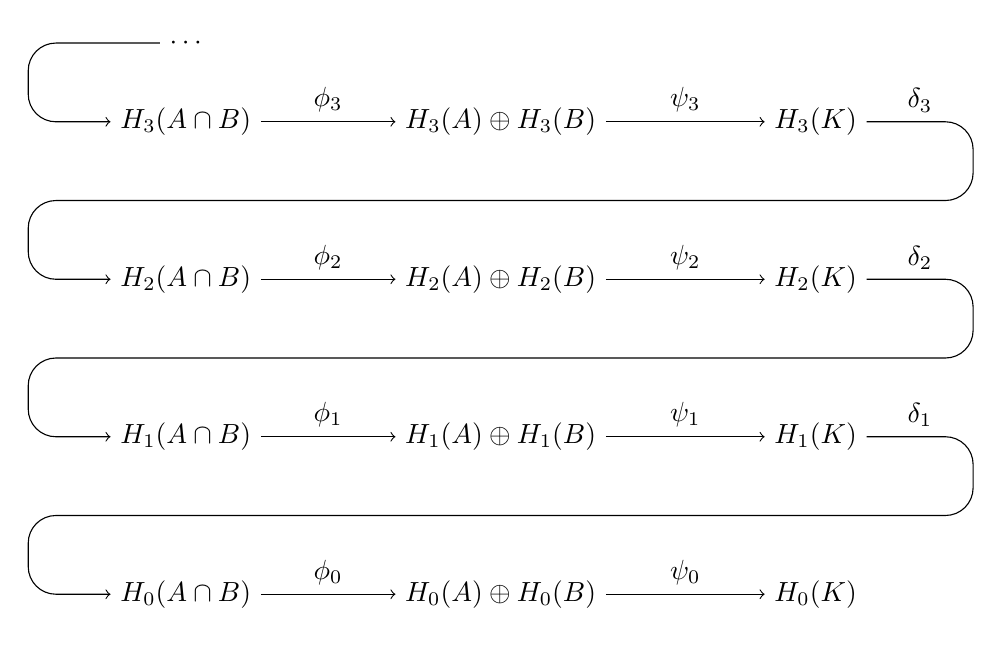
\begin{tikzpicture}
      \pgfmathsetmacro{\xmin}{-6};
      \pgfmathsetmacro{\xmax}{6};
      \pgfmathsetmacro{\ymin}{-3};
      \pgfmathsetmacro{\ymax}{3};
      % \draw[help lines, color=gray!30, dashed] (\xmin,\ymin) grid (\xmax,\ymax);
      % \draw[->] (\xmin,0)--(\xmax,0) node[right]{$x$};
      % \draw[->] (0,\ymin)--(0,\ymax) node[above]{$y$};

      \node (cdots) at (-4,5) {$\cdots$};

      \node (3acb) at (-4, 4) {$\msf H_3(A \cap B)$};
      \node (3apb) at (0,4) {$\msf H_3(A) \oplus \msf H_3(B)$};
      \node (3k) at (4,4) {$\msf H_3(K)$};


      \node (2acb) at (-4,2) {$\msf H_2(A \cap B)$};
      \node (2apb) at (0,2) {$\msf H_2(A) \oplus \msf H_2(B)$};
      \node (2k) at (4,2) {$\msf H_2(K)$};

      \node (1acb) at (-4,0) {$\msf H_1(A \cap B)$};
      \node (1apb) at (0,0) {$\msf H_1(A) \oplus \msf H_1(B)$};
      \node (1k) at (4,0) {$\msf H_1(K)$};

      \node (0acb) at (-4,-2) {$\msf H_0(A \cap B)$};
      \node (0apb) at (0,-2) {$\msf H_0(A) \oplus \msf H_0(B)$};
      \node (0k) at (4,-2) {$\msf H_0(K)$};

      \draw[->, rounded corners=10pt] (cdots) -- ($(3acb) + (-2,1)$) -- ++(0,-1) -- (3acb);

      \draw[->] (3acb) -- (3apb) node[midway, above] {$\phi_3$};
      \draw[->] (3apb) -- (3k) node[midway, above] {$\psi_3$};
      \draw[->, rounded corners=10pt] (3k) -- ++(2,0) node[midway, above] {$\delta_3$} -- ++(0,-1) -- ($(2acb) + (-2,1)$) -- ++(0,-1) -- (2acb);

      \draw[->] (2acb) -- (2apb) node[midway, above] {$\phi_2$};
      \draw[->] (2apb) -- (2k) node[midway, above] {$\psi_2$};
      \draw[->, rounded corners=10pt] (2k) -- ++(2,0) node[midway, above] {$\delta_2$} -- ++(0,-1) -- ($(1acb) + (-2,1)$) -- ++(0,-1) -- (1acb);

      \draw[->] (1acb) -- (1apb) node[midway, above] {$\phi_1$};
      \draw[->] (1apb) -- (1k) node[midway, above] {$\psi_1$};
      \draw[->, rounded corners=10pt] (1k) -- ++(2,0) node[midway, above] {$\delta_1$} -- ++(0,-1) -- ($(0acb) + (-2,1)$) -- ++(0,-1) -- (0acb);
      \draw[->] (0acb) -- (0apb) node[midway, above] {$\phi_0$};
      \draw[->] (0apb) -- (0k) node[midway, above] {$\psi_0$};
    \end{tikzpicture}
    \caption{Mayer Vie-torus (heh)}
  \end{figure}
  Let $A,B$ be two macaroni elbow shapes, overlapping on two
  cylindrical segments:
  \begin{figure}[h]
    \centering
    % \includegraphics[keepaspectratio,width=.5\linewidth,angle=270]{figures/mathematica-torus-decomp}
    \caption{Decomposition 1: $\color{green} A$ below, $\color{orange}
      B$ above}
  \end{figure}
  Note that for $k > 2$, $\TT^2$ has no $k$-cycles, and hence
  \[
    \msf H_k(A\cap B)  \cong \msf H_k(A) \oplus \msf H_k(B) \cong \msf
    H_k(\TT^2) = \set{\mb 0}.
  \]
  by exactness of the Mayer-Vietoris sequence, $\im \delta_3 = \ker
  \phi_2 = \set{\mb 0}$. Hence, $\phi_2$ is one-to-one. We will use
  this later.

  Calculating the $n=1,0$ homology groups is easy. By Theorem 16.8,
  $\msf H_0(A \cap B) \cong \zmod{2} \times \zmod{2}$, $\msf H_0(A)
  \oplus \msf H_0(B) \cong \zmod{2}\times \zmod{2}$, and $\msf
  H_0(\TT^2) \cong \zmod{2}$.

  Now, observe that each of $\msf H_2(A \cap B)$, $\msf H_2(A)$, and
  $\msf H_2(B)$ are trivial ($A$ and $B$ bound no volume). Hence
  $\delta_2$ is injective. Furthermore, since $A \cap B$ is a disjoint
  union of two cylinders, $\msf H_1(A \cap B) \cong \zmod{2} \times
  \zmod{2}$, and $\msf H_1(A) \cong \msf H_1(B) \cong \zmod{2}$. This
  gives
  \begin{figure}[H]
    \centering
    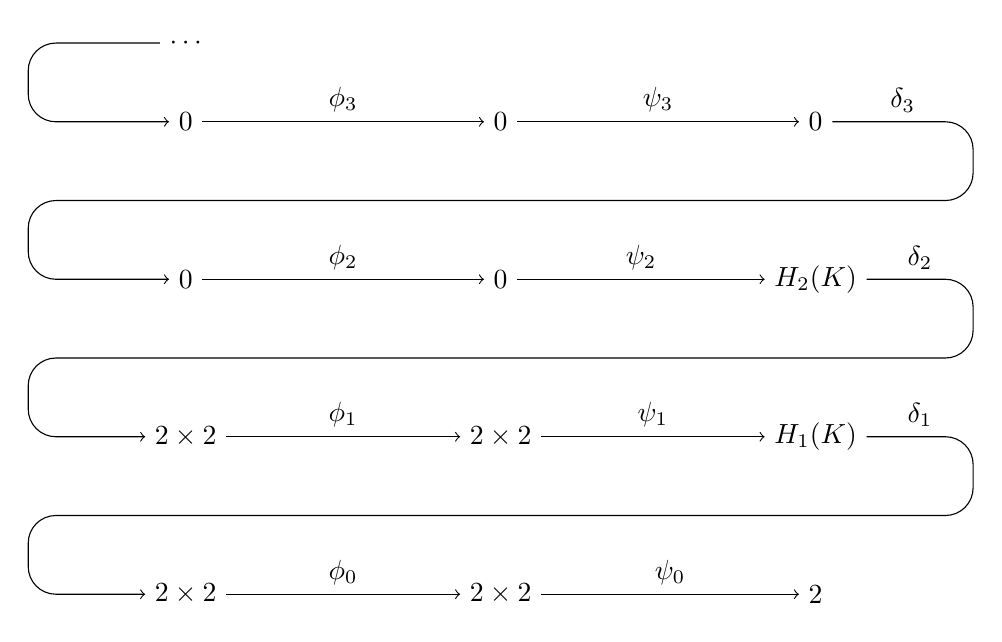
\begin{tikzpicture}
      \pgfmathsetmacro{\xmin}{-6};
      \pgfmathsetmacro{\xmax}{6};
      \pgfmathsetmacro{\ymin}{-3};
      \pgfmathsetmacro{\ymax}{3};

      \node (cdots) at (-4,5) {$\cdots$};

      \node (3acb) at (-4, 4) {$\set{\mb 0}$};
      \node (3apb) at (0,4) {$\set{\mb 0}$};
      \node (3k) at (4,4) {$\set{\mb 0}$};


      \node (2acb) at (-4,2) {$\set{\mb 0}$};
      \node (2apb) at (0,2) {$\set{\mb 0}$};
      \node (2k) at (4,2) {$\msf H_2(K)$};

      \node (1acb) at (-4,0) {$\zmod{2} \times \zmod{2}$};
      \node (1apb) at (0,0) {$\zmod{2} \times \zmod{2}$};
      \node (1k) at (4,0) {$\msf H_1(K)$};

      \node (0acb) at (-4,-2) {$\zmod{2} \times \zmod{2}$};
      \node (0apb) at (0,-2) {$\zmod{2} \times \zmod{2}$};
      \node (0k) at (4,-2) {$\zmod{2}$};

      \draw[->, rounded corners=10pt] (cdots) -- ($(3acb) + (-2,1)$) -- ++(0,-1) -- (3acb);

      \draw[->] (3acb) -- (3apb) node[midway, above] {$\phi_3$};
      \draw[->] (3apb) -- (3k) node[midway, above] {$\psi_3$};
      \draw[->, rounded corners=10pt] (3k) -- ++(2,0) node[midway, above] {$\delta_3$} -- ++(0,-1) -- ($(2acb) + (-2,1)$) -- ++(0,-1) -- (2acb);

      \draw[->] (2acb) -- (2apb) node[midway, above] {$\phi_2$};
      \draw[->] (2apb) -- (2k) node[midway, above] {$\psi_2$};
      \draw[->, rounded corners=10pt] (2k) -- ++(2,0) node[midway, above] {$\delta_2$} -- ++(0,-1) -- ($(1acb) + (-2,1)$) -- ++(0,-1) -- (1acb);

      \draw[->] (1acb) -- (1apb) node[midway, above] {$\phi_1$};
      \draw[->] (1apb) -- (1k) node[midway, above] {$\psi_1$};
      \draw[->, rounded corners=10pt] (1k) -- ++(2,0) node[midway, above] {$\delta_1$} -- ++(0,-1) -- ($(0acb) + (-2,1)$) -- ++(0,-1) -- (0acb);
      \draw[->] (0acb) -- (0apb) node[midway, above] {$\phi_0$};
      \draw[->] (0apb) -- (0k) node[midway, above] {$\psi_0$};
    \end{tikzpicture}
    \caption{Summary of results so far}
  \end{figure}
  Finally, we apply exactness. Since $\dom{\psi_2} = \set{\mb 0}$,
  $\im \psi_2 = \ker \delta_2 = \set{\mb 0}$, hence $\delta_2$ is 1-1.
  Now, note that $\ker \psi_1 = \set{(0,0), (1,1)} = \im \phi_1$.
  Hence, $\ker \phi_1 \cong \zmod{2} \cong \im \delta_2$. It follows
  that $\msf H_2(K) \cong \zmod{2}$.
  \begin{figure}[H]
    \centering
    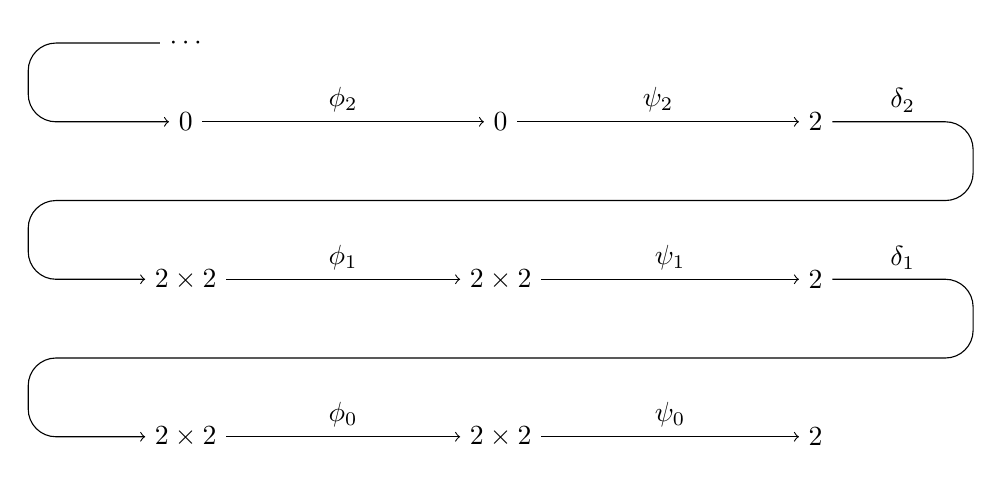
\begin{tikzpicture}
      \pgfmathsetmacro{\xmin}{-6};
      \pgfmathsetmacro{\xmax}{6};
      \pgfmathsetmacro{\ymin}{-3};
      \pgfmathsetmacro{\ymax}{3};

      \node (cdots) at (-4,3) {$\cdots$};

      \node (2acb) at (-4,2) {$\set{\mb 0}$};
      \node (2apb) at (0,2) {$\set{\mb 0}$};
      \node (2k) at (4,2) {$\zmod{2}$};

      \node (1acb) at (-4,0) {$\zmod{2} \times \zmod{2}$};
      \node (1apb) at (0,0) {$\zmod{2} \times \zmod{2}$};
      \node (1k) at (4,0) {$\zmod{2}$};

      \node (0acb) at (-4,-2) {$\zmod{2} \times \zmod{2}$};
      \node (0apb) at (0,-2) {$\zmod{2} \times \zmod{2}$};
      \node (0k) at (4,-2) {$\zmod{2}$};

      \draw[->, rounded corners=10pt] (cdots) -- ($(2acb) + (-2,1)$) -- ++(0,-1) -- (2acb);

      \draw[->] (2acb) -- (2apb) node[midway, above] {$\phi_2$};
      \draw[->] (2apb) -- (2k) node[midway, above] {$\psi_2$};
      \draw[->, rounded corners=10pt] (2k) -- ++(2,0) node[midway, above] {$\delta_2$} -- ++(0,-1) -- ($(1acb) + (-2,1)$) -- ++(0,-1) -- (1acb);

      \draw[->] (1acb) -- (1apb) node[midway, above] {$\phi_1$};
      \draw[->] (1apb) -- (1k) node[midway, above] {$\psi_1$};
      \draw[->, rounded corners=10pt] (1k) -- ++(2,0) node[midway, above] {$\delta_1$} -- ++(0,-1) -- ($(0acb) + (-2,1)$) -- ++(0,-1) -- (0acb);
      \draw[->] (0acb) -- (0apb) node[midway, above] {$\phi_0$};
      \draw[->] (0apb) -- (0k) node[midway, above] {$\psi_0$};
    \end{tikzpicture}
    \caption{Final diagram}
  \end{figure}
  we now take the second decomposition.
  \begin{figure}[h]
    \centering
    % \includegraphics[width=.5\linewidth, keepaspectratio]{figures/mathematica-torus-decomp-2}
    \caption{Second Decomposition}
  \end{figure}
  For $k > 2$, all the results remain the same. Now, note that $A \cap
  B$ is given by two concentric cylinders. Since this is still the
  disjoint union of two cylinders, for $k = 0,1,2$ the homology groups
  $H_k(A \cap B)$ and $H_k(A) \oplus H_k(B)$ remain the same. Thus, an
  identical argument to that above shows that $\msf H_2(\TT^2)$, $\msf
  H_1(\TT^2)$ are likewise identical.
\end{solution}

\begin{problem}[FS1]
  Suppose that $K$ is a triangulation of two copies of $\sS^2$,
  identified at a copy of $\sS^1$. Let $A \cong \sS^2 \cong B$. Use
  Mayer-Vietoris to compute $\msf H_n(K)$.
\end{problem}
\begin{solution}
  As before, all the $\msf H_k$ are trivial for $k > 2$. For $k=0$, we
  count the number of connected components. This yields
  \begin{itemize}
    \item $\msf H_0(K) \cong \zmod{2}$
    \item $\msf H_0(A) \oplus \msf H_0(B) \cong (\zmod{2})^2$
    \item $\msf H_0(A \cap B) \cong \zmod{2}$
  \end{itemize}
  For $k=1$,
  \begin{itemize}
    \item $\msf H_1(A\cap B) \cong \zmod{2}$
    \item $\msf H_1(A) \oplus \msf H_1(B) \cong (\zmod{2})^2$
    \item
  \end{itemize}
\end{solution}

\begin{problem}[16.41]
  Use the Mayer-Vietoris Theorem to compute $\msf H_n(M)$ for every
  compact, triangulated $2$-manifold $M$. What compact, triangulated
  $2$-manifolds are not distinguished from one another by
  $\zmod{2}$-homology? What does $\msf H_2(M)$ tell you?
\end{problem}
\begin{solution}
  Let $M$ be a compact triangulated 2-manifold, and call the
  triangulation $K$. Let $A,B$ be subcomplexes of $K$ such that $A
  \cup B = K$. Then for all $k > 2$, each of $\msf H_k(M)$, $\msf
  H_k(A)$, $\msf H_k(B)$, and $\msf H_k(A) \oplus \msf H_k(B)$ are
  isomorphic to $\set{\mb 0}$.

  Suppose $M$ can be expressed as the following connected sum:
\end{solution}


\begin{problem}[16.42]
  Let $p,q\in\ZZ$ be relatively prime. Calculate $\msf H_n(L(p,q))$,
  the homology of the lens space $L(p,q)$.
\end{problem}



%%% Local Variables:
%%% TeX-master: "../main"
%%% TeX-engine: default-shell-escape
%%% TeX-command-extra-option: -pdf
%%% End:

\chapter[$\ZZ$ Homology]{Simplicial $\ZZ$-Homology: Getting Oriented}
\section{Orientation and $\ZZ$-Homology}
\begin{note}
  We used $\msf H_n(K)$ to denote the $\zmod{2}$-homology gorups of a
  complex $K$. This was to simplify notation. In general, the notation
  is more like $\msf H_n(K; G)$, where $G$ is the group of
  coefficients for our module. When $G=\ZZ$, we drop the group and
  write $\msf H_n(K)$.
\end{note}

\begin{definition}[Edge orientation]
  For an edge $\set{vw}$, the two orientation classes correspond to
  two orderings of the vertices $v$ and $w$, and are denoted $\bk{vw}$
  and $\bk{wv}$. It is customary to think of the oriented edge
  $\bk{vw}$ as an edge with an arrow pointing from $v$ to $w$. We set
  $\bk{vw} = -\bk{wv}$.
\end{definition}
\begin{figure}[h]
  \centering
  \begin{tikzpicture}[
    decoration={
      markings,
      mark=at position 0.5 with {\arrow{>}}
    }]
    \node[draw, circle, fill=black, inner sep=1pt] (v1) at (-1,1) {};
    \node[above left] (v1l) at (v1) {$v$};
    \node[draw, circle, fill=black, inner sep=1pt] (w1) at (-1,-1) {};
    \node[below left] (w1l) at (w1) {$w$};
    \draw[thick, postaction={decorate}] (v1) -- (w1);

    \node[draw, circle, fill=black, inner sep=1pt] (v2) at (1,1) {};
    \node[above left] (v2l) at (v2) {$v$};
    \node[draw, circle, fill=black, inner sep=1pt] (w2) at (1,-1) {};
    \node[below left] (w2l) at (w2) {$w$};
    \draw[thick, postaction={decorate}] (w2) -- (v2);
  \end{tikzpicture}
  \caption{$\bk{vw}$ and $\bk{wv}$}
\end{figure}

\begin{definition}[Triangle orientation]
  For a triangle $\set{uvw}$ with vertices $u$, $v$, and $w$, the two
  orientation classes correspond geometrically to clockwise or
  counterclockwise orderings of the vertices when viewed a long a
  fixed normal.
\end{definition}

\begin{definition}[Oriented Simplex]
  Let $\simp{k}$ be a $k$-simplex, and let $\pi \in \mc S_n$. Then
  \[
    [v_0 \cdots v_k] = [v_{\pi(0)} \cdots v_{\pi(k)}]
  \]
  iff $\pi \in A_n$. If $\pi \not\in A_n$, we have
  \[
    [v_0 \cdots v_k] = -[v_{\pi(0)} \cdots v_{\pi(k)}]
  \]
  An $n$-simplex with a chosen orientation is called a \emph{Oriented
    simplex}. The boundary of a $0$-simplex is defined to be $0$.
\end{definition}

\begin{definition}[$n$-chain group]
  The $n$-\emph{chain group of $K$} is the free abelian group of
  oriented $K$-simplices under the equivalence relation above.
\end{definition}

\begin{definition}[Boundary map]
  For $n \geq 1$, the \emph{boundary of an oriented $n$-simplex}
  $\sigma = [v_0 \cdots v_n]$ is
  \[
    \partial(\sigma) = \sum_{i=0}^n (-1)^i \osimpdel{i}{n}
  \]
\end{definition}

\begin{problem}[18.3]
  For any $n$-simplex $\sigma$,
  \[
    \partial(-\sigma) = -\partial(\sigma)
  \]
\end{problem}
\begin{solution}
  Let $\sigma = \osimp{n}$. Since $(0\ 1)$ is odd, then
  \begin{align*}
    \osimp{n} = -\bk{v_1v_0\cdots v_n}
  \end{align*}
  hence
  \begin{align*}
    \partial(-\sigma)
    &= \partial(\bk{v_1v_0\cdots v_n}) \\
    &= \sum_{i=0}^n (-1)^i \osimpdel{i}{n} \\
    &= \bk{v_0v_2\cdots v_n} - \bk{v_1v_2 \cdots v_n} + \bk{v_1v_0v_3\cdots v_n} + \cdots + (-1)^n\bk{v_1v_0\cdots v_{n-1}} \\
    &= -\bk{v_1v_2\cdots v_n} + \bk{v_1v_2 \cdots v_n} - \bk{v_0v_1v_3\cdots v_n} + \cdots + (-1)^{n+1}\bk{v_0v_1\cdots v_{n-1}} \\
    &= \sum_{i=0}^n (-1)^{i+1} \osimpdel{i}{k} \\
    &= -\partial(\sigma)
  \end{align*}
  as desired.
\end{solution}
\begin{definition}[Boundary of an $n$-chain]
  The boundary of an $n$-chain is an $(n-1)$-chain given by
  \[
    \partial\pn{\sum_{i=1}^k c_i \sigma_i}
    = \sum_{i=1}^k c_i\partial(\sigma_i)
  \]
  Thus, the boundary is a homomorphism
  \[
    \partial_n : \msf C_n(K) \to \msf C_{n-1}(K)
  \]
\end{definition}
\begin{problem}[18.4]
  For all $n \geq 0$,
  \[
    \partial_n \circ \partial_{n+1}=0.
  \]
\end{problem}
\begin{solution}
  Let $\sigma \in \msf C_{n+1}(K)$ be given by
  \[
    \sigma = \sum_{i=0}^k c_i \sigma_i.
  \]
  Then
  \begin{align*}
    \partial_n \circ \partial_{n+1}(\sigma)
    &= \partial_n \pn{\sum_{i=0}^k c_i \partial_{n+1}(\sigma_i)} \\
    &= \pn{\sum_{i=0}^k c_i \partial_n \circ \partial_{n+1}(\sigma_i)}
    % \\
    % &= \sum_{i=0}^k c_i \partial_n\pn{\sum_{j=0}^{n+1} (-1)^j \osimpdel[v^{(i)}]{j}{n+1}} \\
    % &= \sum_{i=0}^k c_i
  \end{align*}
  hence it suffices to show that the claim holds on one of the $\sigma_i$. Note,
  \begin{align*}
    (\partial_n \circ \partial_{n+1})(\sigma_i)
    &= \partial_n\pn{\sum_{j=0}^{n+1} (-1)^j \osimpdel[v^{(i)}]{j}{n+1}} \\
    &= \sum_{j=0}^{n+1}\ \sum_{1 \leq \ell\neq j \leq n+1}^n (-1)^{j+\ell} \bk{v^{(i)}_0 \cdots \widehat{v^{(i)}_j} \cdots \widehat{v^{(i)}_\ell} \cdots v_{n+1}}
  \end{align*}
  conceivably, doing all the algebra out works.
\end{solution}
\begin{problem}[18.7]
  For a finite simplicial complex $K$, $\msf H_n(K)$ is a finitely
  generated abelian group.
\end{problem}
\begin{solution}
  Let $K$ be a finite simplicial complex. Then by definition, $\msf
  C_n(K)$ is finitely generated (by the two orientations of each of
  the $n$-simplices of $K$). Hence,
  \[
    \msf H_n(K) = \msf C_n(K)/\msf B_n(K)
  \]
  is finitely generated as well.
\end{solution}
\begin{problem}[18.8]
  If $K$ is simplicially connected, then $\msf H_0(K) \cong Z$. If $K$
  has $r$ connected components, then $\msf H_0(K)$ is a free abelian
  group of rank $r$.
\end{problem}
\begin{solution}
  Recall that $K$ is simplicially connected iff for all pairs of
  vertices $v_0, v_k$, there exists a sequence of 0-simplices
  $\set{v_i}_{1 \leq i \leq n}$ such that for all $1 \leq i \leq n-1$,
  $\set{v_iv_{i+1}}$ is a 1-simplex in $K$.

  Hence, for all 0-simplices $v_j, v_k \in K$, we have
  \[
    v_j \sim v_k
  \]
  by
  \[
    v_j - v_k = \partial\pn{\sum_{i=j}^{k-1} \set{v_iv_{i+1}}}.
  \]
  thus $\msf H_0(K)$ is a $\ZZ$-module with 1 basis element, so
  $H_0(K) \cong \ZZ$.

  Similarly, if $K$ has $r$ simplicially connected components, then
  $\msf H_0(K) \cong \ZZ^r$.
\end{solution}
\begin{problem}[18.9]
  If $K$ is a one-point space, $\msf H_n(K) \cong 0$ for $n > 0$, and
  $\msf H_0(K) \cong \ZZ$.
\end{problem}
\begin{solution}
  This follows directly as a corollary of the previous theorem.
\end{solution}

\section{Relative Simplicial Homology}
\begin{definition}[Relative Chain Group]
  Let $K'$ be a subcomplex of a simplicial complex $K$. Then the chain
  group $\msf C_n(K')$ can be viewed as a subgroup of the chain group
  $\msf C_n(K)$ consisting of all chains that are zero on any simplex
  outside $K'$. Then we can define the \emph{group of relative chains
    of $K$ modulo $K'$} as the quotient group
  \[
    C_n(K, K') = C_n(K)/C_n(K')
  \]
\end{definition}

% \begin{problem}[18.15]
%   Check that $\msf C_n(K,K')$ is a free abelian group.
% \end{problem}
% \begin{solution}

% \end{solution}
\begin{problem}[18.16]
  There is a boundary map
  \[
    \partial_n : \msf C_n(K, K') \to \msf C_{n-1}(K, K')
  \]
  such that $\partial_n \circ \partial_{n+1} = 0$ for all $n \geq 0$.
\end{problem}
\begin{solution}
  Let $\partial^{K}_n$ be the boundary map on $\msf C_n(K)$. Then
  define
  \[
    \partial_{n}(c_n)
    =
    \begin{cases}
      0 & \text{if } \partial^K(c_n) \in \msf C_{n-1}(K') \\
      \partial^K_n(c_n) & \text{otherwise }
    \end{cases}
  \]
  with linear extension.
\end{solution}

\begin{definition}[Relative Homology Group]
  As one might expect, we define
  \[
    \msf H_n(K, K')
    = \msf B_n(K, K') / \msf Z_n(K, K')
  \]
\end{definition}

\begin{problem}[18.25]
  The boundary map $\partial : \msf C_n(K) \to \msf C_{n-1}(K')$
  induces a well-defined map
  \[
    \partial : \msf H_n(K,K') \to \msf H_{n-1}(K').
  \]
\end{problem}
\begin{solution}
  Consider the following diagram:
  \begin{figure}[H]
    \centering
    \begin{tikzpicture}[scale=1.2]
      % \draw[help lines, color=gray!30, dashed] (-1.9,-1.9) grid (6,2);
      % \draw[->] (-2,0)--(6,0) node[right]{$x$};
      % \draw[->] (0,-2)--(0,2) node[above]{$y$};

      \foreach \n/\y/\h in {n+1/2.85/t, n/0/m, n-1/-2.85/b}{
        \node (0l\h) at (-5.5, \y) {$0$};
        \node (kp\h) at (-3, \y) {$\msf C_{\n}(K')$};
        \node (k\h) at (0, \y) {$\msf C_{\n}(K)$};
        \node (kkp\h) at (3, \y) {$\msf C_{\n}(K,K')$};
        \node (0r\h) at (5.5, \y) {$0$};
        \draw[->] (0l\h) -- (kp\h);
        \draw[->] (kp\h) -- (k\h) node[midway, above] {$i_{\n}$};
        \draw[->] (k\h) -- (kkp\h) node[midway, above] {$\pi_{\n}$};
        \draw[->] (kkp\h) -- (0r\h);
      }

      \foreach \ka/\kb/\n in {kpt/kpm/n+1, kpm/kpb/n, kt/km/n+1, km/kb/n, kkpt/kkpm/n+1, kkpm/kkpb/n}{
        \draw[->] (\ka) -- (\kb) node[midway, left] {$\partial_{\n}$};
      }

      \foreach \x in {-3,0,3}{
        \draw[->] (\x, 4.5) -- (\x, 3.2) node[midway, left] {$\partial_{n+2}$};
        \draw[->] (\x, -3.2) -- (\x, -4.5) node[midway, left] {$\partial_{n-1}$};
        \node (a) at (\x, 5) {$\vdots$};
        \node (a) at (\x, -5) {$\vdots$};
      }
    \end{tikzpicture}
    \caption{Diagram}
  \end{figure}
  we perform a diagram chase. Let ${\color{red} z_n} \in \msf
  Z_n(K,K') \subset \msf C_n(K,K')$. Then ${\color{red}\partial_n z_n}
  = 0\in \msf C_{n-1}(K,K')$. Further, since $\pi_n$ is surjective (by
  exactness), there exists $\color{green} c_n \in \msf C_n(K)$ such
  that $z_n = \pi_n(c_n)$.

  By the commutativity, of the diagram, $\partial_n \circ \pi_n (c_n)
  = \pi_{n-1} \circ \partial_n(c_n) = 0$. Thus, $\partial_n c_n \in
  \ker \pi_{n-1}$, so by exactness, $\partial_n c_n \in \im i_{n-1}$.
  Hence, there exists $c'_{n-1} \in \msf C_{n-1}(K')$ such that
  \[
    i_{n-1}(c'_{n-1}) = \partial_n c_n.
  \]
  We summarize the results so far in the following diagram:
  \begin{figure}[H]
    \centering
    \begin{tikzpicture}[scale=1.2]
      % \draw[help lines, color=gray!30, dashed] (-1.9,-1.9) grid (6,2);
      % \draw[->] (-2,0)--(6,0) node[right]{$x$};
      % \draw[->] (0,-2)--(0,2) node[above]{$y$};

      \foreach \n/\y/\h in {n+1/2.85/t, n/0/m, n-1/-2.85/b}{
        \node (0l\h) at (-5.5, \y) {$0$};
        \node (kp\h) at (-3, \y) {$\msf C_{\n}(K')$};
        \node (k\h) at (0, \y) {$\msf C_{\n}(K)$};
        \node (kkp\h) at (3, \y) {$\msf C_{\n}(K,K')$};
        \node (0r\h) at (5.5, \y) {$0$};
        \draw[->] (0l\h) -- (kp\h);
        \draw[->] (kp\h) -- (k\h) node[midway, above] {$i_{\n}$};
        \draw[->] (k\h) -- (kkp\h) node[midway, above] {$\pi_{\n}$};
        \draw[->] (kkp\h) -- (0r\h);
      }

      \foreach \ka/\kb/\n/\side in {kpt/kpm/n+1/left, kpm/kpb/n/left, kt/km/n+1/left, km/kb/n/left, kkpt/kkpm/n+1/right, kkpm/kkpb/n/right}{
        \draw[->] (\ka) -- (\kb) node[midway, \side] {$\partial_{\n}$};
      }

      \foreach \x in {-3,0,3}{
        \draw[->] (\x, 4.5) -- (\x, 3.2) node[midway, left] {$\partial_{n+2}$};
        \draw[->] (\x, -3.2) -- (\x, -4.5) node[midway, left] {$\partial_{n-1}$};
        \node (a) at (\x, 5) {$\vdots$};
        \node (a) at (\x, -5) {$\vdots$};
      }
      \node (zn) at (2.5, 2.4) {$\color{red} z_{n+1}$};
      \node (bzn) at (2.5, .6) {$0$};
      \draw[|->, red] (zn) -- (bzn) node[midway, left] {$\partial_{n+1}$};

      \node (cn) at (.5, 2.4) {$c_n$};
      \node[blue] (bcn) at (.5, .6) {$\partial_{n+1} c_n$};
      \draw[|->, red] (cn) -- (zn) node[midway, below] {$\pi_{n+1}$};
      \draw[|->, blue] (cn) -- (bcn) node[midway, right] {$\partial_{n+1}$};
      \draw[|->, blue] (bcn) -- (bzn) node[midway, above] {$\pi_{n}$};

      \node[black!30!green] (cn-1) at (-2.5, .6) {$c_{n}$};
      \filldraw[white] (-.2,.4) rectangle (.05,.8);
      \draw[black!30!green, |->] (cn-1) -- (bcn) node[midway, above] {$i_n$};
    \end{tikzpicture}
    \caption{Diagram}
  \end{figure}
  we now verify that $c_{n-1}$ is a cycle. Note that $\partial_n \circ
  \partial_{n+1}(c_n) = 0$. Since $i_{n-1}$ is injective, $\partial_n
  \circ \partial_{n+1}(c_n) = i_{n-1}(0)$. So by commutativity,
  \begin{figure}[H]
    \centering
    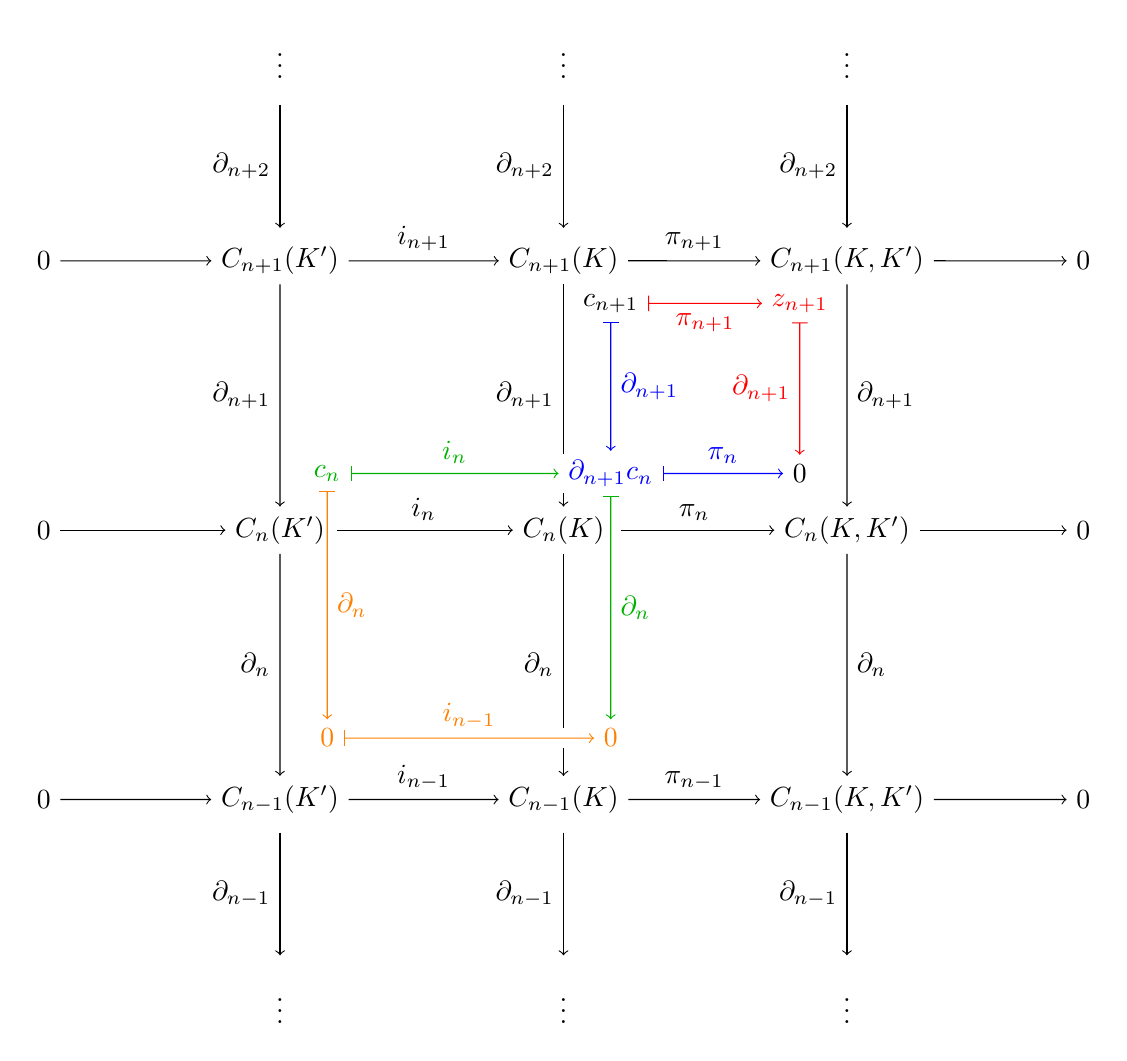
\begin{tikzpicture}[scale=1.2]
      % \draw[help lines, color=gray!30, dashed] (-1.9,-1.9) grid (6,2);
      % \draw[->] (-2,0)--(6,0) node[right]{$x$};
      % \draw[->] (0,-2)--(0,2) node[above]{$y$};

      \foreach \n/\y/\h in {n+1/2.85/t, n/0/m, n-1/-2.85/b}{
        \node (0l\h) at (-5.5, \y) {$0$};
        \node (kp\h) at (-3, \y) {$\msf C_{\n}(K')$};
        \node (k\h) at (0, \y) {$\msf C_{\n}(K)$};
        \node (kkp\h) at (3, \y) {$\msf C_{\n}(K,K')$};
        \node (0r\h) at (5.5, \y) {$0$};
        \draw[->] (0l\h) -- (kp\h);
        \draw[->] (kp\h) -- (k\h) node[midway, above] {$i_{\n}$};
        \draw[->] (k\h) -- (kkp\h) node[midway, above] {$\pi_{\n}$};
        \draw[->] (kkp\h) -- (0r\h);
      }

      \foreach \ka/\kb/\n/\side in {kpt/kpm/n+1/left, kpm/kpb/n/left, kt/km/n+1/left, km/kb/n/left, kkpt/kkpm/n+1/right, kkpm/kkpb/n/right}{
        \draw[->] (\ka) -- (\kb) node[midway, \side] {$\partial_{\n}$};
      }

      \foreach \x in {-3,0,3}{
        \draw[->] (\x, 4.5) -- (\x, 3.2) node[midway, left] {$\partial_{n+2}$};
        \draw[->] (\x, -3.2) -- (\x, -4.5) node[midway, left] {$\partial_{n-1}$};
        \node (a) at (\x, 5) {$\vdots$};
        \node (a) at (\x, -5) {$\vdots$};
      }
      \node (zn) at (2.5, 2.4) {$\color{red} z_{n+1}$};
      \node (bzn) at (2.5, .6) {$0$};
      \draw[|->, red] (zn) -- (bzn) node[midway, left] {$\partial_{n+1}$};

      \node (cn) at (.5, 2.4) {$c_{n+1}$};
      \node[blue] (bcn) at (.5, .6) {$\partial_{n+1} c_n$};
      \draw[|->, red] (cn) -- (zn) node[midway, below] {$\pi_{n+1}$};
      \draw[|->, blue] (cn) -- (bcn) node[midway, right] {$\partial_{n+1}$};
      \draw[|->, blue] (bcn) -- (bzn) node[midway, above] {$\pi_{n}$};

      \node[black!30!green] (cn-1) at (-2.5, .6) {$c_{n}$};
      \filldraw[white] (-.2,.4) rectangle (.05,.8);
      \draw[black!30!green, |->] (cn-1) -- (bcn) node[midway, above] {$i_n$};

      \filldraw[white] (-2.5, .05) rectangle (-2.4, -.05);
      \filldraw[white] (.5, .05) rectangle (.6, -.05);
      \filldraw[white] (-.05, -2.1) rectangle (.05, -2.3);

      \node[orange] (0b) at (.5, -2.2) {$0$};
      \node[orange] (0lb) at (-2.5, -2.2) {$0$};
      \draw[|->, black!30!green] (bcn) -- (0b) node[midway, right] {$\partial_n$};
      \draw[|->, orange] (cn-1) -- (0lb) node[midway, right] {$\partial_n$};
      \draw[|->, orange] (0lb) -- (0b) node[midway, above] {$i_{n-1}$};
    \end{tikzpicture}
    \caption{Diagram}
  \end{figure}
\end{solution}

\begin{definition}[Chain Complex]
  A \textbf{chain complex} $\mc{C}$ is a family $\set{C_n,
    \partial_n}$ of abelian groups $C_{n}$ and homomorphisms
  $\partial_{n}: C_{n} \to C_{n-1}$ such that $\partial_{n} \circ
  \partial_{n+1} = 0$ for all $n$. The \textbf{$n$-th homology group}
  $H_{n}(\mc{C})$ is defined by
  \[
    H_{n}(\mathcal{C}) = \ker \partial_{n} / \im \partial_{n+1}.
  \]
\end{definition}
\begin{definition}
  Given two chain complexes $\mc{C} = \set{C_n, \partial_n}$ and
  $\mc{C'}= \set{C'_n, \partial'_n}$, a \textbf{chain map} $\phi:
  \mathcal{C} \to \mathcal{C'}$ is a family of homomorphisms
  $\phi_{n}: C_{n} \to C'_{n}$ such that the $\phi_{n}$ commute with
  the boundary maps:
  \[
    \partial'_{n} \circ \phi_{n} = \phi_{n-1} \circ \partial_{n}.
  \]
\end{definition}

% \begin{problem}[The Zig-Zag Lemma]
  % Suppose
  % \[
  %   \mc C = \set{C_n, \partial^C_n} \qquad\qquad
  %   \mc D = \set{D_n, \partial^D_n} \qquad\qquad
  %   \mc E = \set{E_n, \partial^E_n}
  % \]
  % are chain complexes, and $\phi:\mathcal{C}\to\mathcal{D}$ and
  % $\psi:\mathcal{D}\to\mathcal{E}$ are chain maps such that
  % \[
  % \begin{tikzcd}
  %   0 @>>> \mathcal{C}  @>{\phi}>> \mathcal{D} @>{\psi}>> \mathcal{E} @>>> 0
  % \end{tikzcd}
  % \]
  % is a short exact sequence of chain complexes.  Then there is a long exact sequence:
  % \[
  % \begin{tikzcd}
  %   \cdots @>{\partial_{*}}>> H_{n}(\mathcal{C})   @>{\phi_{*}}>> H_{n}(\mathcal{D}) @>{\psi_{*}}>> H_{n}(\mathcal{E}) @>{\partial_{*}}>>  H_{n-1}(\mathcal{C}) @>{i_{*}}>> \cdots
  % \end{tikzcd}
  % \]
  % where $\partial_{*}$ is induced by $\partial^{D}$.
% \end{problem}

\begin{problem}[The Five Lemma]
  Consider the following commutative diagram of groups and
  homomorphisms, where the rows are exact.
  \begin{figure}[H]
    \centering
    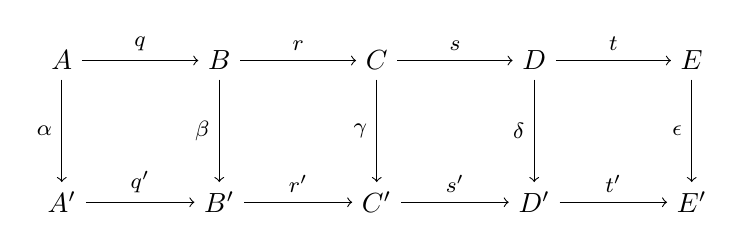
\begin{tikzpicture}
      \pgfmathsetmacro{\y}{.9};
      \foreach \letter/\x in {A/-4, B/-2, C/0, D/2, E/4}{
        \node (\letter) at (\x, \y) {$\letter$};
        \node (\letter p) at (\x, -\y) {$\letter '$};
      }

      \foreach \dom/\cod/\morphism in {A/B/q, B/C/r, C/D/s, D/E/t}{
        \draw[->] (\dom) -- (\cod) node[midway, above] {\footnotesize $\morphism$};
        \draw[->] (\dom p) -- (\cod p) node[midway, above] {\footnotesize $\morphism '$};
      }

      \foreach \letter/\letterp/\morphism in {A/Ap/\alpha, B/Bp/\beta, C/Cp/\gamma, D/Dp/\delta, E/Ep/\epsilon}{
        \draw[->] (\letter) -- (\letterp) node[midway, left] {\footnotesize $\morphism$};
      }
    \end{tikzpicture}
  \end{figure}
  If the rows are exact and $\alpha, \beta, \delta, \epsilon$ are
  isomorphisms, then $\gamma$ is also an isomorphism.
\end{problem}

\begin{solution}
  We proceed by diagram chase. We'll proceed by filling in the
  following diagram:
  \begin{figure}[H]
    \centering
    \begin{tikzpicture}[scale=1.5]
      \pgfmathsetmacro{\ybox}{1};
      \pgfmathsetmacro{\ylabel}{1.4};
      \pgfmathsetmacro{\midbox}{.825};
      \pgfmathsetmacro{\boxscale}{2.5};
      \foreach \letter/\x in {A/-4, B/-2, C/0, D/2, E/4}{
        \node[draw, scale=\boxscale] (\letter 1) at ($(\x, \ybox) + (-.25,0)$) {};
        \node[draw, scale=\boxscale] (\letter 2) at ($(\x, \ybox) + (.25,0)$) {};
        \node[draw, scale=\boxscale] (\letter 1p) at ($(\x, -\ybox) + (-.25,0)$) {};
        \node[draw, scale=\boxscale] (\letter 2p) at ($(\x, -\ybox) + (.25,0)$) {};
        \node (\letter) at (\x, \ylabel) {$\letter$};
        \node (\letter p) at (\x, -\ylabel) {$\letter '$};
      }

      \foreach \dom/\cod/\morphism in {A2/B1/q, B2/C1/r, C2/D1/s, D2/E1/t}{
        \draw[->] (\dom) -- (\cod) node[midway, above] {$\morphism$};
        \draw[->] (\dom p) -- (\cod p) node[midway, above] {$\morphism'$};
      }

      \foreach \letter/\letterp/\morphism in {A/\alpha, B/\beta, C/\gamma, D/\delta, E/\epsilon}{
        \draw[->] (\letter 1) -- (\letter 1p);
        \draw[->] (\letter 2) -- (\letter 2p);
        \draw[white, ->] ($.5*(\letter 1) + .5*(\letter 2)$) -- ($.5*(\letter 1p) + .5*(\letter 2p)$) node[midway] {$\color{black} \morphism$};
        % \draw[->] (\letter 1) -- (\letter 1p) node[midway, left] {$\morphism$};
        % \draw[->] (\letter 2) -- (\letter 2p) node[midway, right] {$\morphism$};
      }
    \end{tikzpicture}
  \end{figure}
  First, we show $\gamma$ is injective. To that end, we want to show
  $\ker \gamma = \set{0}$.

  Let $c \in C$, and suppose $c \in \ker \gamma$. Then $\gamma(c) =
  0$, hence $\gamma(c) \in \ker r'$. Thus by exactness, there exists
  $a' \in A'$, $b' \in B'$ such that $q'(a') = b'$, and $r'(b') =
  \gamma(c) = 0$:
  \begin{figure}[H]
    \centering
    \begin{tikzpicture}[scale=1.5]
      \pgfmathsetmacro{\ybox}{1};
      \pgfmathsetmacro{\ylabel}{1.4};
      \pgfmathsetmacro{\midbox}{.825};
      \pgfmathsetmacro{\boxscale}{2.5};
      \foreach \letter/\x in {A/-4, B/-2, C/0, D/2, E/4}{
        \node[draw, scale=\boxscale] (\letter 1) at ($(\x, \ybox) + (-.25,0)$) {};
        \node[draw, scale=\boxscale] (\letter 2) at ($(\x, \ybox) + (.25,0)$) {};
        \node[draw, scale=\boxscale] (\letter 1p) at ($(\x, -\ybox) + (-.25,0)$) {};
        \node[draw, scale=\boxscale] (\letter 2p) at ($(\x, -\ybox) + (.25,0)$) {};
        \node (\letter) at (\x, \ylabel) {$\letter$};
        \node (\letter p) at (\x, -\ylabel) {$\letter '$};
      }

      \foreach \dom/\cod/\morphism in {A2/B1/q, B2/C1/r, C2/D1/s, D2/E1/t}{
        \draw[->] (\dom) -- (\cod) node[midway, above] {$\morphism$};
        \draw[->] (\dom p) -- (\cod p) node[midway, above] {$\morphism'$};
      }

      \foreach \letter/\letterp/\morphism in {A/\alpha, B/\beta, C/\gamma, D/\delta, E/\epsilon}{
        \draw[->] (\letter 1) -- (\letter 1p);
        \draw[->] (\letter 2) -- (\letter 2p);
        \draw[white, ->] ($.5*(\letter 1) + .5*(\letter 2)$) -- ($.5*(\letter 1p) + .5*(\letter 2p)$) node[midway] {$\color{black} \morphism$};
        % \draw[->] (\letter 1) -- (\letter 1p) node[midway, left] {$\morphism$};
        % \draw[->] (\letter 2) -- (\letter 2p) node[midway, right] {$\morphism$};
      }
      \node[red] at (C1) {\footnotesize $c$};
      \node[red] at (A1p) {\footnotesize $a'$};
      \node[red] at (B1p) {\footnotesize $b'$};
      \node[red] at (C1p) {\footnotesize $0$};
    \end{tikzpicture}
  \end{figure}
  Now, since $\alpha, \beta$ are surjective, there exists $a \in A$,
  $b \in B$ such that $\alpha(a) = a'$, $\beta(b) = b'$:
  \begin{figure}[H]
    \centering
    \begin{tikzpicture}[scale=1.5]
      \pgfmathsetmacro{\ybox}{1};
      \pgfmathsetmacro{\ylabel}{1.4};
      \pgfmathsetmacro{\midbox}{.825};
      \pgfmathsetmacro{\boxscale}{2.5};
      \foreach \letter/\x in {A/-4, B/-2, C/0, D/2, E/4}{
        \node[draw, scale=\boxscale] (\letter 1) at ($(\x, \ybox) + (-.25,0)$) {};
        \node[draw, scale=\boxscale] (\letter 2) at ($(\x, \ybox) + (.25,0)$) {};
        \node[draw, scale=\boxscale] (\letter 1p) at ($(\x, -\ybox) + (-.25,0)$) {};
        \node[draw, scale=\boxscale] (\letter 2p) at ($(\x, -\ybox) + (.25,0)$) {};
        \node (\letter) at (\x, \ylabel) {$\letter$};
        \node (\letter p) at (\x, -\ylabel) {$\letter '$};
      }

      \foreach \dom/\cod/\morphism in {A2/B1/q, B2/C1/r, C2/D1/s, D2/E1/t}{
        \draw[->] (\dom) -- (\cod) node[midway, above] {$\morphism$};
        \draw[->] (\dom p) -- (\cod p) node[midway, above] {$\morphism'$};
      }

      \foreach \letter/\letterp/\morphism in {A/\alpha, B/\beta, C/\gamma, D/\delta, E/\epsilon}{
        \draw[->] (\letter 1) -- (\letter 1p);
        \draw[->] (\letter 2) -- (\letter 2p);
        \draw[white, ->] ($.5*(\letter 1) + .5*(\letter 2)$) -- ($.5*(\letter 1p) + .5*(\letter 2p)$) node[midway] {$\color{black} \morphism$};
        % \draw[->] (\letter 1) -- (\letter 1p) node[midway, left] {$\morphism$};
        % \draw[->] (\letter 2) -- (\letter 2p) node[midway, right] {$\morphism$};
      }

      \node[red] at (A1) {\footnotesize $a$};
      \draw[white, ->] (A1) -- (A1p);
      \draw[red, thick, ->>] (A1) -- (A1p);
      \node[red] at (B1) {\footnotesize $b$};
      \draw[white, ->] (B1) -- (B1p);
      \draw[red, thick, ->>] (B1) -- (B1p);

      \node at (C1) {\footnotesize $c$};
      \node at (A1p) {\footnotesize $a'$};
      \node at (B1p) {\footnotesize $b'$};
      \node at (C1p) {\footnotesize $0$};
    \end{tikzpicture}
    \caption{Surjectivity, indicated by the double arrowhead.}
  \end{figure}
  Now, note that $s'(\gamma(c)) = s'(0) = 0$. Since $\delta$ is
  an isomorphism (and thus injective), it follows that
  $\delta^{-1}(\gamma(c)) = \delta^{-1}(0) = 0$. Finally, by
  commutativity of the square, we have $s(c) = 0$, so we can place
  them in corresponding boxes:
  \begin{figure}[H]
    \centering
    \begin{tikzpicture}[scale=1.5]
      \pgfmathsetmacro{\ybox}{1};
      \pgfmathsetmacro{\ylabel}{1.4};
      \pgfmathsetmacro{\midbox}{.825};
      \pgfmathsetmacro{\boxscale}{2.5};
      \foreach \letter/\x in {A/-4, B/-2, C/0, D/2, E/4}{
        \node[draw, scale=\boxscale] (\letter 1) at ($(\x, \ybox) + (-.25,0)$) {};
        \node[draw, scale=\boxscale] (\letter 2) at ($(\x, \ybox) + (.25,0)$) {};
        \node[draw, scale=\boxscale] (\letter 1p) at ($(\x, -\ybox) + (-.25,0)$) {};
        \node[draw, scale=\boxscale] (\letter 2p) at ($(\x, -\ybox) + (.25,0)$) {};
        \node (\letter) at (\x, \ylabel) {$\letter$};
        \node (\letter p) at (\x, -\ylabel) {$\letter '$};
      }

      \foreach \dom/\cod/\morphism in {A2/B1/q, B2/C1/r, C2/D1/s, D2/E1/t}{
        \draw[->] (\dom) -- (\cod) node[midway, above] {$\morphism$};
        \draw[->] (\dom p) -- (\cod p) node[midway, above] {$\morphism'$};
      }

      \foreach \letter/\letterp/\morphism in {A/\alpha, B/\beta, C/\gamma, D/\delta, E/\epsilon}{
        \draw[->] (\letter 1) -- (\letter 1p);
        \draw[->] (\letter 2) -- (\letter 2p);
        \draw[white, ->] ($.5*(\letter 1) + .5*(\letter 2)$) -- ($.5*(\letter 1p) + .5*(\letter 2p)$) node[midway] {$\color{black} \morphism$};
        % \draw[->] (\letter 1) -- (\letter 1p) node[midway, left] {$\morphism$};
        % \draw[->] (\letter 2) -- (\letter 2p) node[midway, right] {$\morphism$};
      }

      \draw[white, ->] (A1) -- (A1p);
      \draw[thick, ->>] (A1) -- (A1p);
      \node at (B1) {\footnotesize $b$};
      \draw[white, ->] (B1) -- (B1p);
      \draw[thick, ->>] (B1) -- (B1p);

      \node at (C1) {\footnotesize $c$};
      \node at (A1p) {\footnotesize $a'$};
      \node at (B1p) {\footnotesize $b'$};
      \node at (C1p) {\footnotesize $0$};

      \node at (A1) {\footnotesize $a$};

      \node[red] at (D1p) {\footnotesize $0$};
      \node[red] at (D1) {\footnotesize $0$};
      \draw[white, ->] (D1) -- (D1p);
      \draw[white, thick] (D1) -- (D1p);
      \draw[red, thick, arrows={Hooks[right, length=1mm]->}] (D1) -- (D1p);
      \draw[red, thick, ->] (1.375,0) arc (0:330:.375);
    \end{tikzpicture}
    \caption{Injectivity, indicated by the hooked arrow, and
      commutativity.}
  \end{figure}
  Now, $c \in \ker s$ implies $c \in \im r$, thus there exists $\ol b
  \in B$ such that $r(\ol b) = c$. Let $\ol{b}' = \beta(b)$. Then by
  commutativity,
  \[
    r'\pn{\ol{b}'} = (r' \circ \beta)(\ol{b}) = (\gamma \circ
    r)(\ol{b}) = 0
  \]
  and thus $\ol{b}' \in \ker r'$. By exactness, there exists $\ol{a}'
  \in A'$ such that $q'\pn{\ol{a}'} = \ol{b}'$:
  \begin{figure}[H]
    \centering
    \begin{tikzpicture}[scale=1.5]
      \pgfmathsetmacro{\ybox}{1};
      \pgfmathsetmacro{\ylabel}{1.4};
      \pgfmathsetmacro{\midbox}{.825};
      \pgfmathsetmacro{\boxscale}{2.5};
      \foreach \letter/\x in {A/-4, B/-2, C/0, D/2, E/4}{
        \node[draw, scale=\boxscale] (\letter 1) at ($(\x, \ybox) + (-.25,0)$) {};
        \node[draw, scale=\boxscale] (\letter 2) at ($(\x, \ybox) + (.25,0)$) {};
        \node[draw, scale=\boxscale] (\letter 1p) at ($(\x, -\ybox) + (-.25,0)$) {};
        \node[draw, scale=\boxscale] (\letter 2p) at ($(\x, -\ybox) + (.25,0)$) {};
        \node (\letter) at (\x, \ylabel) {$\letter$};
        \node (\letter p) at (\x, -\ylabel) {$\letter '$};
      }

      \foreach \dom/\cod/\morphism in {A2/B1/q, B2/C1/r, C2/D1/s, D2/E1/t}{
        \draw[->] (\dom) -- (\cod) node[midway, above] {$\morphism$};
        \draw[->] (\dom p) -- (\cod p) node[midway, above] {$\morphism'$};
      }

      \foreach \letter/\letterp/\morphism in {A/\alpha, B/\beta, C/\gamma, D/\delta, E/\epsilon}{
        \draw[->] (\letter 1) -- (\letter 1p);
        \draw[->] (\letter 2) -- (\letter 2p);
        \draw[white, ->] ($.5*(\letter 1) + .5*(\letter 2)$) -- ($.5*(\letter 1p) + .5*(\letter 2p)$) node[midway] {$\color{black} \morphism$};
      }

      \node at (A1) {\footnotesize $a$};
      \draw[white, ->] (A1) -- (A1p);
      \draw[thick, ->>] (A1) -- (A1p);
      \node at (B1) {\footnotesize $b$};
      \draw[white, ->] (B1) -- (B1p);
      \draw[thick, ->>] (B1) -- (B1p);

      \node at (C1) {\footnotesize $c$};
      \node at (A1p) {\footnotesize $a'$};
      \node at (B1p) {\footnotesize $b'$};
      \node at (C1p) {\footnotesize $0$};

      \node at (D1p) {\footnotesize $0$};
      \node at (D1) {\footnotesize $0$};
      \draw[white, ->] (D1) -- (D1p);
      \draw[white, thick] (D1) -- (D1p);
      \draw[thick, arrows={Hooks[right, length=1mm]->}] (D1) -- (D1p);
      \draw[thick, ->] (1.375,0) arc (0:330:.375);

      \draw[white, ->] (B2) -- (B2p);
      \draw[red, thick, ->] (B2) -- (B2p);
      \node[red] at (B2) {\footnotesize $\color{red}\ol b$};
      \node[red] at (B2p) {\footnotesize $\color{red}\ol{b}'$};
      \node[red] at (A2p) {\footnotesize $\color{red}\ol{a}'$};
      \draw[red, thick, ->] (-.625,0) arc (0:330:.375);
    \end{tikzpicture}
    \caption{}
  \end{figure}
  Using surjectivity of $\alpha$, there exists $\ol a \in A$ such that
  $\alpha(\ol a) = \ol{a}'$. Then
  \begin{align*}
    r(\ol b)
    &= r(q(\ol a)) \\
    &= (r\circ q)(\ol a) \\
    &= 0
  \end{align*}
  where the last portion follows by exactness. Thus, $\gamma$ is
  injective.
  \begin{remark}
    My argument was actually somewhat redundant here. I just didn't
    adjust it because that would have required lots of re-\TeX ing of
    diagrams.
  \end{remark}
  We'll attempt a less-redundant argument for surjectivity. We'll fill
  in the following diagram:
  \begin{figure}[H]
    \centering
    \begin{tikzpicture}[scale=1.5]
      \pgfmathsetmacro{\ybox}{1};
      \pgfmathsetmacro{\ylabel}{2};
      \pgfmathsetmacro{\midbox}{.825};
      \pgfmathsetmacro{\boxscale}{2.5};
      \foreach \letter/\x in {A/-4, B/-2, C/0, D/2, E/4}{
        \node[draw, scale=\boxscale] (\letter 1) at ($(\x, \ybox) + (-.25,0)$) {};
        \node[draw, scale=\boxscale] (\letter 2) at ($(\x, \ybox) + (.25,0)$) {};
        \node[draw, scale=\boxscale] (\letter 1p) at ($(\x, -\ybox) + (-.25,0)$) {};
        \node[draw, scale=\boxscale] (\letter 2p) at ($(\x, -\ybox) + (.25,0)$) {};
        \node (\letter) at (\x, \ylabel) {$\letter$};
        \node (\letter p) at (\x, -\ylabel) {$\letter '$};
      }
    \end{tikzpicture}
  \end{figure}
  Let $c' \in C$. Then $d' = s'(c') \in D'$, and $t'(d') = t'(s'(c'))
  = 0$:
  \begin{figure}[H]
    \centering
    \begin{tikzpicture}[scale=1.5]
      \pgfmathsetmacro{\ybox}{1};
      \pgfmathsetmacro{\ylabel}{2};
      \pgfmathsetmacro{\midbox}{.825};
      \pgfmathsetmacro{\boxscale}{2.5};
      \foreach \letter/\x in {A/-4, B/-2, C/0, D/2, E/4}{
        \node[draw, scale=\boxscale] (\letter 1) at ($(\x, \ybox) + (-.25,0)$) {};
        \node[draw, scale=\boxscale] (\letter 2) at ($(\x, \ybox) + (.25,0)$) {};
        \node[draw, scale=\boxscale] (\letter 1p) at ($(\x, -\ybox) + (-.25,0)$) {};
        \node[draw, scale=\boxscale] (\letter 2p) at ($(\x, -\ybox) + (.25,0)$) {};
        \node (\letter) at (\x, \ylabel) {$\letter$};
        \node (\letter p) at (\x, -\ylabel) {$\letter '$};
      }

      \node[red] at (C2p) {$c'$};
      \node[red] at (D1p) {$d'$};
      \draw[red, thick, ->] (C2p) -- (D1p) node[midway, below] {$s'$};

      \node[red] at (E1p) {$0$};

    \end{tikzpicture}
  \end{figure}
  % By surjectivity of $\delta$, $\exists d \in D$ such that $$
\end{solution}

\section{Useful Exact Sequences}
\begin{problem}[18.32 (Long Exact Sequence of a Pair)]
  If $K'$ is a subcomplex of a simplicial complex $K$, then there is a
  long exact sequence:
  \begin{center}
    \begin{tikzpicture}
      \node (lcdots) at (-5,0) {$\cdots$};
      \node (hnkp) at (-3,0) {$H_n(K')$};
      \node (hnk) at (0,0) {$H_n(K)$};
      \node (hnkkp) at (3,0) {$H_n(K,K')$};
      \node (hnmo) at (6,0) {$H_{n-1}(K')$};
      \node (rcdots) at (8,0) {$\cdots$};
      \draw[->] (lcdots) -- (hnkp) node[midway, above] {$\partial_*$};
      \draw[->] (hnkp) -- (hnk) node[midway, above] {$i_*$};
      \draw[->] (hnk) -- (hnkkp) node[midway, above] {$\pi_*$};
      \draw[->] (hnkkp) -- (hnmo) node[midway, above] {$\partial_*$};
      \draw[->] (hnmo) -- (rcdots) node[midway, above] {$i_*$};
    \end{tikzpicture}
  \end{center}
  where the maps are induced by the inclusion maps $i : K' \to K$ and
  $\pi : (K,\varnothing) \to (K,K')$ and the boundary map $\partial :
  C_n(X) \to C_{n-1}(x)$.
\end{problem}
\begin{solution}
  Follows as a corollary of the Zig-Zag Lemma.
\end{solution}
\section{The Degree of a Map}
% \begin{problem}[Review]
%   Show that $H_n(\sS^n) \cong \ZZ$
% \end{problem}
% \begin{solution}

% \end{solution}

\begin{definition}
  Let $f : \sS^n \to \sS^n$ be a continuous map. Then $f_* :
  H_n(\sS^n) \to H_n(\sS^n)$ is a homomorphism from $\ZZ$ to itself.
  Hence it represent multiplication by some integer, called the
  \emph{degree} of $f$ and denoted $\deg f$.
\end{definition}
\begin{problem}[18.38]
  If $f : \sS^n \to \sS^n$ is continuous, then $\deg f$ is
  well-defined. That is, it does not depend on the way in which we
  identify $H_n(\sS^n)$ with $\ZZ$.
\end{problem}
\begin{solution}
  ?
  % Let $f_*^{(1)}, f_^{(2)}$ be
\end{solution}
\begin{problem}[18.39]
  Let $f,g : \sS^n \to \sS^n$ be continuous maps.
  \begin{enumerate}
    \item If $f$ and $g$ are homotopic, they have the same degree.
    \item $\deg (f \circ g) = (\deg f) \cdot (\deg g)$.
  \end{enumerate}
\end{problem}
\begin{solution}
  \begin{enumerate}
    \item Since $f,g$ are homotopic, there exists a continuous map $F
      : \sS^n \times [0,1] \to \sS^n$ such that $F(\bm x, 0) = f(\bm
      x)$, and $F(\bm x, 1) = g(\bm x)$.
    \item
  \end{enumerate}
\end{solution}

\section{Lefschetz}
\begin{definition}[Free Abelian Group]
  A group
  \[
    G \cong \osum_{i=1}^n \ZZ
  \]
  is called the \emph{free abelian group of rank $n$}.
\end{definition}
\begin{definition}[Torsion Group]
  Let $G$ be a group. Denote the \emph{torsion subgroup}, $G_{\rm
    tor}$, by
  \[
    G_{\rm tor} = \set{g \in G \MID \exists n \in \NN \st g^n =
      \epsilon},
  \]
  that is, the subgroup of all elements with finite order.
\end{definition}
\begin{problem}[FK]
  Prove that $G_{\rm tor}$ is indeed a subgroup of $G$.
\end{problem}
\begin{solution}
  Let $g_1, g_2 \in G_{\rm tor}$. WTS $g_1 g_2^{-1} \in G_{\rm tor}$.
  % Then $\exists n_1, n_2 \in \NN \st$
  % \[
  %   g_1^{n_1} = \epsilon, \qquad\qquad\qquad g_2^{n_2} = \epsilon.
  % \]
  % WTS $g_1g_2$ has finite order. Let $k = \lcm(n_1, n_2)$. Then
  % $\exists m_1, m_2 \in \NN \st n_1 =m_1 k$, and $n_2 = m_2 k$. Now,
  % \begin{align*}

  % \end{align*}
\end{solution}
\begin{definition}
  Let $G$ be a finitely generated abelian group, which we can express
  as
  \[
    G = G_{\rm free} \oplus G_{\rm tor},
  \]
  the direct sum of a free and a torsion group.
\end{definition}

%%% Local Variables:
%%% TeX-master: "../main"
%%% TeX-engine: default-shell-escape
%%% TeX-command-extra-option: -pdf
%%% End:
\chapter{Some Homological Algebra}
The big idea: algebraic topology assigns discrete algebraic invariants to
topological spaces and continuous maps. Book for this section: James May's
\emph{A Concise Course in Algebraic Topology}

\section{Chain complexes}
\begin{definition}[Chain/Cochain Complexes]
  Let $R$ be a commutative ring. A \emph{chain complex} over $R$ is a sequence
  of maps of $R$-modules
  \[
    \cdots \rightarrow X_{i+1} \xrightarrow{d_{i+1}} X_i \xrightarrow{d_i}
    X_{i-1} \rightarrow \cdots
  \]
  such that $d_i \circ d_{i+1} = 0$ for all $i$. We generally abbreviate $d =
  d_i$. A \emph{cochain complex} over $R$ is an analogous sequence
  \[
    \cdots \rightarrow Y^{i-1} \xrightarrow{d^{i-1}} Y^i \xrightarrow{d^i}
    Y^{i-1} \rightarrow \cdots
  \]
  with $d^i \circ d^{i-1}$.

  We usually require chain complexes to satisfy $X_i = 0$ for $i < 0$, and
  cochain complexes to satisfy $Y^i = 0$ for $i < 0$. Without this distinction,
  the definitions are equivalent.
\end{definition}
\begin{definition}[Some definitions]
  Elements of $\ker d_i$ are called cycles. Elements of $\im d_{i+1}$ are called
  boundaries. Write $B_i(X) \subset Z_i(X) \subset X_i$ for the submodules of
  boundaries and dycles, and define the $i$\textsuperscript{th} homology group
  $H_i(X)$ by
  \[
    H_i(X) = Z_i(X) / B_i(X).
  \]
  We write $H_*(X)$ for the sequence of $R$-modules $H_i(X)$. We understand
\end{definition}

%%% Local Variables:
%%% TeX-master: "../main"
%%% End:
\chapter{Rotman}
The big idea: algebraic topology assigns discrete algebraic invariants to
topological spaces and continuous maps. Book for this section: Joseph Rotman's
\emph{A First Course in Algebraic Topology}

\section{A sketch of the Brouwer Fixed Point Theorem}
\begin{problem}[R 0.1]
  Every continuous function $f : D^1 \to D^1$ has a fixed point.
\end{problem}
\begin{solution}
  We'll prove this without the techniques of analysis, so as to make the
  connection to the general argument slightly more obvious. Let $f(-1) = a$ and
  $f(1) = b$.
  \begin{enumerate}[label=(\arabic*)]
    \item Suppose $a = -1$ or $b = 1$, then we're done.
    \item Else, $a > -1$ and $b < 1$. Consider the graph of $f$:
      \[
        G = \set{\pn{x, f(x)} \MID x \in D^1}
      \]
      since $f$ is continuous and $D^1$ is connected, $G$ is connected as well.
      Let
      \[
        A = \set{\pn{x, f(x)} \MID f(x) > x} \qquad \text{and} \qquad B =
        \set{\pn{x, f(x)} \MID f(x) < x}.
      \]
      \begin{figure}[H]
        \centering
        \begin{tikzpicture}[scale=2]
          \path
          coordinate (1) at (-1,-1)
          coordinate (2) at (-1,1)
          coordinate (3) at (1,1)
          coordinate (4) at (1,-1)
          coordinate (a) at (-1,-.3)
          coordinate (b) at (1, .4);

          \foreach \v in {1,2,3,4}{
            \draw[fill=black] (\v) circle (0.5pt);
          }

          \node[below left] (11) at (1) {$(-1,-1)$};
          \node[above left] (21) at (2) {$(-1,1)$};
          \node[above right] (31) at (3) {$(1,1)$};
          \node[below right] (41) at (4) {$(1,-1)$};

          \draw (1) -- (2) -- (3) -- (4) -- (1);
          \draw (1) -- (3);

          \draw[fill=blue] (a) circle (0.75pt);
          \draw[fill=red] (b) circle (0.75pt);
          \node[left] (ap) at (a) {$\color{blue}a$};
          \node[right] (bp) at (b) {$\color{red}b$};

          % \draw[domain=-1:1,smooth,variable=\x,blue] plot ({\x},{(-24 - 101*\x + 27*\x^2 + 122*\x^3)/60});
          \draw[domain=-1:-0.0405889,smooth,variable=\x,blue] plot ({\x},{\x*(\x*(1.4*\x + 0.133333) - 1.05) - 0.0833333});
          \draw[domain=-0.0405889:1,smooth,variable=\x,red] plot ({\x},{\x*(\x*(1.4*\x + 0.133333) - 1.05) - 0.0833333});

        \end{tikzpicture}
        \caption{$G$}
        \label{fig:brouwer-1}
      \end{figure}
      And let $\Delta = \set{\pn{x,x} \MID x \in [0,1]}$. Note $a \in A$, and $b
      \in B$, so $A \neq \varnothing \neq B$.

      Suppose $G \cap \Delta = \varnothing$. Then $G = A \sqcup B$. Note $A,B$
      are open in $G$, hence $G$ is not connected, a contradiction.
  \end{enumerate}
\end{solution}

\begin{definition}[retract]
  A subspace $X$ of a topological space $Y$ is a \emph{retract} of $Y$ if there
  is a continuous map $r : Y \to Y$ with $r(x) = x$ for all $x \in X$. Such a
  map is called a \emph{retraction}.
\end{definition}

% \begin{problem}[R 0.2]
%   If $n \geq 0$, then $S^n$ is not a retract of $D^{n+1}$
% \end{problem}
% \begin{solution}

% \end{solution}

\begin{problem}

\end{problem}

%%% Local Variables:
%%% TeX-master: "../main"
%%% End:

\chapter{Appendix}
\section{List of Definitions}
\listofdefinitions

\end{document}
%%% Local Variables:
%%% TeX-master: t
%%% TeX-engine: default-shell-escape
%%% TeX-command-extra-option: -pdf
%%% End: